% Template for bachelor's/master's thesis for students at Karlsruhe Institute of Technology.
% Best for students majored in Computer Science or Mathematics.

% English version by Wei Zhou (ftfish@gmail.com)
% Based on the German version of Timo Bingmann


% This is just a template. Since there's no strict rule on how a bachelor's thesis must look like, every part of this template can be adapted.

\documentclass[12pt,a4paper,twoside]{scrartcl}

% Loading babel to enable automatic hypentation and multiple languages in the document.
% The last language in the option list will be used as default.
\usepackage[ngerman,english]{babel}
% Using T1 font encoding and the Latin Modern font
\usepackage[T1]{fontenc}
\usepackage{lmodern}
\usepackage{lscape}
\usepackage{afterpage}

% Using utf8 as file encoding.
\usepackage[utf8]{inputenc}
\usepackage[capbesideposition=outside,capbesidesep=quad]{floatrow}


% Page size. Using almost the whole A4 paper.
\usepackage[tmargin=22mm,bmargin=22mm,lmargin=20mm,rmargin=20mm]{geometry}


% Some standard packages for writing papers
\usepackage{latexsym,amsmath,amssymb,mathtools,textcomp}

% Paragraphs are not indented but there will be some space between paragraphs
\usepackage{parskip}
% For defining theorem-style environments like Lemma/Proof/Definition
\usepackage{amsthm}
% Fixing spacing problems before theorems due to \usepackage{parskip}
\begingroup
    \makeatletter
    \@for\theoremstyle:=definition,remark,plain\do{%
        \expandafter\g@addto@macro\csname th@\theoremstyle\endcsname{%
            \addtolength\thm@preskip\parskip
            }%
        }
\endgroup

% Some theorem-style environments
\newtheorem{theorem}{Theorem}[section]
\newtheorem{definition}[theorem]{Definition}
\newtheorem{lemma}[theorem]{Lemma}

% Setting equation numbers to <chapter>.<section>.<index>
\numberwithin{equation}{section}

% For inserting graphics into the document
\usepackage{graphicx}
\graphicspath{{images/}}

% For tables
\usepackage{array,multirow}

% Control layout of itemize, enumerate, description
\usepackage{enumitem}

\setlist[enumerate]{topsep=0pt}
\setlist[itemize]{topsep=0pt}
\setlist[description]{font=\normalfont,topsep=0pt}

\setlist[enumerate,1]{label=(\roman*)}

% TikZ for graphics in LaTeX
\usepackage{tikz}
\usetikzlibrary{calc}

% Have the current section and subsection in the header.
\usepackage{fancyhdr}
\usepackage{ltxtable} 
\fancypagestyle{plain}{
  \setlength\footskip{32pt}
  \fancyhead{}
  \fancyfoot{}
  \fancyfoot[LE,RO]{\normalsize\thepage}
  \renewcommand{\headrulewidth}{0pt}
  \renewcommand{\footrulewidth}{0pt}
}

\fancypagestyle{normal}{
  \setlength{\headheight}{20pt}
  \setlength\footskip{32pt}
  \fancyhead{}
  \fancyhead[LE]{\normalsize\textsc{\nouppercase{\leftmark}}}
  \fancyhead[RO]{\normalsize\textsc{\nouppercase{\rightmark}}}
  \fancyfoot{}
  \fancyfoot[LE,RO]{\normalsize\thepage}
  \renewcommand{\headrulewidth}{0.4pt}
  \renewcommand{\footrulewidth}{0pt}
}

% Hyperref for hyperlinks und cross refs
\usepackage{color}
\usepackage{lscape}
\usepackage[pagebackref]{hyperref}
\usepackage[all]{hypcap}
\usepackage{pbox}
\DeclareOldFontCommand{\bf}{\normalfont\bfseries}{\mathbf}
\hypersetup{
  pdftitle={Solving the Graph Coloring Problem with
Cooperative Local Search}, %TODO
  pdfauthor={Guangping Li}, %TODO
  pdfsubject={Tabucol, \emph{\textbf{graph coloring problem}},parallel cooperative tabu search}, %TODO
  colorlinks=true,
  pdfborder={0 0 0},
  bookmarksopen=true,
  bookmarksopenlevel=1,
  bookmarksnumbered=true,
  linkcolor=black,
  %linkcolor=black,
  citecolor=black,
  urlcolor=black,
  filecolor=black,
  pdfpagemode=UseNone,
  unicode=true,
}

% Add the word "page" for pagebackref's in the bibliography.
\renewcommand*{\backreflastsep}{, }
\renewcommand*{\backreftwosep}{, }
\renewcommand*{\backref}[1]{}
\renewcommand*{\backrefalt}[4]{%
  \ifcase #1 %
No citations.% use \relax if you do not want the "No citations" message %TODO
  \or
(Page #2).%
  \else
(Pages #2).%
  \fi%
}


% For importing graphics from subdirectories.
\usepackage{import}

% Referencing figures, etc.
\newcommand{\reflst}[1]{\hyperref[#1]{Listing~\ref*{#1}}}
\newcommand{\refthm}[1]{\hyperref[#1]{Theorem~\ref*{#1}}}
\newcommand{\refdef}[1]{\hyperref[#1]{Definition~\ref*{#1}}}




% Package for inserting pseudo codes in the document.
\usepackage[ruled,vlined,linesnumbered,norelsize]{algorithm2e}
\DontPrintSemicolon
\def\NlSty#1{\textnormal{\fontsize{8}{10}\selectfont{}#1}}
\SetKwSty{texttt}
\SetCommentSty{emph}
\def\listalgorithmcfname{List of Algorithms}
\def\algorithmautorefname{Algorithm}
\let\chapter=\section % resolve a problem with algorithm2e

\begin{document}

%%%%%%%%%%%%%%%%%%%%%%%%%%%%%%%%%%%%%%%%%%%%%%%%%%%%%%%%%%%%%%%%%%%%%%
\pagestyle{empty} % no page number
\pagenumbering{alph}

% title page
\begin{titlepage}

  \begin{center}\large

    {\flushleft
\includegraphics[height=17mm]{kit_logo_en.pdf} \hfill}
%    \includegraphics[height=20mm]{grouplogo-algo-blue.pdf}\quad\null

    \vfill

    \vspace*{2cm}

    {\bf\huge Solving the Graph Coloring Problem  \\ with Cooperative Local Search \par} %TODO
    % Be sure to fill in the field pdftitle={} above
    % mit \par am Ende stimmt der Zeilenabstand
  

    \vfill
Bachelor Thesis of \\

    \vspace*{15mm}
    {\bf Guangping Li} %TODO

    \vspace*{15mm}

    At the Department of Informatics\\
Institute of Theoretical informatics, Algorithmics II %TODO

    \vspace*{45mm}

    \begin{tabular}{rl}
      Advisors: & Dr. Tom{\' a}{\v s} Balyo \\ %TODO
      & Prof. Dr. Peter Sanders  \\
    \end{tabular}
    
    \vspace*{10mm}

	% Deutsch
%    Institut für Theoretische Informatik, Algorithmik \\
%    Fakultät für Informatik \\
%    Karlsruher Institut für Technologie

    % English:
%     Institute of Theoretical Informatics, Algorithmics \\

    \vspace*{12mm}
  \end{center}
\afterpage{\null\newpage}
\end{titlepage}
\afterpage{\null\newpage}
%%%%%%%%%%%%%%%%%%%%%%%%%%%%%%%%%%%%%%%%%%%%%%%%%%%%%%%%%%%%%%%%%%%%%%
\vspace*{0pt}\vfill

\selectlanguage{ngerman}
\hrule\medskip

Hiermit versichere ich, dass ich diese Arbeit selbständig verfasst und keine anderen, als die angegebenen Quellen und Hilfsmittel benutzt, die wörtlich oder inhaltlich übernommenen Stellen als solche kenntlich gemacht und die Satzung des Karlsruher Instituts für Technologie zur Sicherung guter wissenschaftlicher Praxis in der jeweils gültigen Fassung beachtet habe.

\bigskip

\noindent
Karlsruhe, 15th December 2016 %TODO

% Hand-written signature!! %TODO

\vspace*{5cm}

\clearpage

%%%%%%%%%%%%%%%%%%%%%%%%%%%%%%%%%%%%%%%%%%%%%%%%%%%%%%%%%%%%%%%%%%%%%%

\vspace*{0pt}\vfill
\selectlanguage{english}
\begin{abstract}
\centerline{\bf Abstract}
{\noindent Tabucol is a local search algorithm to determine whether the vertices of an undirected graph can be colored with $k$ colors, such that no two vertices connected by an edge have the same color. This thesis presents an algorithm that
solves the graph coloring problem with parallel Tabucol searches. A hypothesis was experimentally evaluated that sharing information among the agents will improve the performance of the parallel search. In this paper, we introduce a new matrix data structure, which counts the repeated times of one change. This statistic matrix can help recognizing long-term cycling in the local search. The sharing of this matrix among the agents can bring further improvement to our algorithm.}

\end{abstract}
\vfill
\afterpage{\null\newpage}
\selectlanguage{ngerman}
\begin{abstract}
\centerline{\bf Zusammenfassung}
{\noindent Diese Arbeit präsentiert einen Algorithmus, der eine gültige  $k$-Knotenfärbung für ungerichtete Graph mit minimal $k$ sucht. Der Algorithmus macht sich dabei einen lokalen Algorithmus Tabucol zu Nutzung. Die Leistung mit verschiedenen Strategien wurde anhand von mehreren Experimenten evaluiert und miteinander verglichen. Dabei zeigt der parallel laufende
Algorithmus mit geeignetem Informationsaustausch unter den Agenten eine Verbesserung in Bezug auf Leistung aus. Wir stellen in diesem Papier eine neue Matrix Data Struktur vor, die die Wiederholung einer lokalen Änderung zählt. Diese Statistik Matrix kann helfen, lange Zyklen in der lokalen Suche zu erkennen. Das Teilen dieser Matrix unter den Agenten kann eine weitere Verbesserung unseres Algorithmus bringen.}
\end{abstract}


\vfill\vfill\vfill
\clearpage

%%%%%%%%%%%%%%%%%%%%%%%%%%%%%%%%%%%%%%%%%%%%%%%%%%%%%%%%%%%%%%%%%%%%%%

\selectlanguage{english}
\pagestyle{plain}
\pagenumbering{roman}
  
% markiere sections im Seitenkopf links und subsections rechts
\renewcommand\sectionmark[1]{\markboth{\thesection\quad\MakeUppercase{#1}}{\thesection\quad\MakeUppercase{#1}}}
\renewcommand\subsectionmark[1]{\markright{\thesubsection\quad\MakeUppercase{#1}}}


\tableofcontents
\afterpage{\null\newpage}
\clearpage

%%%%%%%%%%%%%%%%%%%%%%%%%%%%%%%%%%%%%%%%%%%%%%%%%%%%%%%%%%%%%%%%%%%%%%
%%%%%%%%%%%%%%%%%%%%%%%%%%%%%%%%%%%%%%%%%%%%%%%%%%%%%%%%%%%%%%%%%%%%%%
\pagestyle{normal}
\pagenumbering{arabic}

\section{Introduction}
\subsection{Problem/Motivation}The \emph{\textbf{graph coloring problem}}
(\emph{\textbf{GCP}}) \cite{kubale2004graph} is an NP-complete problem \cite{gary1979computers}. The problem is to assign colors to certain elements of a graph subject to certain constraints.

\emph{\textbf{The vertex coloring problem}} is the most common GCP. The goal is to color the vertices of an undirected graph such that no two adjacent vertices share the same color. There are many different ways to color a graph. In most cases, one wants to color the graph with the smallest number of colors. This number is called the \emph{\textbf{chromatic number}} of the graph.

\begin{figure}[h!]
  \centering
  \begin{minipage}[b]{0.49\textwidth}
    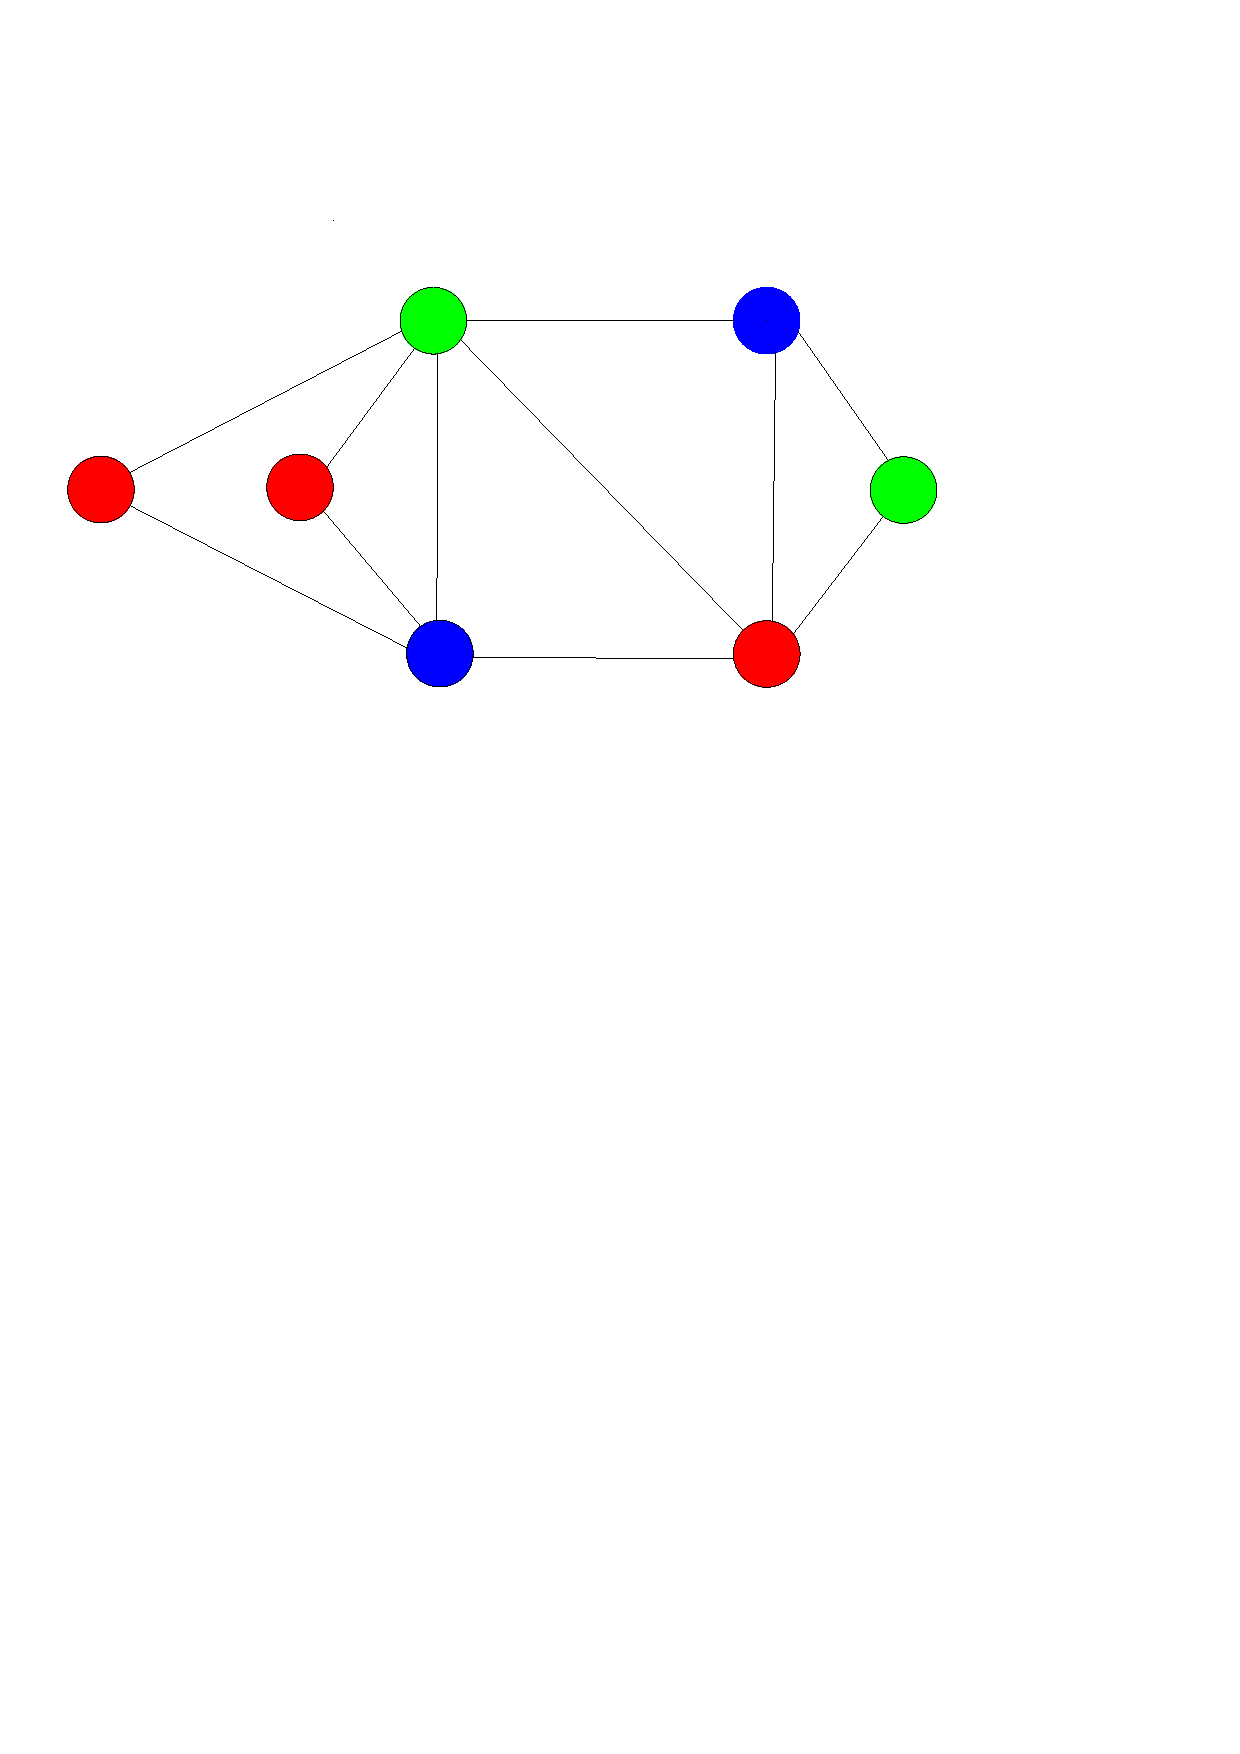
\includegraphics[width=\textwidth]{1/nodeColoring1.pdf}
  \end{minipage}
  \hfill
  \begin{minipage}[b]{0.49\textwidth}
    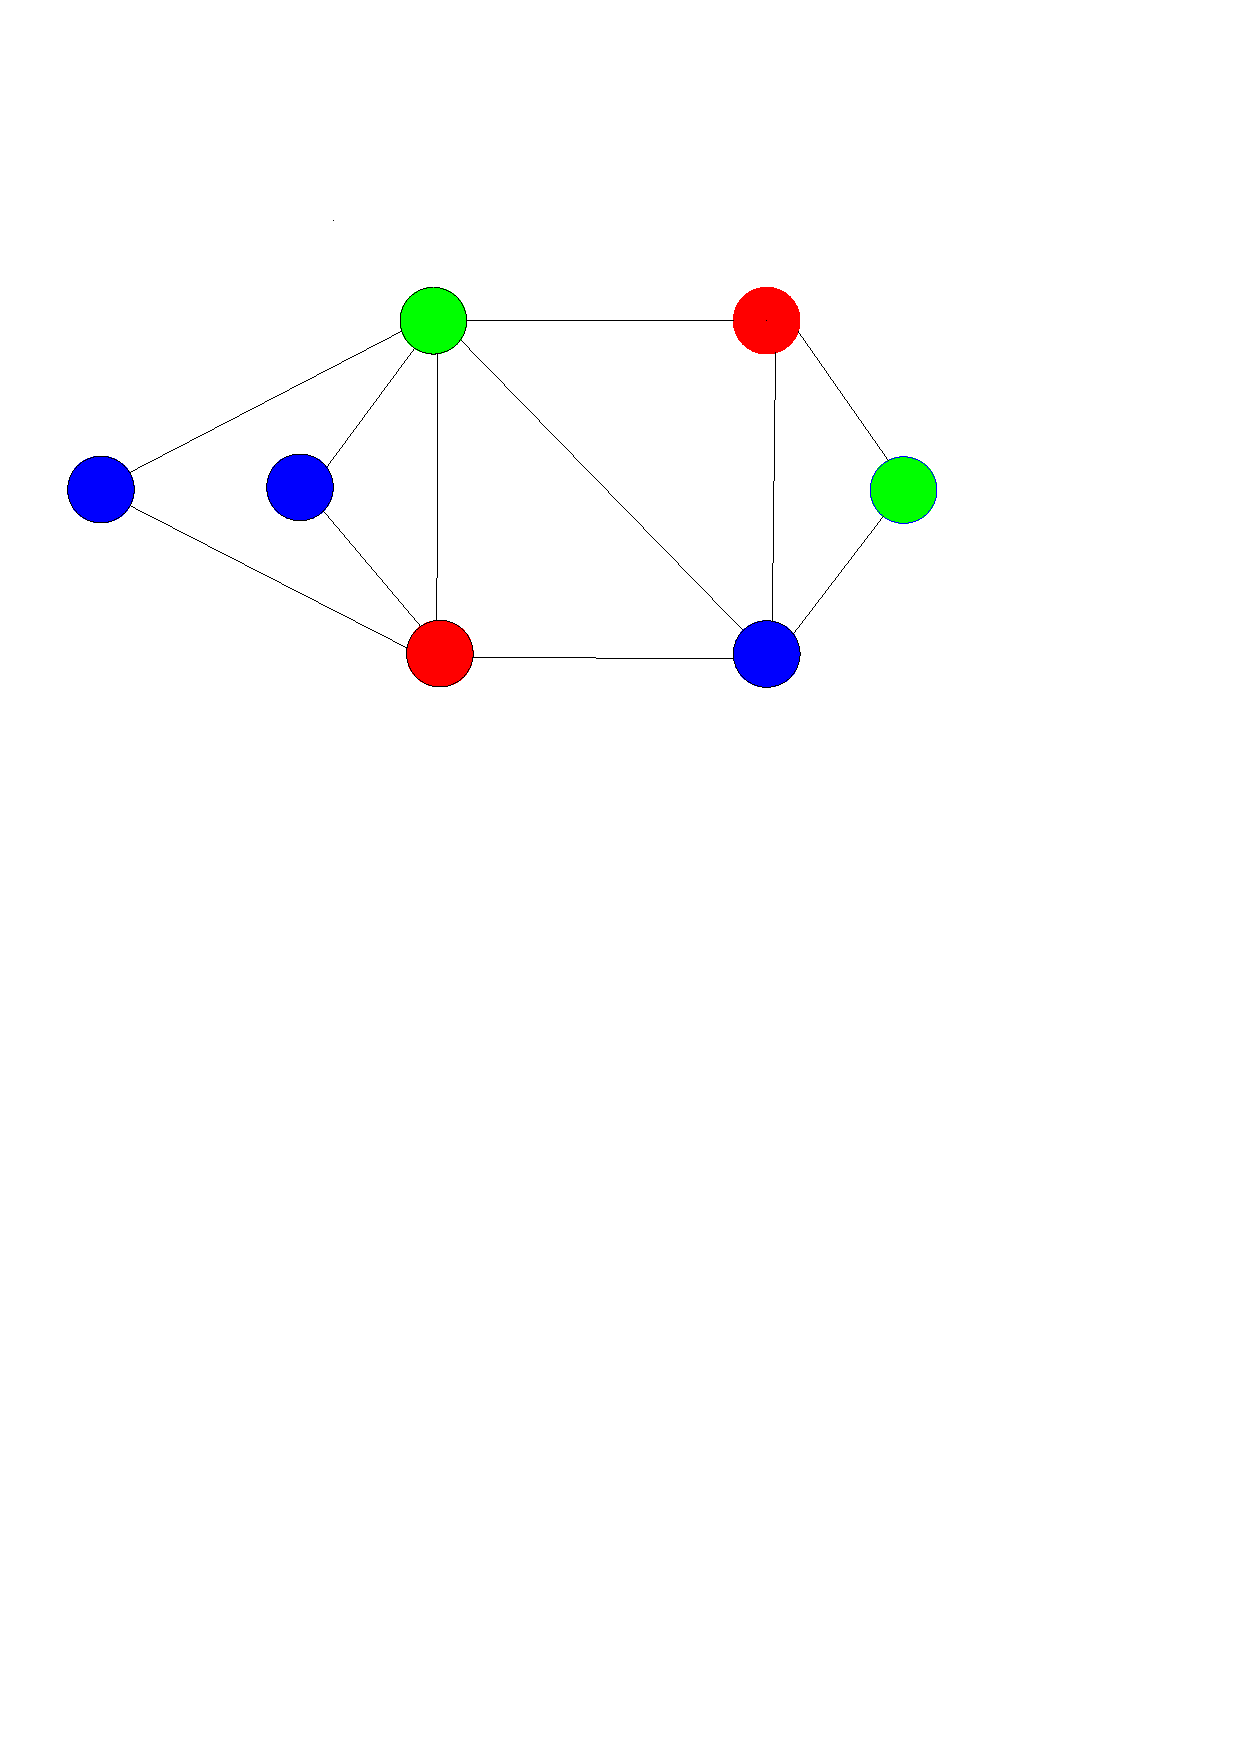
\includegraphics[width=\textwidth]{1/nodeColoring2.pdf}
  \end{minipage}
    \caption{Two 3-colorings of one graph. The chromatic number of this graph is 3.}

\end{figure}
The vertex coloring problem has many applications like computer register allocation \cite{chaitin1981register, chow1990priority} and printed circuit board testing \cite{garey1976application}. Two examples in our daily life are as follows.


1. \textbf{Timetable and scheduling} \cite{leighton1979graph,de1985introduction}

An Example of this application is to make an exam schedule. We suppose that several exams are going to be scheduled in a university. How to ensure the students do not have different exams in the same time slot? This problem can be seen as a vertex coloring problem, where the exams are represented by vertices in an undirected graph. Two exams involving the same student are connected with an edge. Here the minimum color number corresponds to a minimum number of time slots needed for all the exams.

\begin{figure}[h]
\centering
 \hbox{\hspace{7em}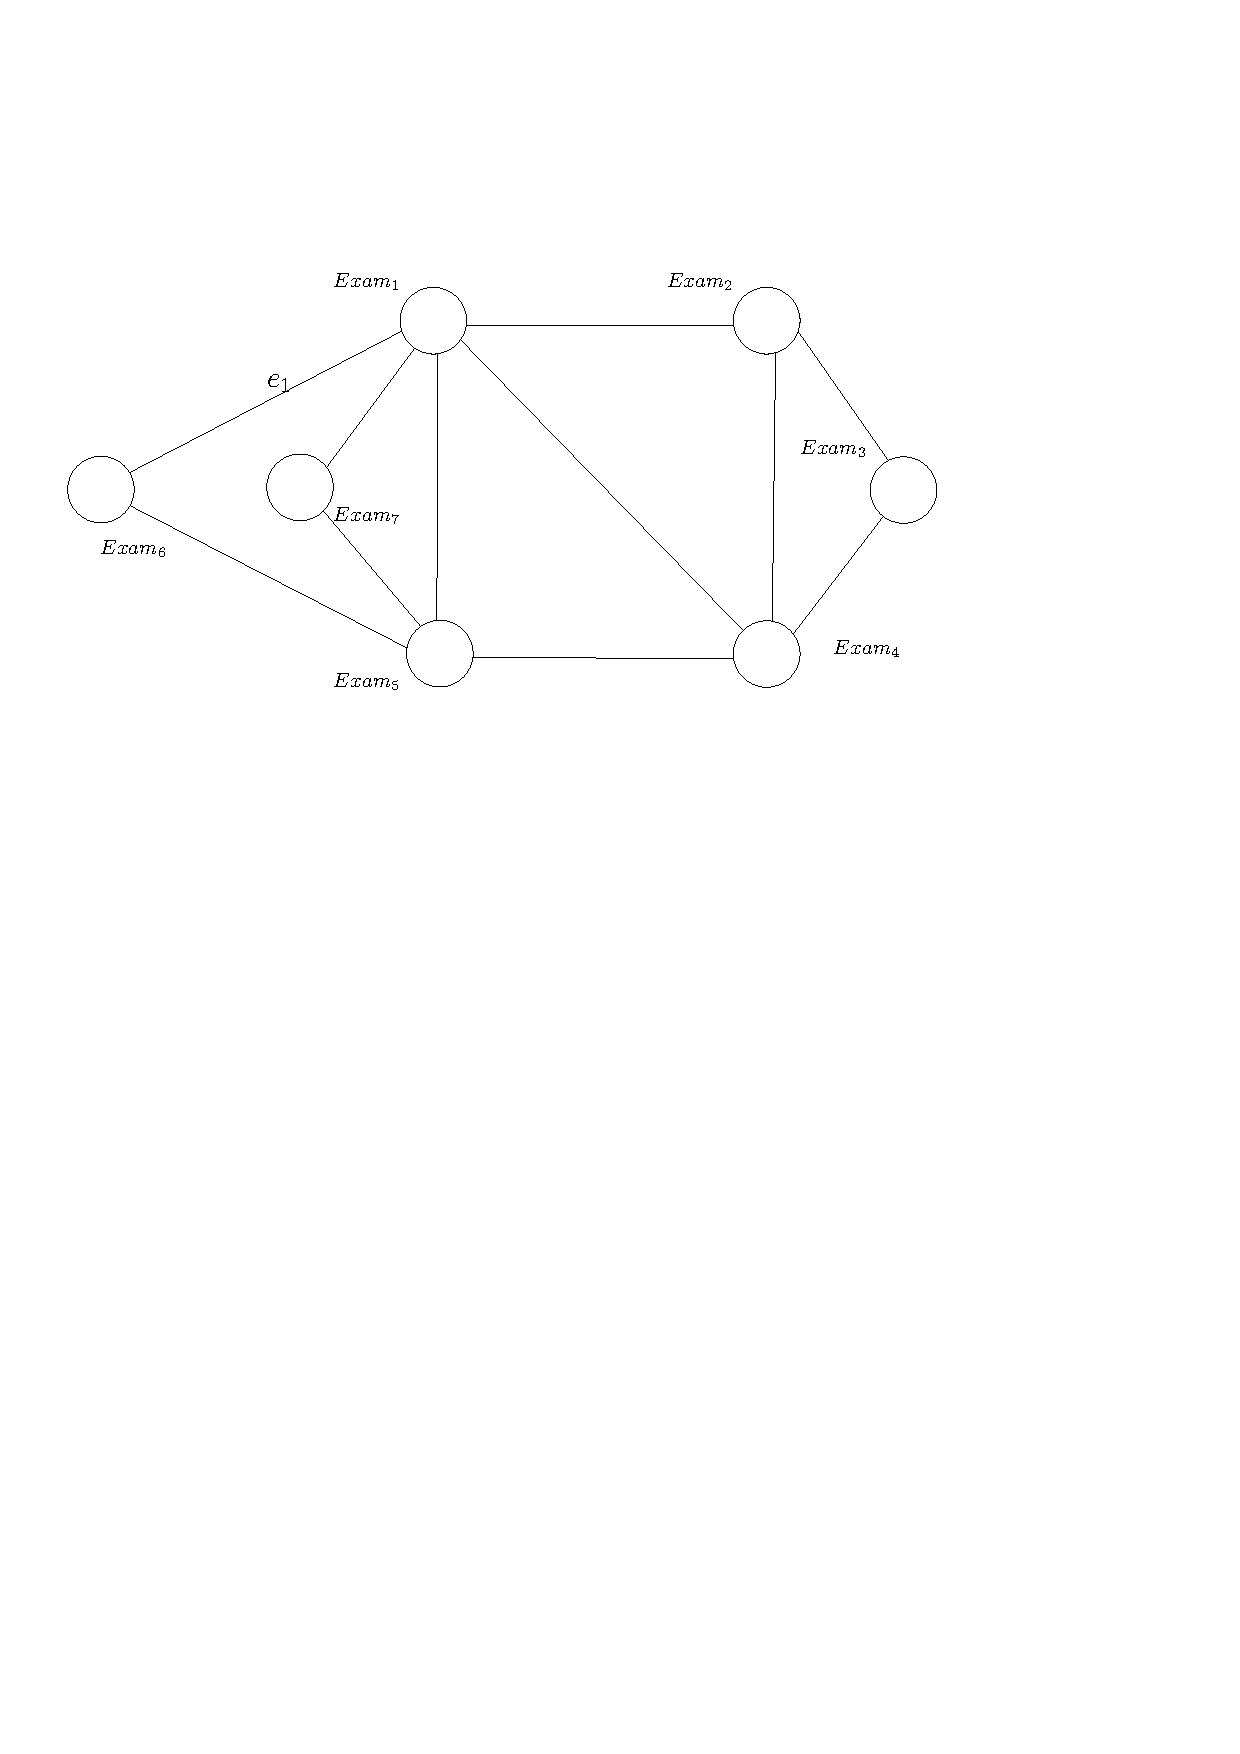
\includegraphics[scale=0.7]{1/timeTable.pdf}} 
  \caption{An example of the application in scheduling.   There are 7 exams in this example. The edge $e_1$ means some students take the 1st exam as well as the 6th exam.} 
\end{figure}
2. \textbf{Mobile Radio Frequency Assignment} \cite{gamst1986some}

Assigning frequencies to radio senders is also an example of the vertex coloring problem. The constraint is that senders received by the same location must use different frequencies. In a graph where the senders correspond to vertices, two senders have the same receiving location are connected with one edge. The aim is to color the senders with a minimum number of colors, which represent different frequencies.

\begin{figure}[h]
\centering
 \hbox{\hspace{7em}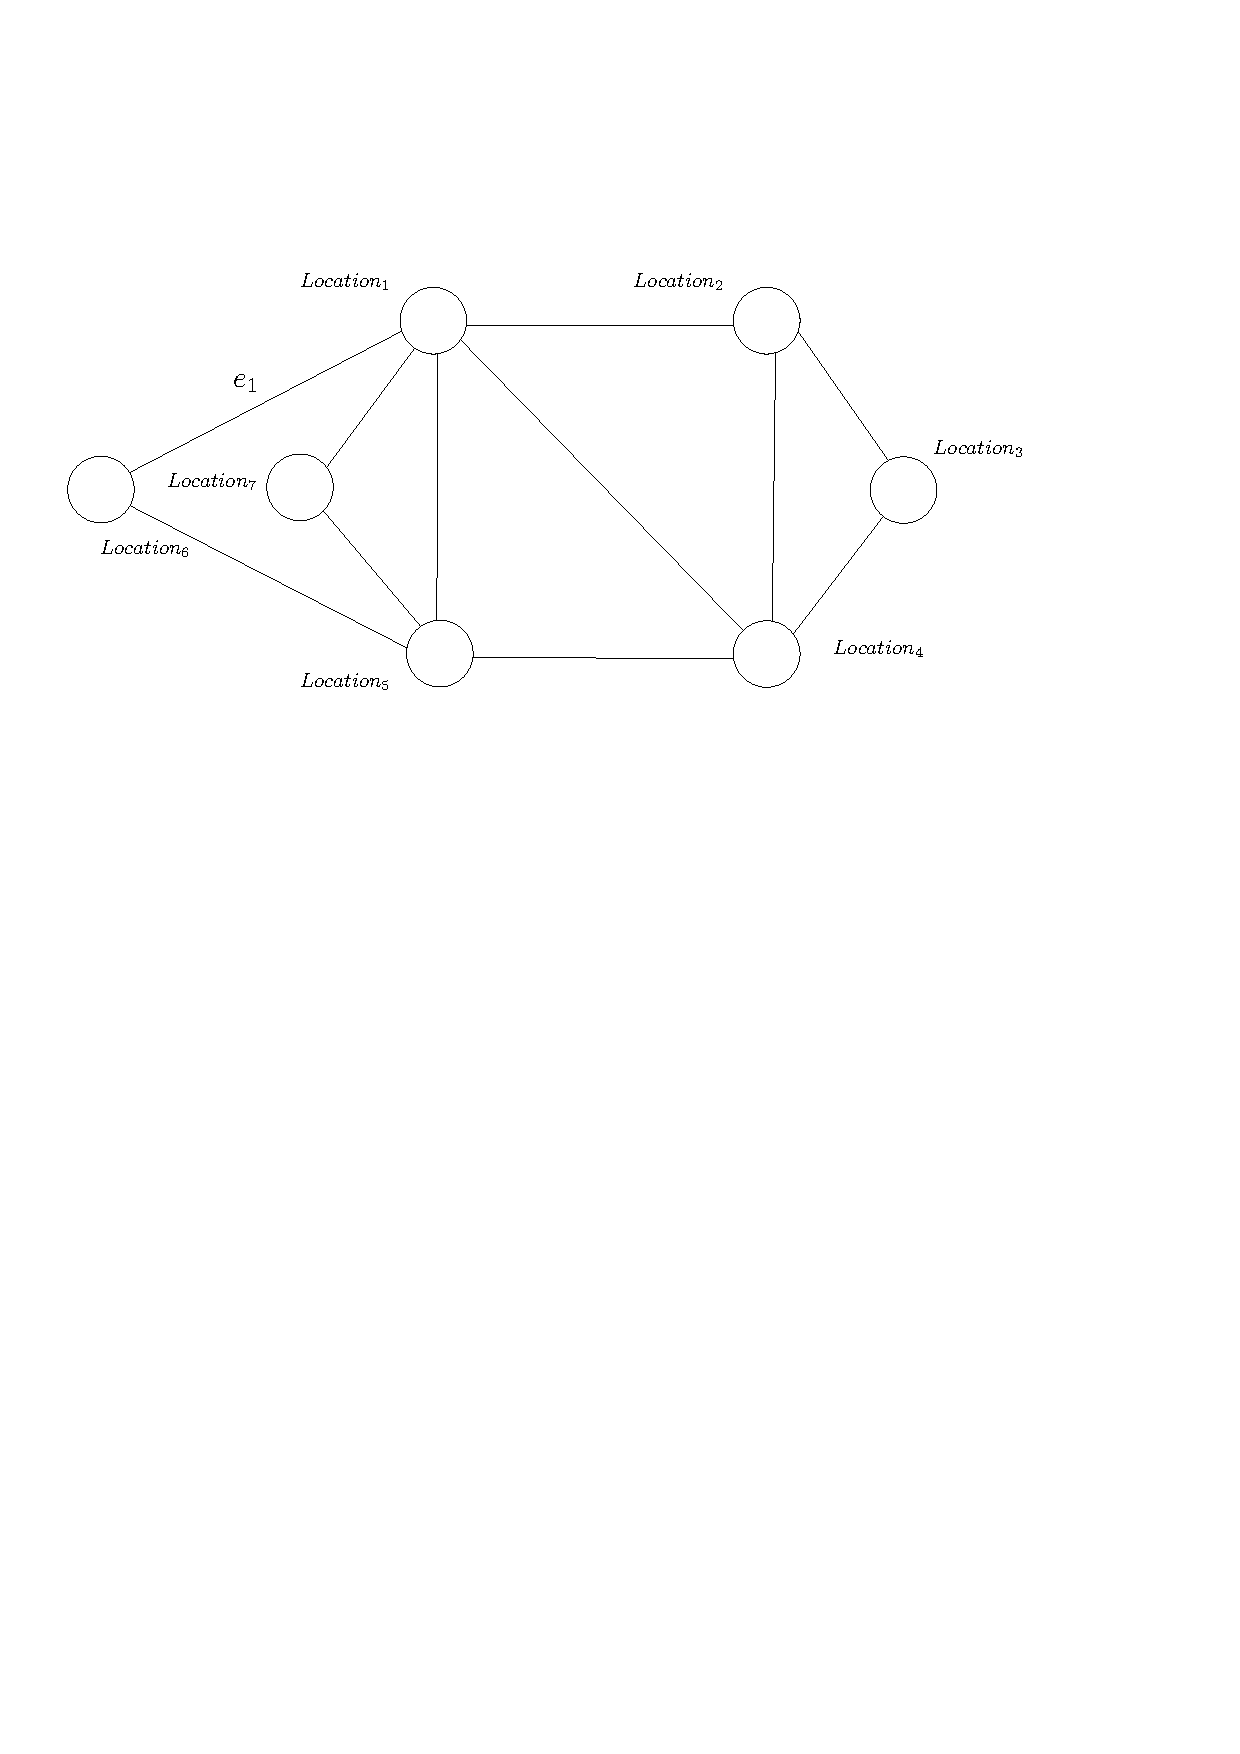
\includegraphics[scale=0.7]{1/Radio.pdf}} 
  \caption{An example of the application in frequency assignment. There are 7 locations in this example. The edge $e_1$ means a sender can be received by the 1st location as well as the 6th location.} 
\end{figure}

\subsection{Content}
The Graph coloring problem, as a well-known NP-complete problem \cite{gary1979computers}, has received a great deal of attention and different search methods have been developed \cite{minton1992minimizing, johnson1991optimization}. This thesis concentrates on solving the vertex coloring problem with one of the first local search algorithms Tabucol. Tabucol was proposed in 1987 by Hertz and de Werra \cite{hertz1987using}. As a very popular and well performing local search algorithm, Tabucol is often used as a subroutine in hybrid algorithms for solving GCP. This paper presents a GCP-solver which runs Tabucol iteratively on the same graph instance. In the first part of this thesis, different techniques to improve this algorithm are discussed. In the second part, we want to search the potential benefit of cooperative search, in which different agents run the same algorithm in parallel and exchange information in the search process. In this paper, Different kinds of cooperative work among agents are evaluated and compared. Some techniques turned out to be more efficient than the original search.
\section{Preliminaries}
\subsection{Definitions and Notations}
A \emph{\textbf{set}} is a container of unique elements. A set of 3 objects $a, b, c$ is written as $\{a ,b ,c\}$. The size of a set is the number of elements in the set.\\
A \emph{\textbf{graph}} $G$ = ($V,$ $E$) \cite{trudeau1993introduction} is a structure consisting of a finite set $V$ of vertices and a finite edge set $E \subseteq V \times V.$ Throughout the paper, we use $n =|V|, m =|E|$ if no other definitions are given. By $v_i$ we denote the $i$th element in $V$ and by $e_i$ the $i$th element in $E$. Based on the forms of the edges, there are two types of graphs: undirected graph and directed graph. In a \emph{\textbf{directed graph}}, the edge set contains ordered pairs of vertices, called arrows or directed edges. An edge $e = (u, v)\in E$ represents a connection from node $u$ to $v$. An \emph{\textbf{undirected graph}} is a graph in which edges have no orientation. The edge $e = \{u, v\}$ represents a connection between the vertices $u$ and $v$. It is identical to the edge $e'= \{v, u\}$. Two vertices are incident when they are connected by an edge. 
When an edge connects a vertex with itself, this edge is called a loop in the graph.

\begin{figure}[h!]
  \centering
  \begin{minipage}[b]{0.49\textwidth}
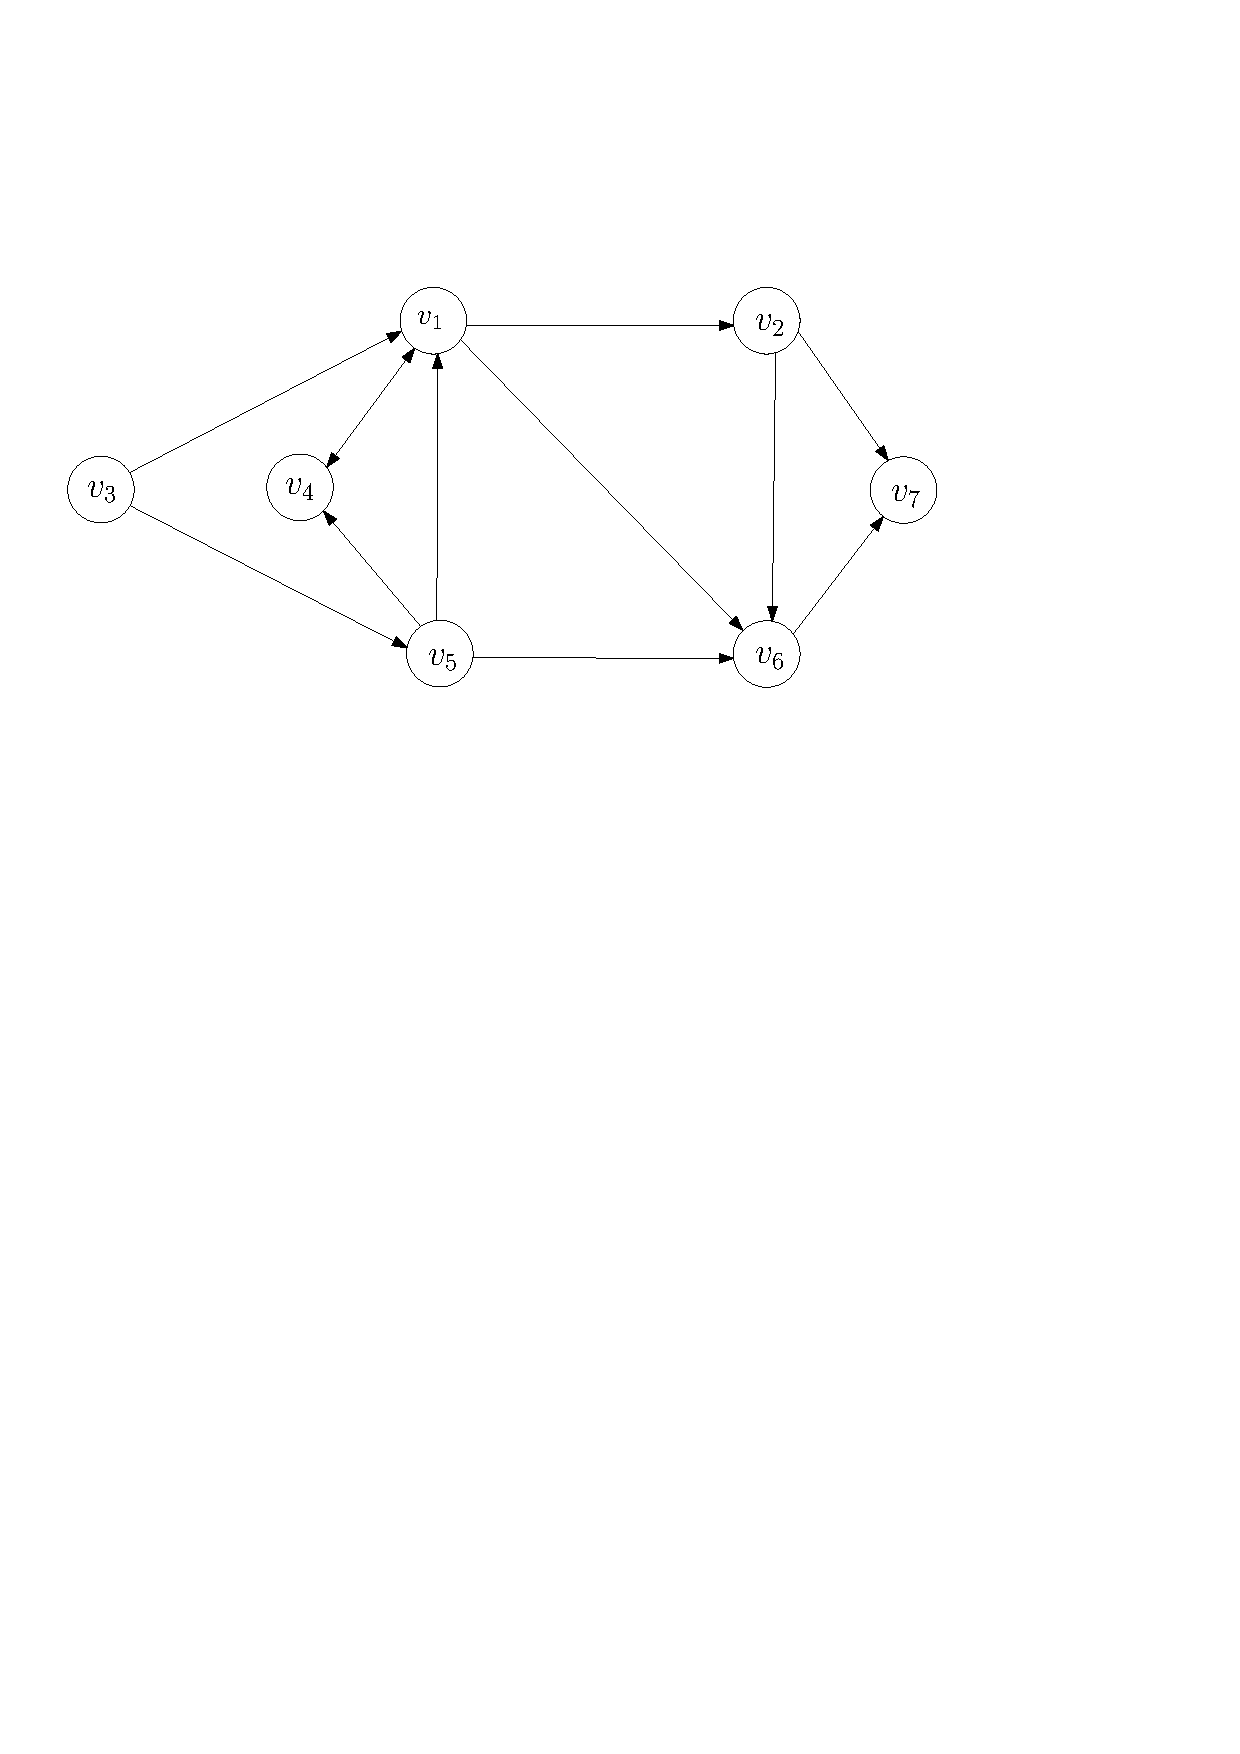
\includegraphics[scale = 0.5]{1/directedGraph.pdf}

  \end{minipage}
  \hfill
  \begin{minipage}[b]{0.49\textwidth}
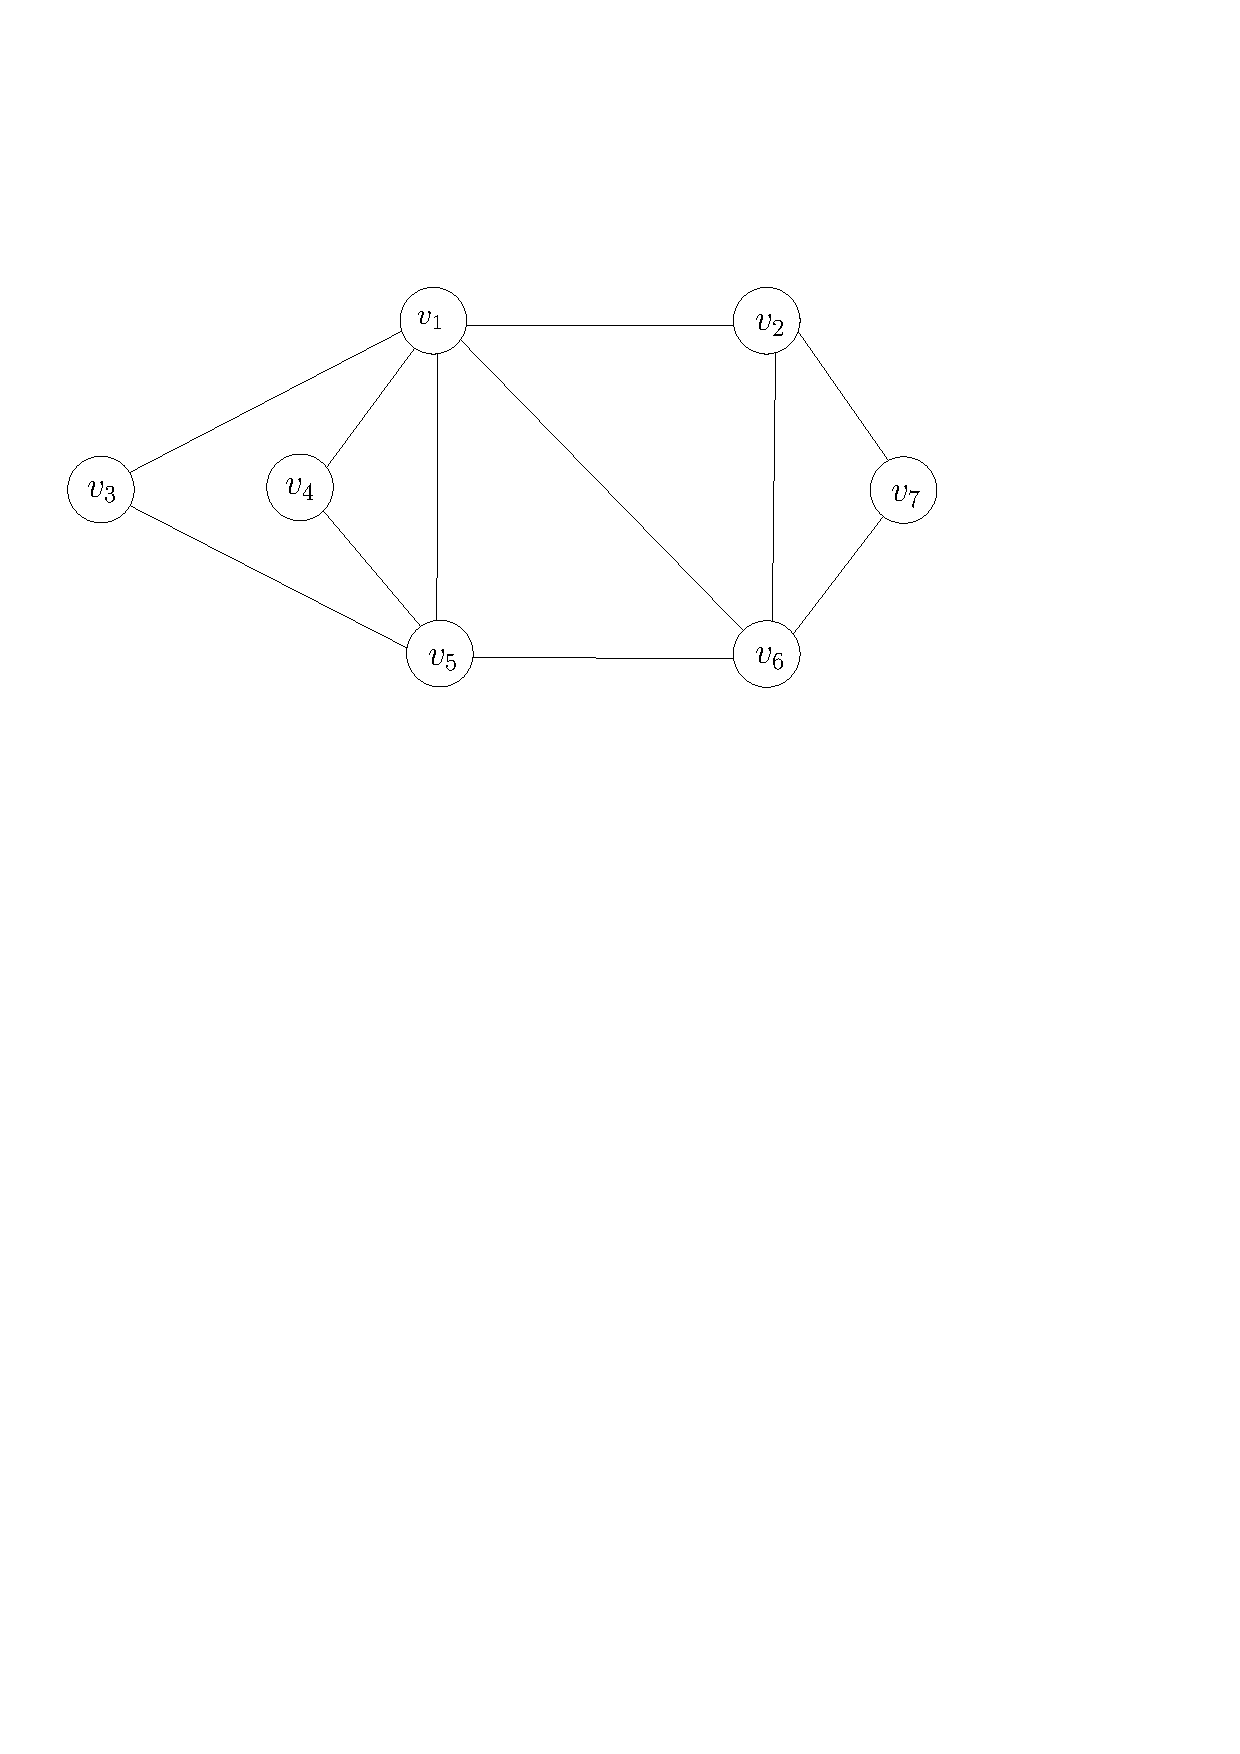
\includegraphics[scale = 0.5]{1/basicGG.pdf}

  \end{minipage}
    \caption{The figure above left  shows a directed graph. There are two edges between $v_1$ and $v_4$. The edge ($v_1, v_4$) is represented by an arrow from $v_1$ to $v_4$. The edge ($v_4, v_1$) is represented by an arrow towards $v_1$. An undirected graph is shown in the figure above right. There is one edge $\{v_1, v_4\}$ between $v_1$ and $v_4$. The edge $\{v_1, v_4\}$ is represented by a line connecting $v_1$ and $v_4$. The edge $\{v_1, v_4\}$ is equal to the edge $\{v_4, v_1\}$.}
\end{figure}

\emph{\textbf{The graph coloring problem}} (\emph{\textbf{GCP}})\label{Graph coloring problem}
 deals with the assignment of labels called ``colors'' to elements of a graph subject to certain constraints.\\
When used without any qualification, a coloring of a graph is almost always a proper vertex coloring, 
A vertex coloring of a graph is a function $c$: $V\rightarrow \{1...k\}$. The coloring with $k$ colors is called a \emph{\textbf{k-coloring}}. The value $c(v_i)$ of a vertex $v_i$ is called the color or the index of the color of the vertex $v_i$. A coloring is a \emph{\textbf{legal coloring}} when no two adjacent vertices share the same color. Otherwise, when an edge connects two same-colored vertices in a coloring, the edge is called a \emph{\textbf{conflicting edge}}. A coloring with at least one conflicting edge is an \emph{\textbf{illegal coloring}}. The \emph{\textbf{conflict number}} $f(c)$ of a coloring $c$ is the number of conflicting edges in the coloring. In other words, $f(c)=\sum |E_i|$, $E_i = \{(v,w)\in E,c(v)= c(w)= i\}$.
The \emph{\textbf{k-GCP}} problem is to determine whether a legal $k$-coloring exists for the graph or not. The \emph{\textbf{GCP}} problem is to determine the smallest $k$, such that the graph can be colored using $k$ colors without conflicts. This lower bound $k$ is called the \emph{\textbf{chromatic number}} of G, denoted by $\chi(G)$.
\begin{figure}[h!]
  \centering
  \begin{minipage}[b]{0.49\textwidth} 
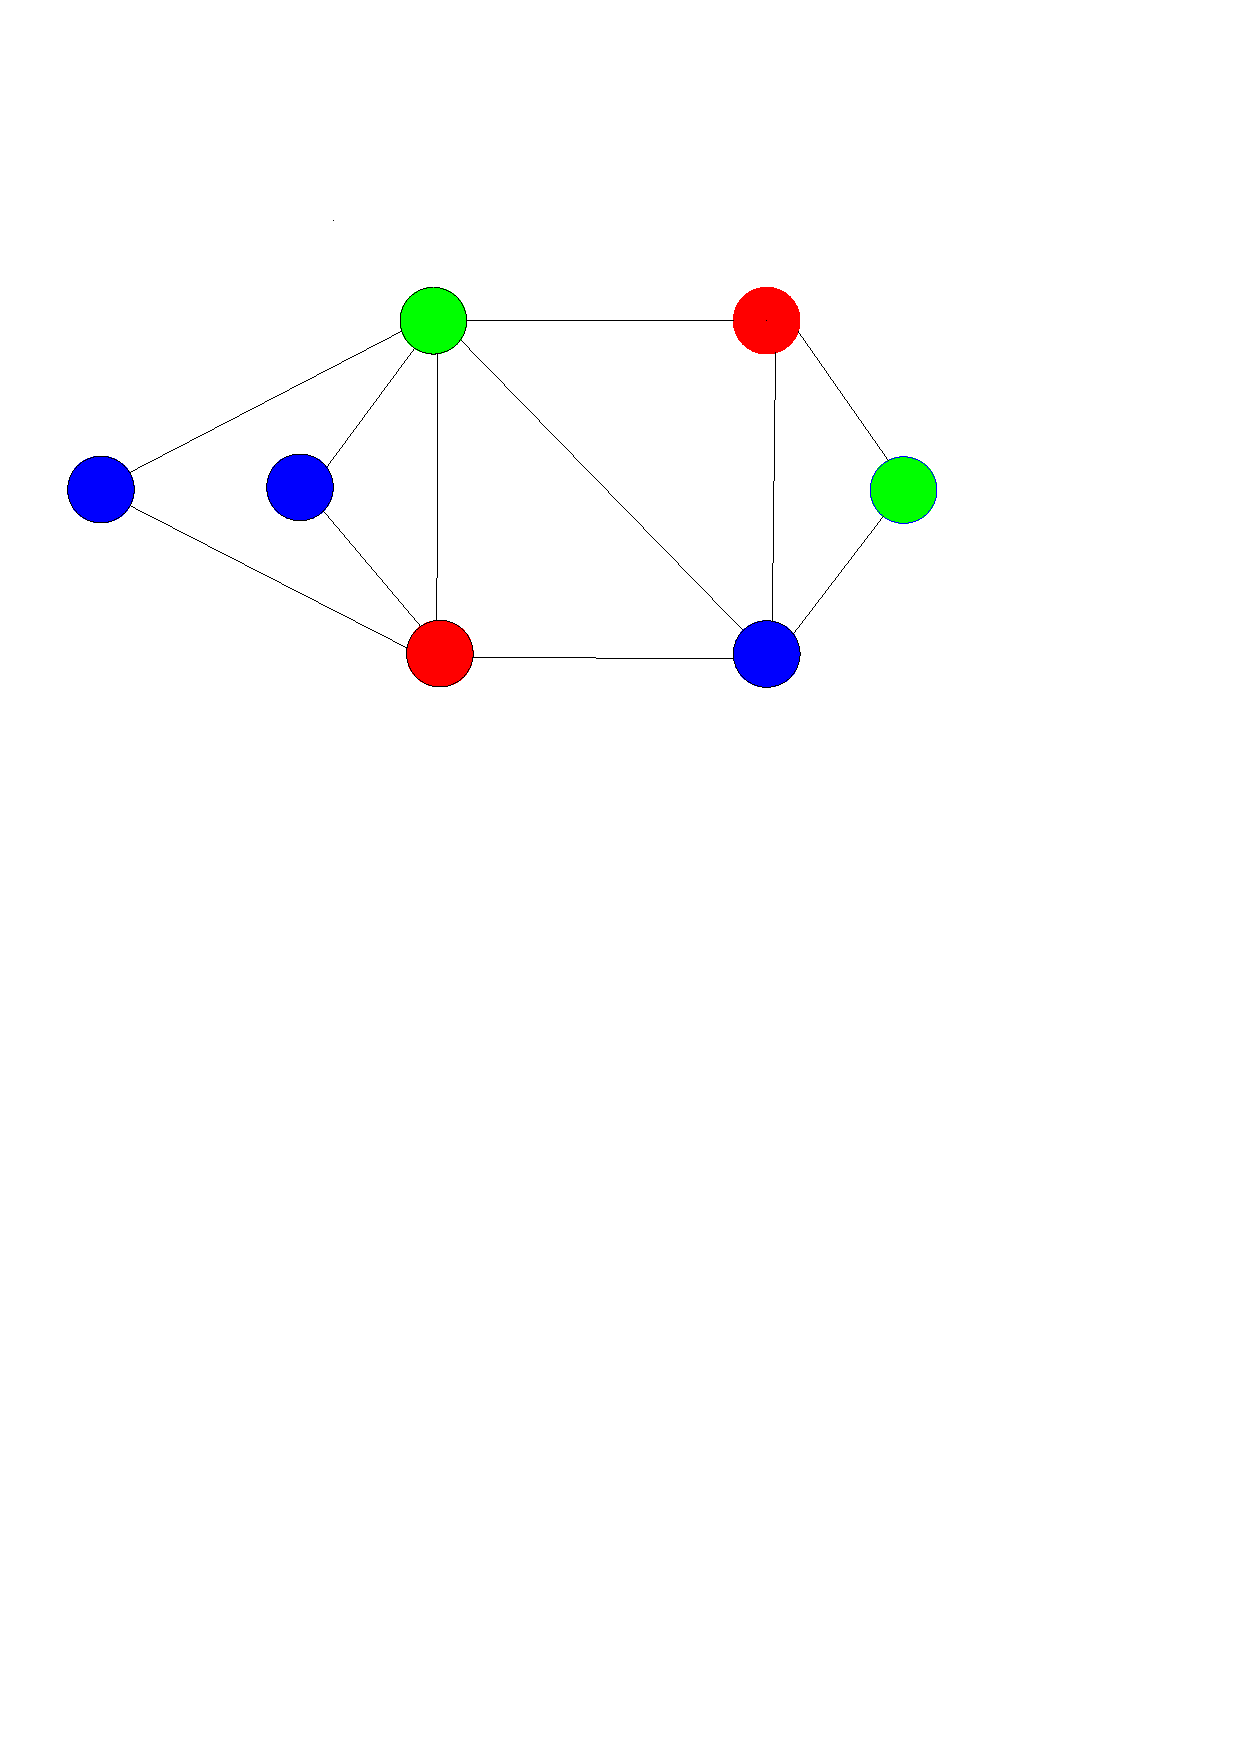
\includegraphics[scale = 0.5]{1/nodeColoring2.pdf}
  \end{minipage}
  \hfill
  \begin{minipage}[b]{0.49\textwidth}
  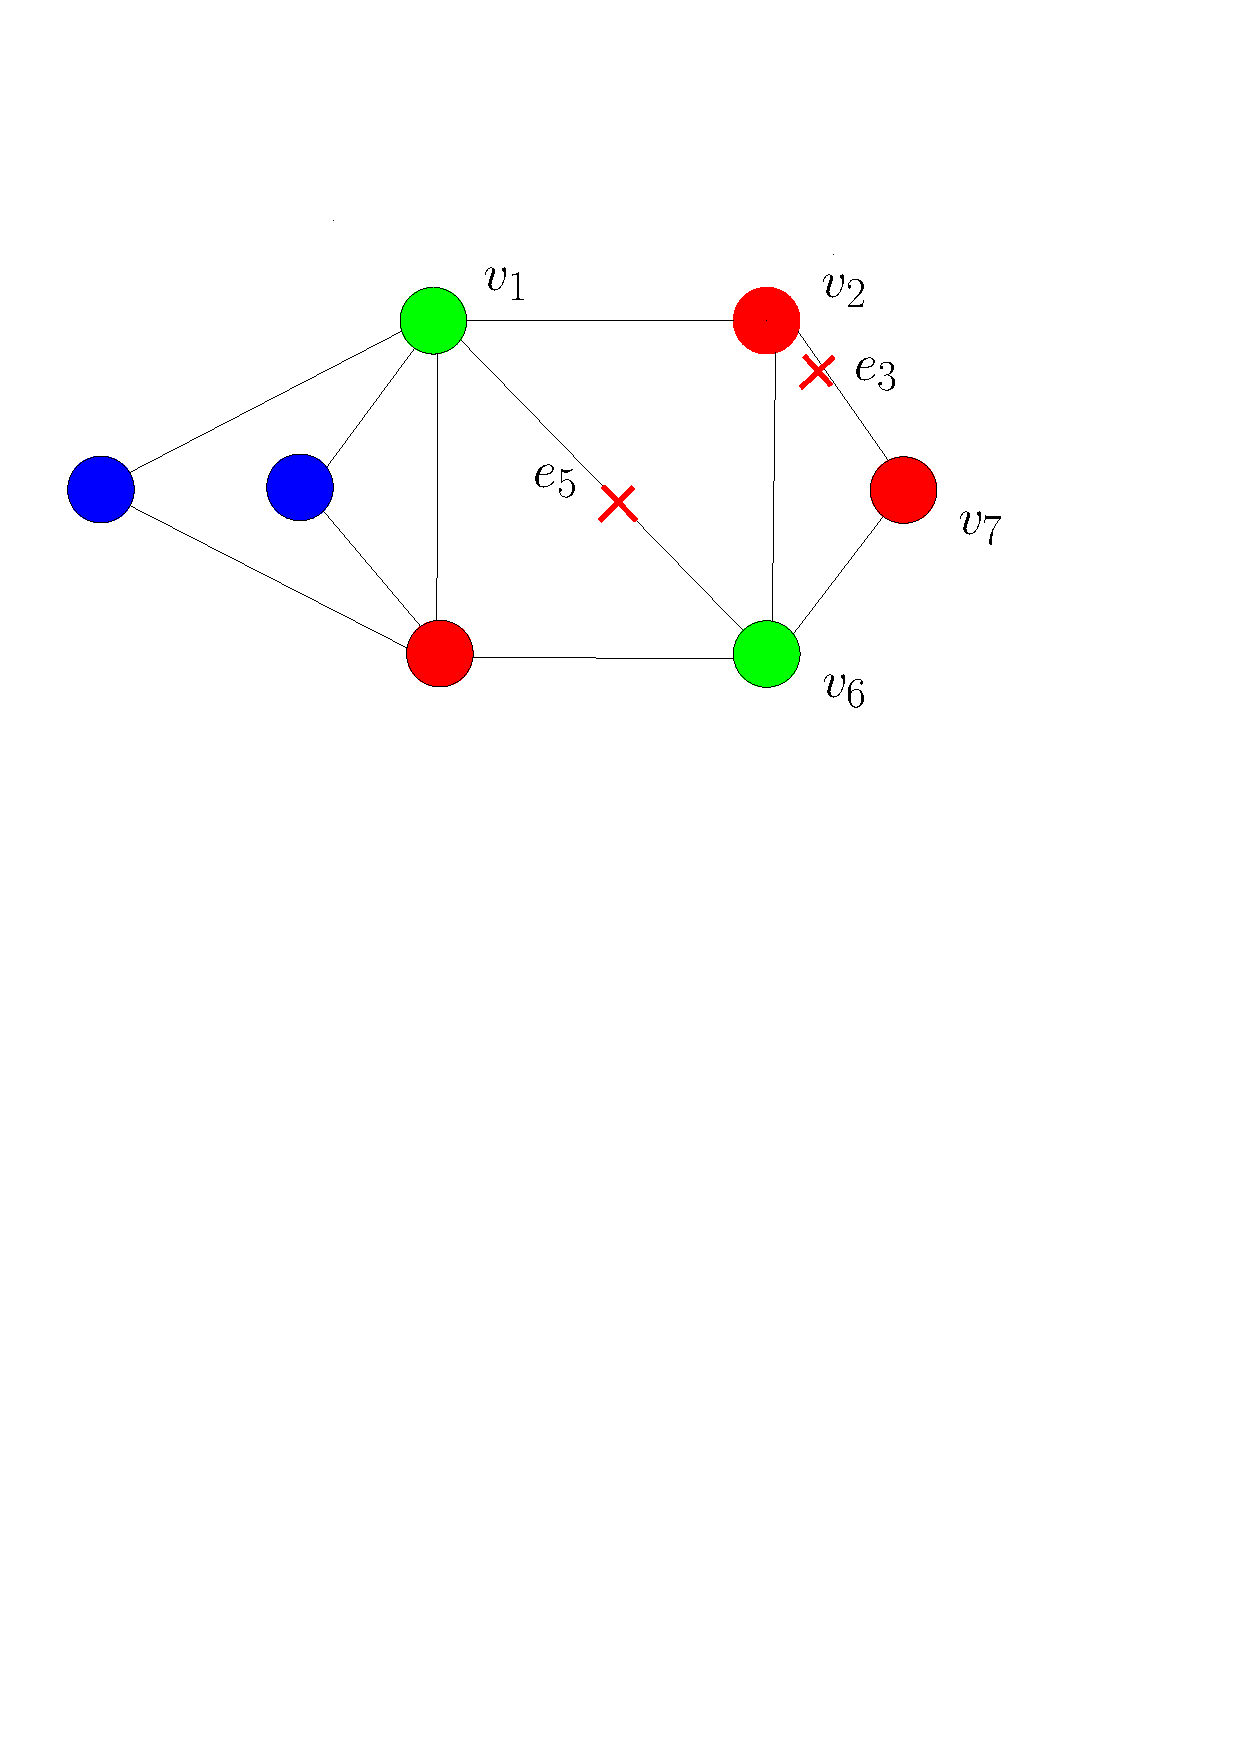
\includegraphics[scale = 0.5]{1/conflict.pdf}
  \end{minipage}
  \caption{
  The figure left above shows a 3-coloring example. This is a legal coloring without conflicting edges. The chromatic number of the graph $\chi(G)$ is thus 3. The figure right above is an illegal 3-coloring with conflict number 2. A Conflicting edge $e_5$ connects two green-colored vertices $v_1$ and $v_6$. The conflicting edge $e_3$ connects two red-colored vertices $v_2$ and $v_7$.}\label{Figure 6}
\end{figure}\\

\emph{\textbf{Neighboring coloring}}\\
A neighboring coloring $c'$ of a coloring $c$ is a coloring differs from $c$ in the color of one vertex $v$.\\
$c(w)$ = $c'(w)$ for $w \neq v$; $c'(v) \neq c(v)$.

\emph{\textbf{Local search}}\\
A local search starts with an initial illegal coloring. To reach a neighboring coloring, the local search makes local changes to its current coloring iteratively, hence the name local search. Usually, each coloring has more than one neighbors. The decision which neighbor will be reached in next step depends on some criterion. Local search is widely used in hard problems such as the traveling salesman problem \cite{stutzle1997max} and the boolean satisfiability problem \cite{zhang2004configuration}.

\begin{figure}[h!]
\centering
 \hbox{\hspace{12em} 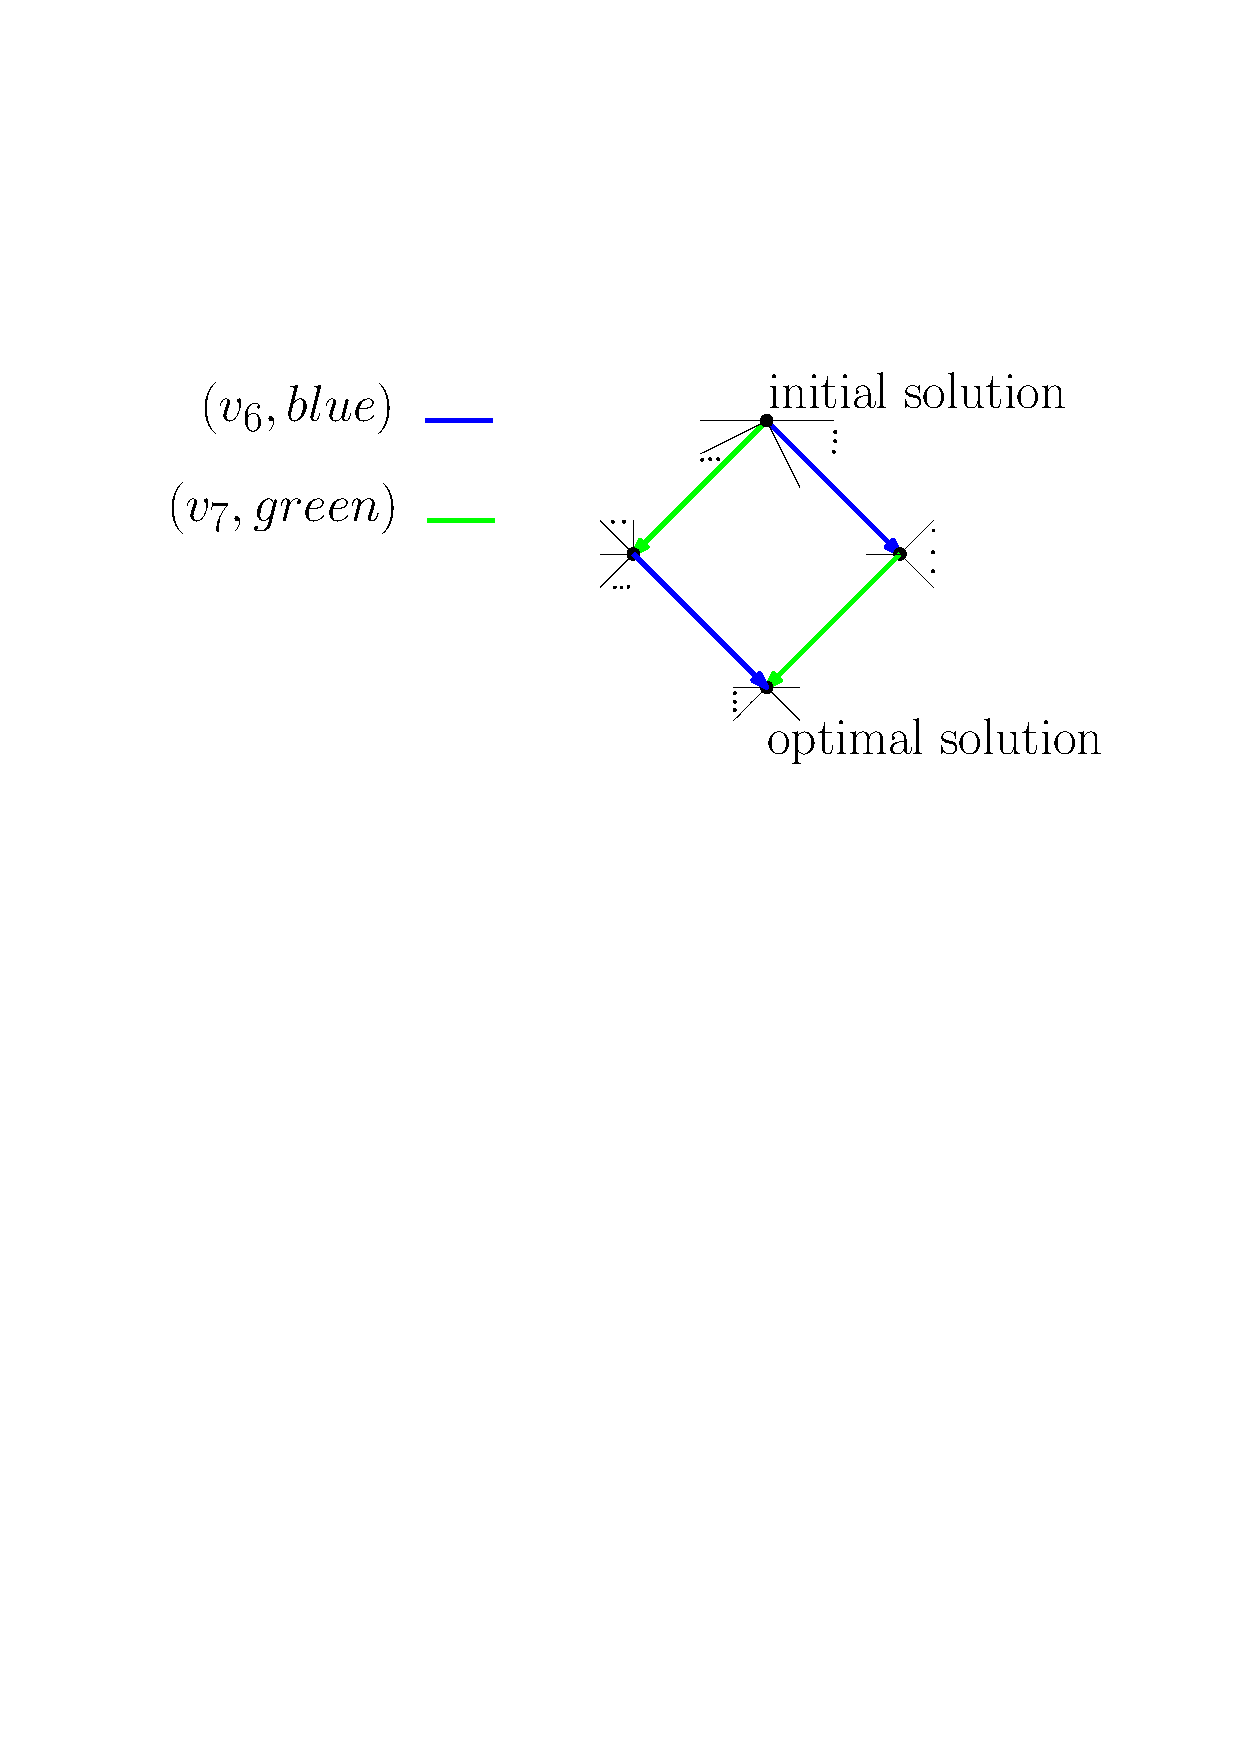
\includegraphics[scale = 0.6]{1/localsearch.pdf}}
 \caption{Figure 10 is an example of a local search in coloring problem. Colorings are represented by nodes in a net. The search changes one color iteratively to improve the coloring to have fewer conflicts. The initial coloring of this Example is the right coloring in Figure \ref{Figure 6}. The optimal coloring is the coloring shown left in Figure \ref{Figure 6}. Blue edges represent changing $v_6$ to blue (read from the upper node to the lower node). Green edges represent changing $v_7$ to green.}
\end{figure}


\emph{\textbf{Tabu search}}\\
Local search methods move in a neighborhood and have a tendency to get stuck in suboptimal regions. Tabu search created by Fred W. Glover in 1986 \cite{glover1986future} and formalized in 1989 \cite{glover1989tabu1}\cite{glover1990tabu2}.
The search trace is recorded in the process. The recently reached neighboring colorings are marked as tabu colorings. The tabu colorings will not be touched in the further search to discourage getting stuck in a region.

\emph{\textbf{Hash table/map}} \cite{cormen2009introduction}\\
A hash table or a hash map is a directory, which maps keys to values. With the help of a hash function, the hash table is advantageous in respect of speed. Specifically, the overall complexity of common operations such as search, insertion or deletion is $O (1)$.


\begin{figure}[h]
\centering
 \hbox{\hspace{12em} 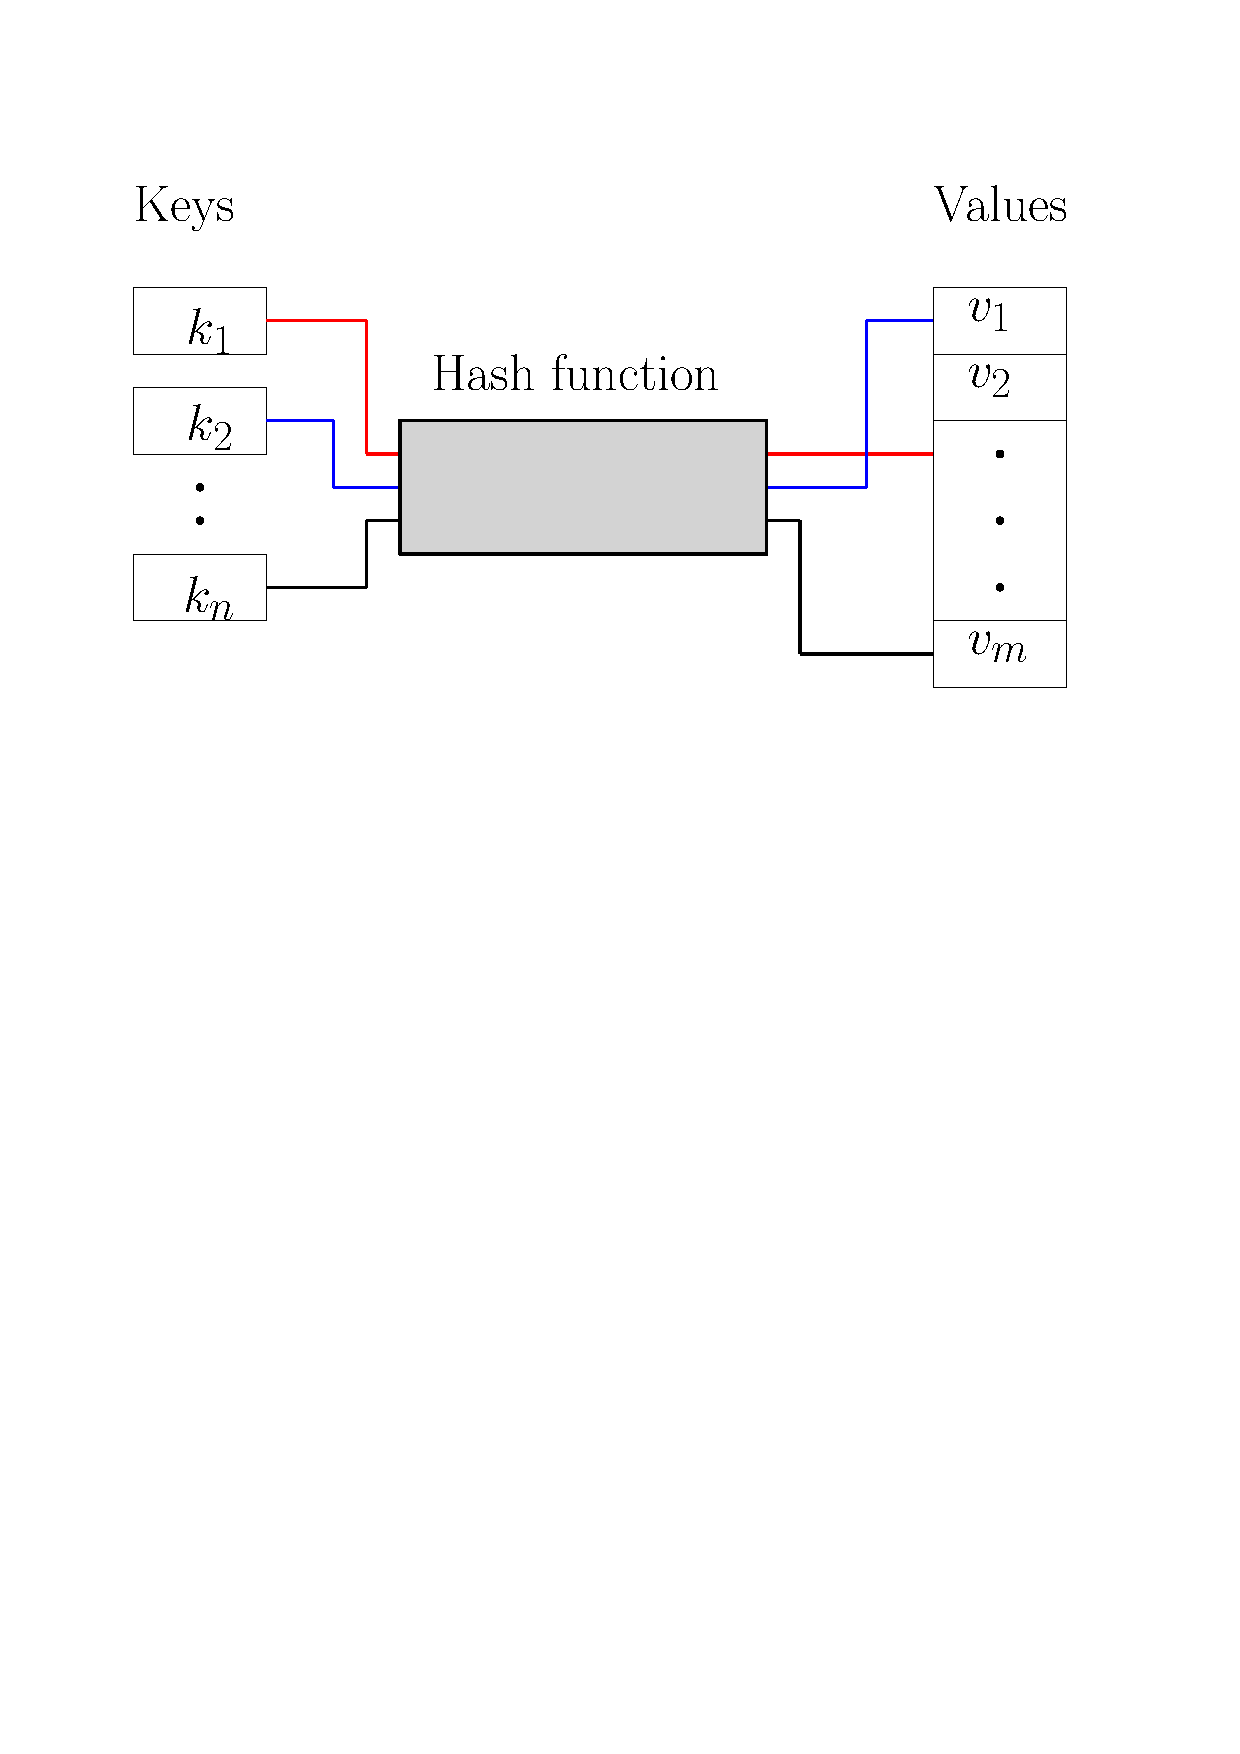
\includegraphics[scale = 0.6]{1/hashTable.pdf}}
 \caption{Hash table}
 A hash function is similar to a directory, which maps keys to stored values.
\end{figure}

\emph{\textbf{Matrix}}\\
A $p\times q$ matrix is a function $f_A: \{1...p\}\times\{1...q\}\rightarrow R$. A Matrix is normally represented by an ordered scheme $A$ with $p$ rows and $q$ columns. The value of the $i$th row and the $j$th column in a scheme $A$ is denoted by $A_{ij}$ and is equal to the function value $f_A(i, j)$.
\begin{figure}[h!]
\centering
 \hbox{\hspace{12em} 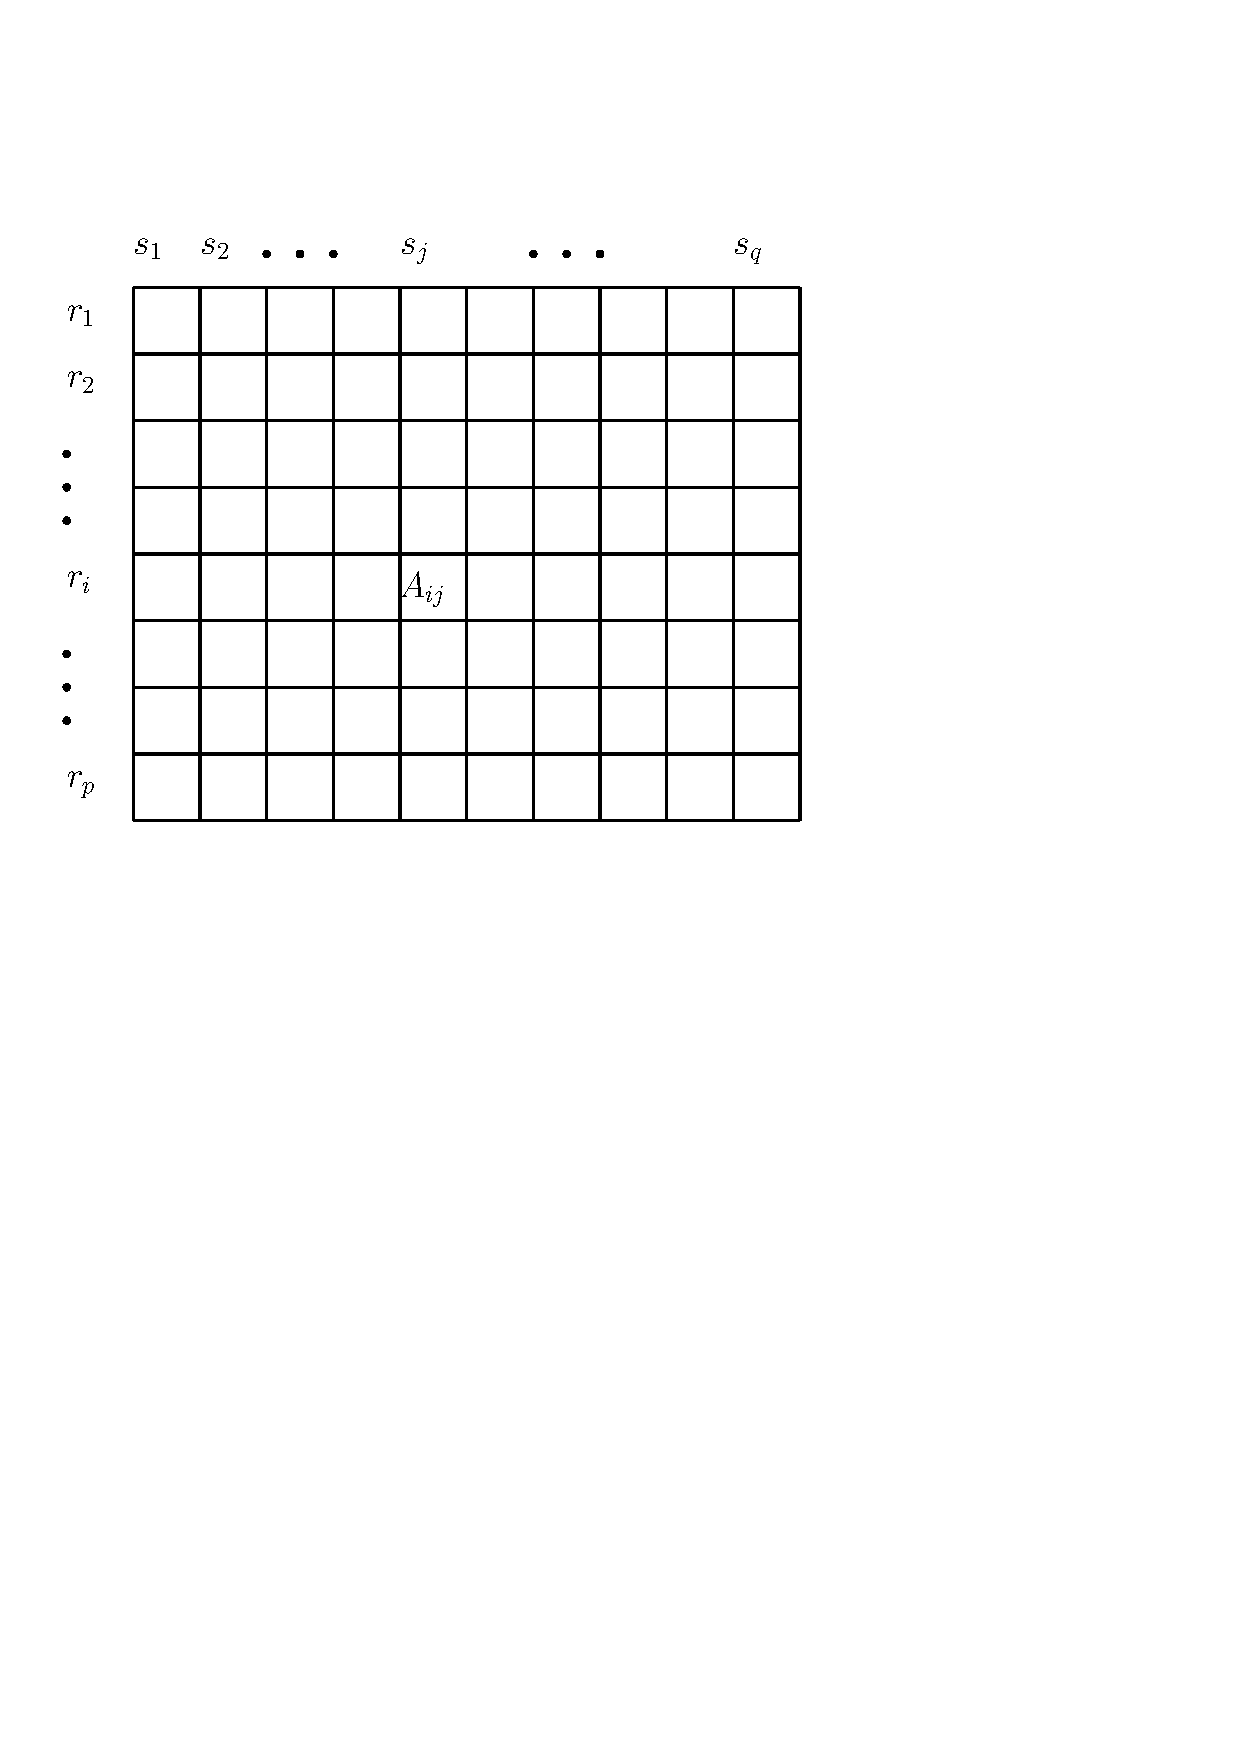
\includegraphics[scale = 0.6]{1/matrix.pdf}}
 \caption{A $p\times q$ matrix}.
\end{figure}

\emph{\textbf{Queue}}\\
The queue is an abstract data structure with two operations: enqueue where an element is pushed in the collection and dequeue where the element added in the collection earliest and not removed yet is removed from the queue.
The elements come in the queue in one end and come off from another end. This policy is called FIFO (first in-first out).
\begin{figure}[h!]
\centering
 \hbox{\hspace{12em} 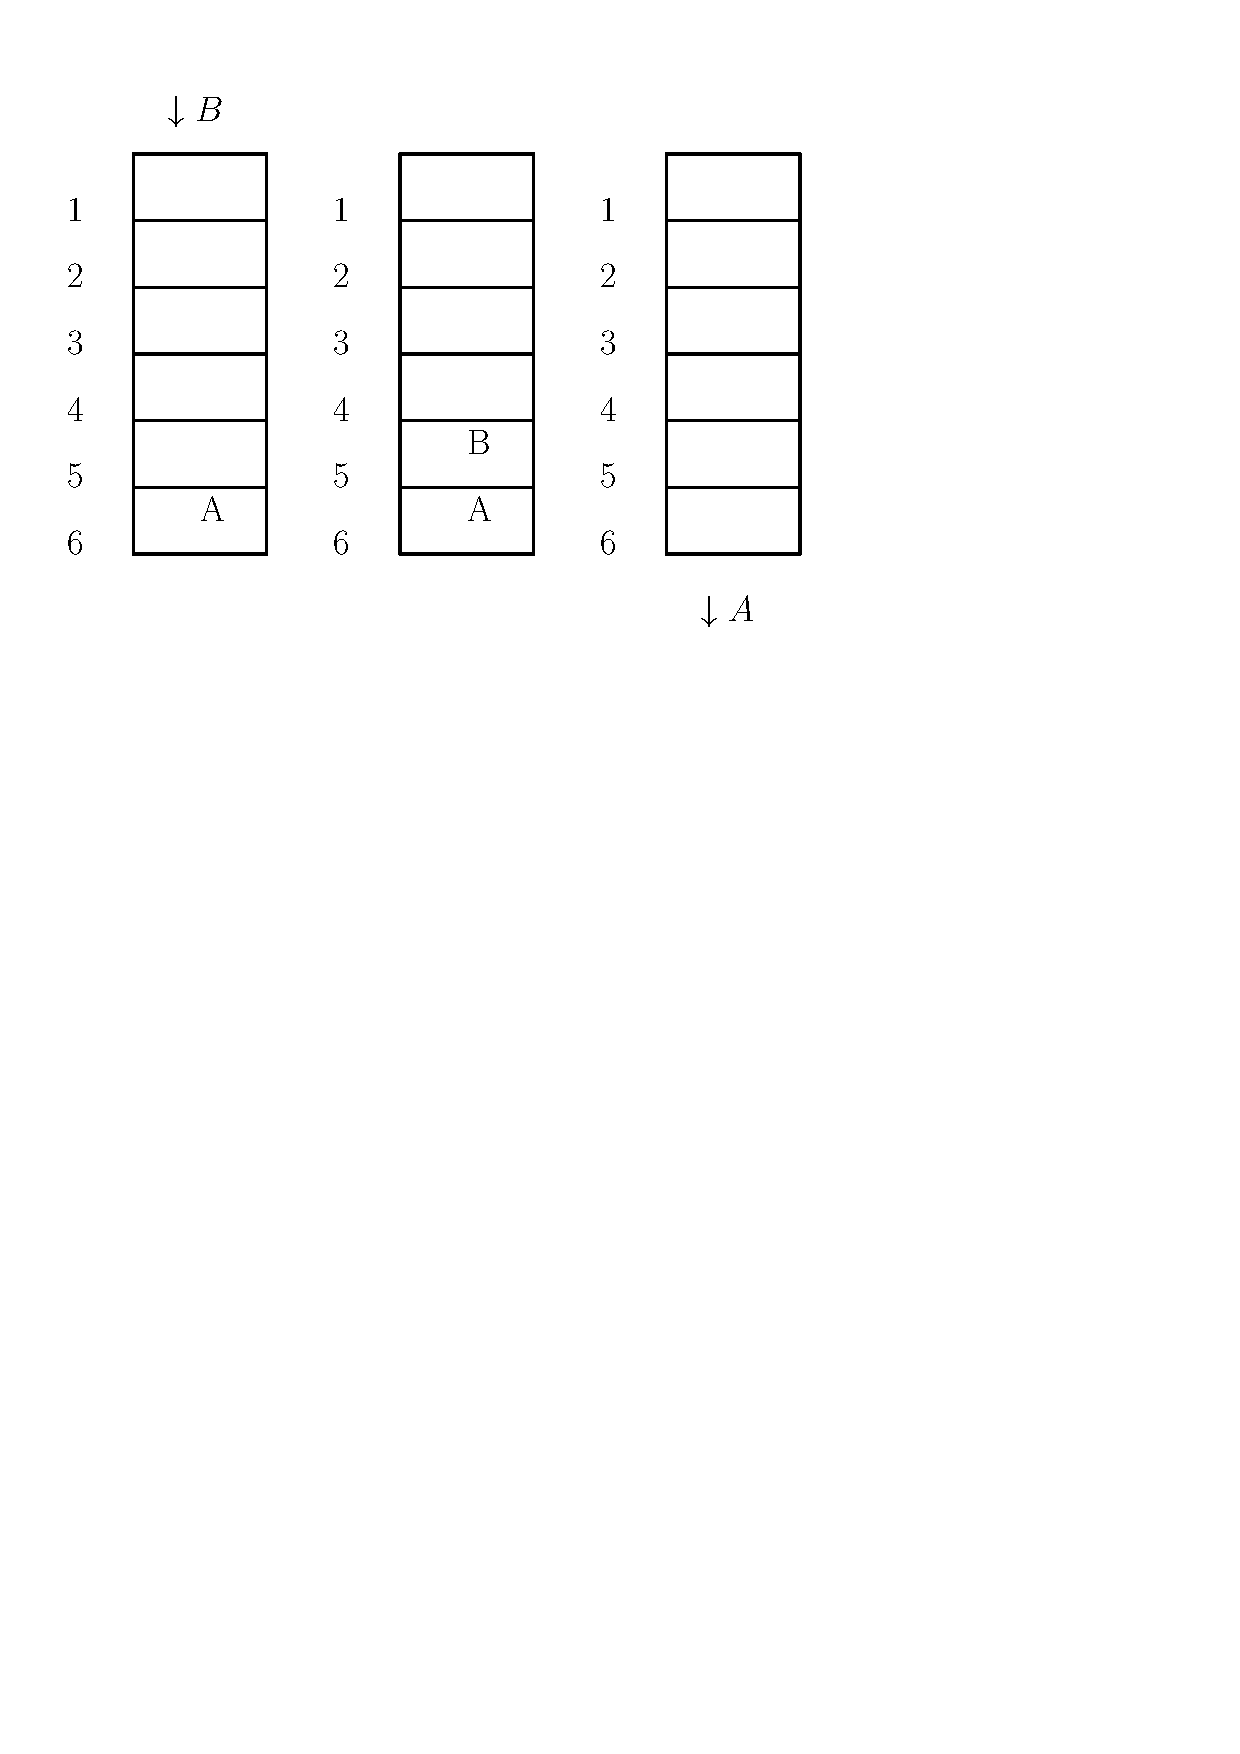
\includegraphics[scale = 0.6]{1/queue.pdf}}
 \caption{Enqueue and dequeue under FIFO policy}.
\end{figure}

\subsection{The algorithms for comparison}
\label{comparison}
To evaluate the performance of our algorithm, three other algorithms for solving the GCP are used for a comparison with our algorithm (see Experiment 9 in \ref{sec:Experiment 9}). The three algorithms for comparison are DSATUR, Trick's algorithm, and PASS.\\

\emph{\textbf{DSATUR}} \cite{brelaz1979new}\\
DSATUR is a sequential vertex coloring algorithm to color the vertices in turn until each vertex is colored. This greedy coloring algorithm maximizes saturation degree that is the number of colors assigned to its adjacent vertices. If multiple vertices with maximum saturation degree exist, the one with the maximal degree in the uncolored subgraph is chosen. The DSATUR algorithm assigns the smallest possible color to the chosen vertex in each step.
There are some variations of DSATUR. Two examples are Trick's algorithm and PASS.

\emph{\textbf{Trick's algorithm}} \cite{Trickalgorithm}\\
A clique of the graph is a set of mutually adjacent vertices. Naturally, to color, a clique of $k$ vertices needs at least $k$ different colors. The Trick algorithm makes use of this relationship of cliques and coloring. The algorithm finds and colors the large cliques in the graph and then applies the DSATUR algorithm on the uncolored subgraph.

\emph{\textbf{PASS}} \cite{san2012new}\\
The tie breaking strategy of the DSATUR algorithm is to choose the vertex with the maximum degree if multiple vertices with maximum saturation degree exist. The PASS algorithm is a DSATUR-based algorithm with a different tiebreaking strategy. The tiebreaking strategy aims to color that candidate vertex first, which has the least number of admissible colors. This strategy is based on the observation, that the vertices with small admissible colors in the current step are likely to require a new color in the further search.\\

We cannot find any source code for Tabucol-based algorithms. We chose these tree DSATUR-based exact coloring algorithms for comparison because these algorithms are much employed with their simplicity and efficiency.
\subsection{The Tabucol algorithm}
\emph{\textbf{Tabucol}} was introduced in 1987 by Hertz and de Werra \cite{hertz1987using}. Since then, some modifications are introduced to the original tabu search. The version I use in this paper is based on the paper by Galinier P \cite{galinier2006survey}. \\
The algorithm Tabucol is a tabu search to solve the k-GCP. Formally, for a Graph $G = (V, E)$, Tabucol wants to find a function $c: V\rightarrow\{1..k\}$ with constraint: $\forall$ $\{u, v\}\in E, c(u)\neq c(v)$. An evaluation function $f$ measures the number of conflicting edges in a coloring. In other words, the Tabucol is to determine, whether a $k$-coloring $c$ exists with $f(c) =0$. The local search will start from an initial $k$-coloring $c$. Changing the color of one vertex $v$ to color $i$ ($c(v) \neq i \land \exists$ $ w \in V, c(w) = i$), is called \emph{\textbf{one-step move}} $[v, i]$. The search space (the neighborhood) consists of the colorings which can be reached by a one-step move. A coloring $c'$ resulting from  $[v, i]$ is denoted by $c+[v, i]$:

$c(w)$ = $c'(w)$ for $w \neq v$;\\
$c'(v)$ = $i$;


$\Gamma(c,c') = f(c)-f(c')$ measures the improvement of $c'$ to the current coloring $c$. \footnote{The value of function $\Gamma$ can be negative, which indicates an increase of the conflicting number.} There are $(k-1)\times n$ neighbors of a coloring. The neighbor coloring with the highest improvement will be chosen as the next move. The algorithm performs one-step moves iteratively and stops as soon as $f(c)= 0$, which means $c$ is a legal coloring.\\
To avoid short-term cycling, recently performed moves are marked as forbidden moves for a given duration. The duration of the tabu status depends on the conflict number and two parameters $L$ and $\alpha$. More precisely, the duration is $f(c)\times \alpha +L$. Galinier suggests to choose $L$ randomly in [0, 9] and use $\alpha = 0.6$. \cite{galinier1999hybrid}

The pseudo code of \emph{\textbf{Tabucol}} is shown below

\begin{algorithm}[H]
\SetKwInOut{Input}{input}
\SetKwInOut{Output}{output}
\SetKwInOut{Parameter}{parameter}
 \Input{A Graph $G=\{V,E\}$, an integer $k>0$}
 \Parameter{$L$, $\alpha$, $Timeout$}
 \Output{Coloring $c$}
 Build a random $k$-coloring $c'$;\footnote{This simplest option of building the initial coloring is suggested by Galinier. There is no tangible advantage to using a greedy heuristic as he said. \cite{galinier2006survey}} \;
 $c$ = $c'$;\;
 $i = 0$;\;
 \While {$(f(c)\neq 0$ $ \land$ Timeout does not occur$)$}{
  Evaluate all permitted neighbors of $c$ with function $\Gamma$;\;
  Choose neighbor $c''$ with maximum $\Gamma(c, c'')$; \;
  Mark the corresponding one-step move [v,i] of $c''$ as a forbidden move with duration $L+\alpha \times f(c)$;\;
  Change $c(v) = i$; \;
 }
 \caption{Algorithm Tabucol}
\end{algorithm}

\clearpage


\section{Solving GCP by Tabucol}
\label{sec:Solving GCP by Tabucol}
As mentioned in section 2 (See \ref{Graph coloring problem}), the \emph{\textbf{GCP}} is to find the smallest coloring of a graph. This problem can be solved by solving \emph{\textbf{k-GCP}} iteratively, in which the minimum size  $k$ is found as shown in the following flow chart:

\begin{figure}[h!]
\centering
  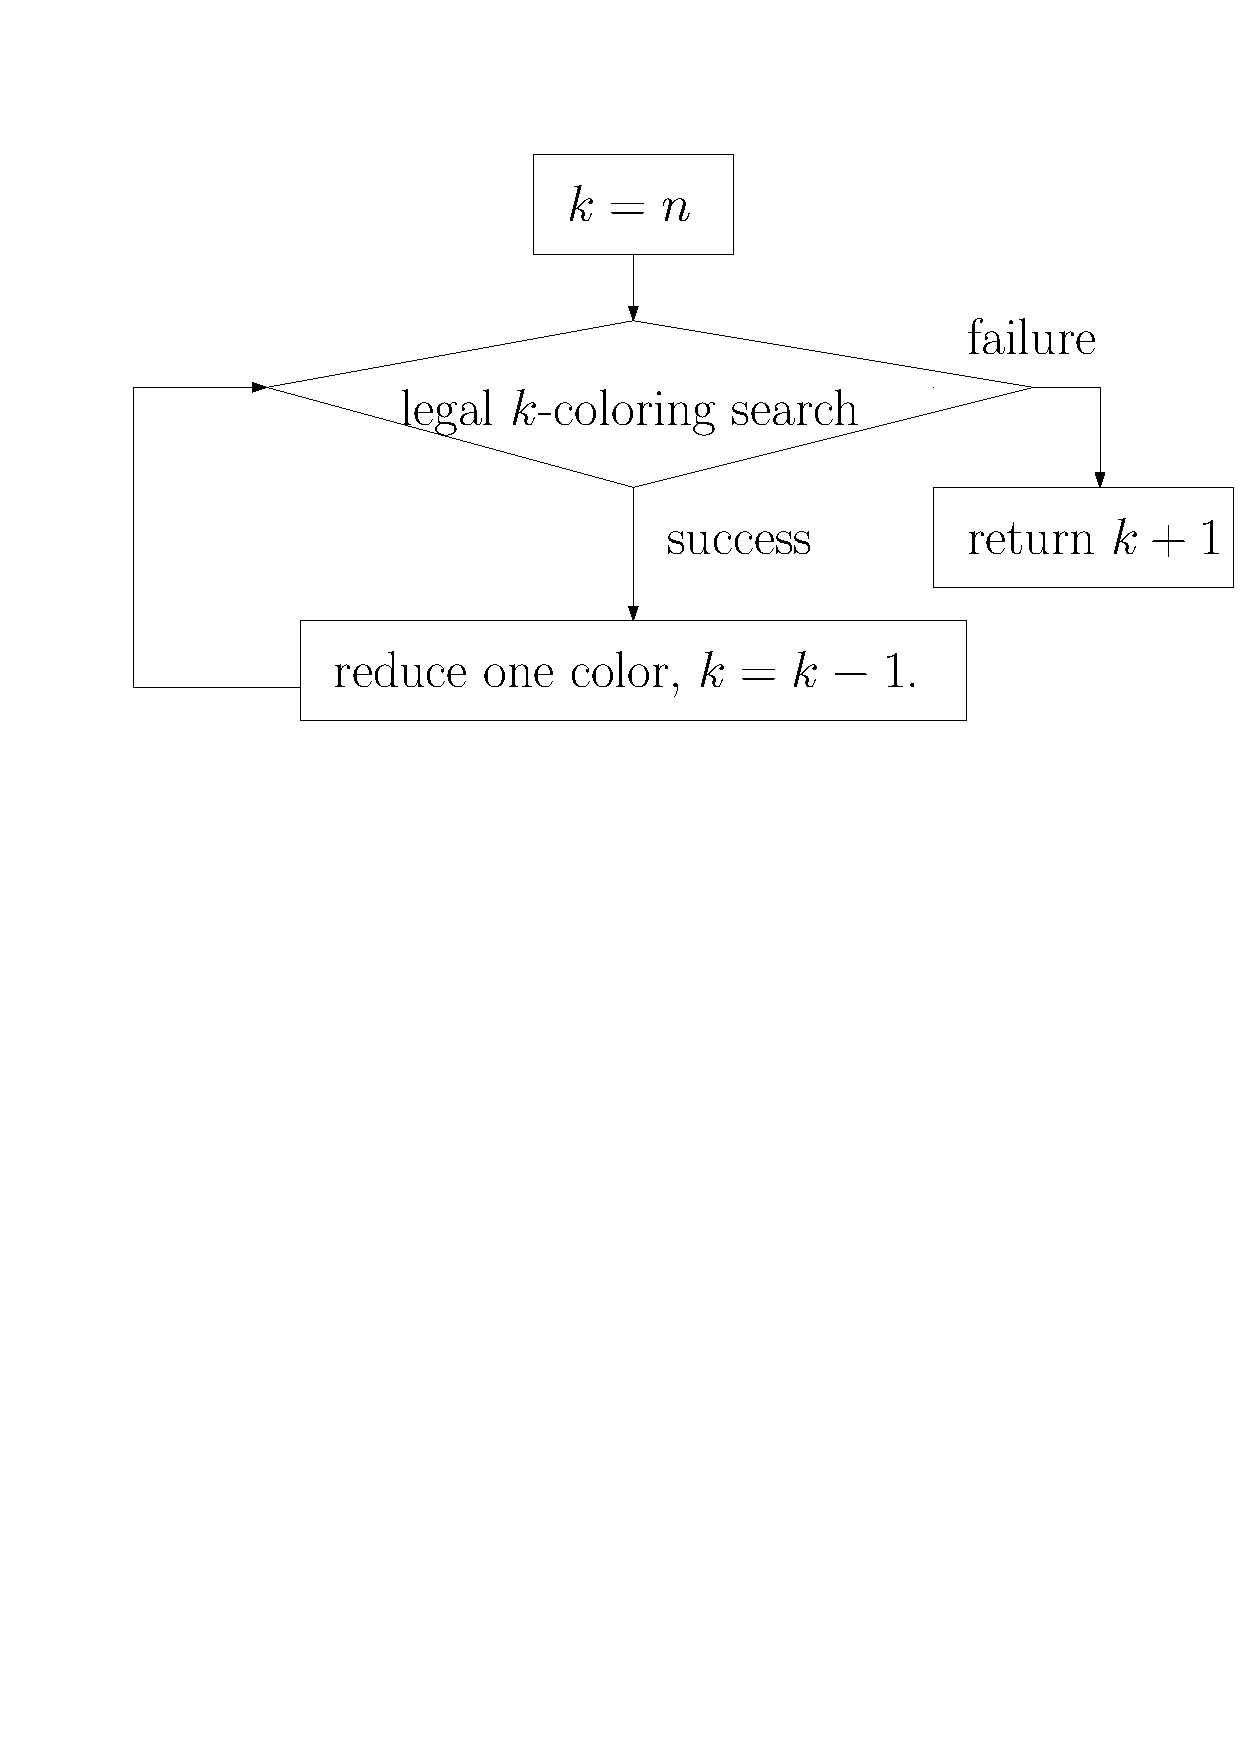
\includegraphics[scale = 0.5]{1/gcpSolver.pdf}
  \caption{GCP-solver}
  \end{figure}
\emph{\textbf{Step 1: Build an initial coloring}}\\
\label{Step 1: Build an Initial Coloring}
A legal $n$-coloring is obviously available. In our GCP-solver, the initial coloring is $c$: $v_i\rightarrow i$. A possible alternative is to build the initial coloring randomly. In Experiment 1 in section 5 (see ~\ref{sec:Experiment 1}) we compare these two alternatives. Our suggestion shows some advantages in performance.\\ 

\emph{\textbf{Step 2: Solve k-GCP using Tabucol}}\\

 
\emph{\textbf{Step 3: Reduce one color}}\\
A $(k-1)$-coloring will be built by reducing the least used color in the previous $k$-coloring. If some color is chosen for reduction, all the nodes in this color will be colored with other remaining colors randomly. If only a few nodes are involved in the color reduction, the resulted $(k-1)$-coloring is more likely to be legal or illegal with few conflicting edges.  

In next section, the data structure of our GCP-solver is introduced.
\clearpage
\subsection{Data structures}
\label{subsec:Data structures}
\emph{\textbf{Tabu Map and Tabu Queue}}\\
 In the process of tabu search, all the legal candidates should be considered in the order of decreasing conflict numbers. To avoid using the forbidden candidates in the search process, a data structure should provide whether a candidate is a tabu or not. The forbidden moves are stored in a map, called \emph{Tabu Map}. Here a one-step move [v, i] is represented by an ordered pair $(v, i) $.\\
After its duration of tabu status, a  forbidden move will be freed. In the meantime, a one-step move will be marked as a tabu move after one search step. Accordingly, a queue called \emph{Tabu Queue} will be used to update the forbidden moves stored in the \emph{Tabu Map}. The size of the \emph{Tabu Queue} is $L+ f(n)\times \alpha$.\footnote{The size of the \emph{Tabu Queue} is adapted to the conflict number.}
When the color of a vertex $v$ is changed, $(v,c(v))$ is recorded in the  \emph{Tabu Map} and also enqueued in the \emph{Tabu Queue}. When the \emph{Tabu Queue} is full, extra forbidden moves  will be popped from the other end of the \emph{Tabu Queue} and will be deleted in the \emph{Tabu Map}, which means the moves are freed.\\

When the color of a vertex $v$ is changed: \\
1. Record $(v, c(v))$ in the \emph{Tabu Map}.\\
2. Insert $(v, c(v))$ in the back of the \emph{Tabu Queue}.\\
3. If the queue is full (size of queue > $L+ f(n) \times\alpha$), we remove the oldest pair $(u,i)$.\\
4. Delete $(u, i)$ in \emph{Tabu Map}. go to step 3\\

An alternative data structure is using an $n \times k $ Matrix T                      \cite{galinier2006survey}. $T_{ij}$ stores the index of iteration, in which the one-step move $[v_i, j]$ is marked as a tabu move. To determine whether a one-step move $[v, i]$ is a tabu move or not, $T_{ij}$ is checked in constant time. If $T_{ij}\geq $ \emph{currentIter} - L - $\alpha \times f(n)$, this move is permitted \footnote{CurrentIter is the index of the current iteration.}. Otherwise, the move is a tabu move.\\

\emph{\textbf{Solution Matrix}}\\
Local search is a search where only small changes are made in each search step. In our situation, only one node is involved in getting to a neighbor of the current coloring. The most time in Tabucol is spent for finding the best one-step move in the complete neighborhood. To reuse the calculated results, Galinier uses a matrix to record the information about the neighborhood \cite {galinier2006survey}. It is the most important data structure in our implementation. This matrix is denoted as \emph{Solution Matrix} $M.$ The matrix $M$  evaluates the candidate moves of the current $k$-coloring $c$. If $c(v_j) = i$, $M_{ij}$ is the number of conflicting edges incident to $v_j$ in the current solution. $\frac{\sum_{j=1}^n M_{c(v_j)j}}{2}$ is the conflict number of solution $c$;
If $c(v_j)\neq i$, $M_{ij}$ is the number of conflicts involving $v_j$ in a neighbor coloring $c'$ of $c$:

$c'(v_j) = i$.\\
 $c'(v_q) = c(v_q), q \neq i,q \in \{1..n\}.$ \\
 
$\Gamma(j,i)=M_{c(v_{j})j}-M_{ij}$ evaluates the improvement of the move $[v_j, i]$ in constant time. To find the best one-step move, all neighbors must be evaluated by the evaluation function $\Gamma$. To find the best one-step move, $O (k\times n)$ time will be spent scanning the \emph{Solution Matrix}.
This matrix is filled at the beginning based on the initial solution and constantly changed. If the chosen one-step move is $[v_i, j]$, which means changing the color of $v_i$ from current color $c(v_i)$ to $j$, some entities in matrix $M$ must be updated. More precisely, for each incident vertex $v_w$ of $v_i$, $M_{c(v_i) w}$ will be decreased by one and  $M_{j w}$ will be increased by one.
\begin{table}[h!]
\begin{minipage}{\textwidth}                                                                                         
\begin{center}
    \begin{tabular}{| l | l |p{6cm}|}
\hline 
    Data Structure & Relevant Operations & Functions \\ \hline
    
    
   \emph{Tabu Map} &\pbox{20cm}{\hspace{1cm}
   \\insert an element\\  erase an element\\search for an element\\}& store and update tabu moves\\ \hline
            
   
    \emph{Tabu Queue}&\pbox{20cm}{\hspace{1cm}\\enqueue an element\\dequeue en element\\}&free tabu moves after a duration\\ \hline
   \pbox{20cm}{\hspace{1cm}\\ \emph{Solution Matrix C}\\ \hspace{1cm}} &\pbox{20cm}{\hspace{1cm}\\change values of few entities constantly\\ \hspace{1cm}}& record information of neighbors\\ \hline
\end{tabular}
\caption[data structure]{Overview of used data structure}
\end{center}
\end{minipage}
\end{table}

Here is a pseudo code of our GCP-solver with the data structures introduced above:


\begin{algorithm}[h!]\label{Original solver}
\SetKwInOut{Input}{input}
\SetKwInOut{Output}{output}
\SetKwInOut{Parameter}{parameter}
 \Input{A Graph in DIMACS standard format}
 \Parameter{L, $\alpha$}
 \Output{the minimum size $k$, a $k$-coloring $c$}
 Build the initial coloring $c$ with $c(v_i) = i$ and the corresponding \emph{Solution Matrix} $M$;\;
 $k = n$;\;
 \While{$(k>1)$}{
    $c'$ = reduceOneColor($c$);\;
	\eIf{$($Tabucol$(c')$ succeed $($See Algorithm \ref{Tabucol with data structures}$))$}{
		$c=c'$;\;
		$k=k-1$;\;
	}{return $k$, $c$}
 }
 \caption{original GCP-solver with data structures}
 \end{algorithm}
\begin{algorithm}[h!]\label{Tabucol with data structures}
 \While{$(f(c') =\sum\nolimits_{i=1}^n {M_{c'(v_i), i}} \neq 0$ $\land$ Timeout does not occur$)$}{
\emph{max} = $-n$;\;
  \For{$(j<k,)$}{
     \For{$(i<n \land j \neq c'(i))$}{
		\If{$((i, j)$ not in Tabu Map $\land$ $  M_{c'(i), i}-M_{ji} > max)$}{
			\emph{max} = $M_{c'(i),i}-M_{ji}$; \;
			(\emph{changedColor}, \emph{changedVertex})  = $(j,i)$;\;
            }   
     }  
  }
    \emph{oldColor} = $c'$(\emph{changedVertex});\;
  $c'$(\emph{changedVertex}) = \emph{changedColor}; \; 
  \For{$(i \in \{1..n\})$}{
  \If{$($ $v_i$ is incident to changedVertex$)$}{
  	 $M_{\emph{oldcolor}, {v_i}} = M_{\emph{oldcolor}, {v_i}}-1$;\;
   	 $M_{\emph{changedColor}, {v_i}} = M_{\emph{changedColor}, {v_i}}+1$;\;
 }
 }
  insert (\emph{oldColor}, \emph{changedVertex}) in \emph{Tabu Map};\;
  push (\emph{oldColor}, \emph{changedVertex}) in \emph{Tabu Queue};\;
  \While{$($\emph{size(}Tabu Queue$)$ > $L + \alpha \times f(c')$ $)$}{
	\emph{Tabu Queue} pops a move (u,v);\;
	delete (u,v) in \emph{Tabu Map}; \;
  }
 }
  \eIf{$(f(c') = 0)$}{return ``success''}{return  ``failure'' }
 \caption{Tabucol with data structures}
 \end{algorithm}
\subsection{Improvement through randomly generated solution}
\label{subsec:Improvement through randomly generated solution}
Generally, finding a $(k+1)$-coloring is easier than finding a $k$-coloring. In first iterations of our GCP-solver, a legal $k$-coloring can be quickly generated by reducing the least used color in the $(k+1)$-coloring to other remaining colors. The Tabucol searches take more time gradually and the most time spent in the process is in finding a legal $c$-coloring and trying to find a $(c-1)$-coloring, where $c$ is the optimal solution. The idea here comes from the observation of time spent in Tabucol searches. It seems that the solution loses its potential in the process of reducing colors iteratively. So it should be helpful to use a new and perhaps more potential coloring. In our GCP-solver, we replace the current illegal solution  occasionally by a new randomly generated coloring of the same size. This randomly generated coloring will be used for the further search.

Experiment 2 (see \ref{sec:Experiment 2}) describes the details of this suggestion and evaluates its performance. It shows Improvement in $53\%$ of our benchmarks.
\subsection{Improvement through changing solution matrix traverse direction}
\label{subsec:traverse}
When searching for the best move in our implementation, the maximum element in the conflict matrix must be found. In the pseudo code above (see Algorithm \ref{Tabucol with data structures}), the matrix is  traversed row by row. If more than one candidate with maximum improvement exists, the first one is chosen as the next step. This matrix can also be traversed column by column. Through Experiment 3 (see \ref{sec:Experiment 3}), we found a GCP-solver with traversal by column usually gets a better result.  
\iffalse
\begin{figure}[h!]
\centering
  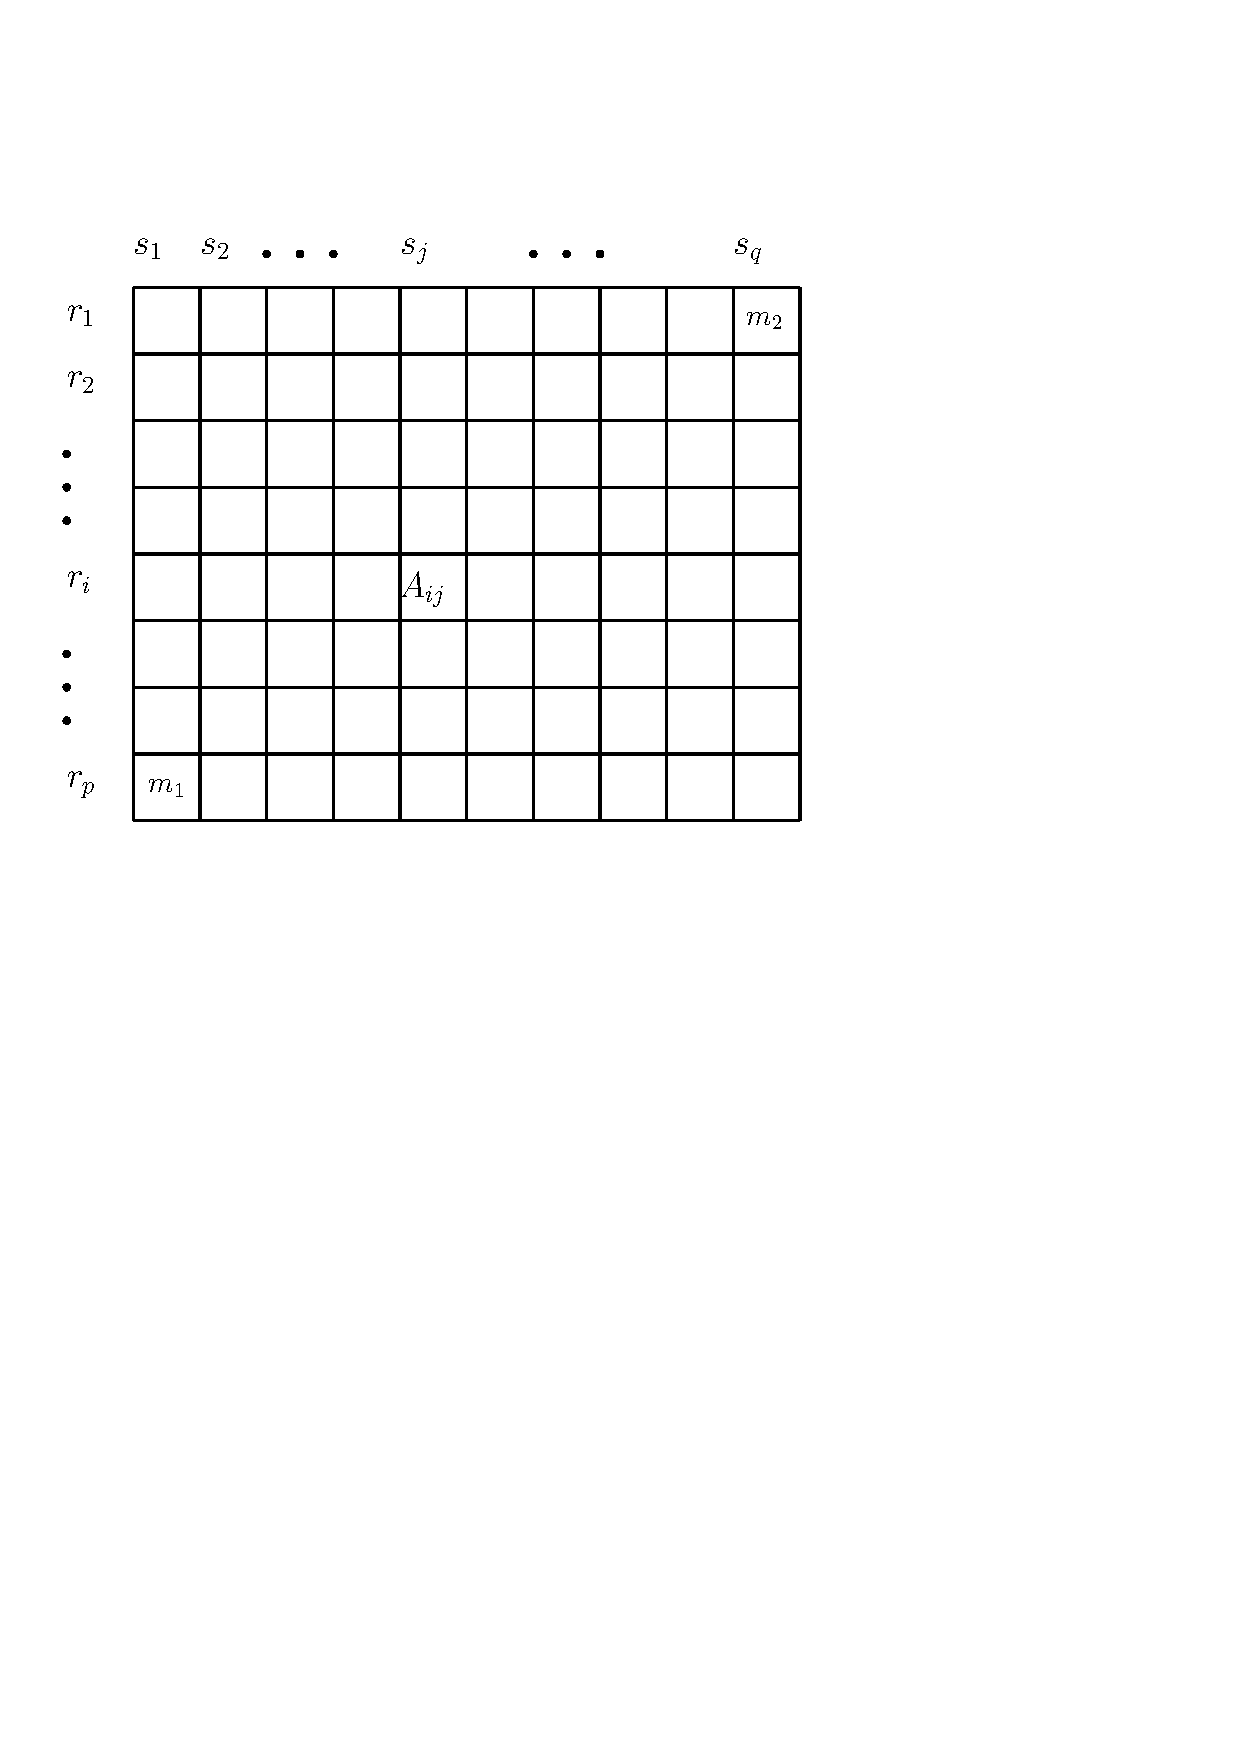
\includegraphics[scale = 0.5]{1/matrixC.pdf}
  \caption{Two candidates $m_1$ and $m_2$ exist in two ends in the minor diagonal of the solution matrix.}
  \label{fig:maC}
  \end{figure}
A simple explanation of this benefit is in the situation where there exist always two best candidate in two ends in minor diagonal in the conflict matrix (see Figure \ref{fig:maC}). The horizontal traversal will find $m_1$ first and set it as best move. In vertical traversal, otherwise, the $m_2$ will found first. If this situation exist for several rounds, if travel in one direction, that means, the algorithm prefer the candidate in one end of the minor diagonal. The bottom left candidates are to change colors of vertices with small indexes. The Traversal in one direction prefers changes of first nodes rather than others. This tendency will lead to some bad performance.
The top right candidates corresponds to using first colors to change the color in solution. This will lead to a concentration of colors, which may be beneficial to the future reduction of colors.
In experiment 3 ref{sec:Experiment 3}, we compare two traverse directions. The result shows a benefit of using column traverse.
\fi
\subsection{Improvement through statistic matrix}
\label{subsec:statistic}
The Tabucol algorithm uses a tabu list to avoid short-term cycling. When the cycling is long (longer than the size of tabu queue), the loop of one-step moves will not be recognized in the search process. An Improvement in our implement is to use a matrix, called \emph{statistic matrix S}. The $S_{ij}$ represents how many times a one-step move $[v_i,j]$ was chosen as the next step. When the search is stuck in one long-term loop, the involved entities in the statistic matrix are increased constantly. If more than one candidate with the highest improvements exists, the candidate with the smallest statistic value will be chosen in the next step. We can also use the entity $S_{ij}$ to determine the possibility of choosing the next move randomly (see Experiment 4 in      \ref{sec:Experiment 4}). \\
\clearpage
\section{Our Parallel Algorithm}
\label{sec:Our parallel Algorithm}
With different kinds of cooperative search, this section presents 4 parallel local search algorithms. The algorithm is based on our GCP algorithm introduced in section 3 and the agents cooperate by sharing different kinds of information. The Performances were compared by experiments in section 5.

\subsection{1st Approach: The pure portfolio approach}
The local search in section \ref{sec:Solving GCP by Tabucol} uses Tabucol as a subroutine to solve the graph coloring problem. The result of the algorithm is a legal coloring of the graph of minimum size. In the algorithms, some parameters like $L$, $\alpha$, the search directions (see section  \ref{subsec:traverse}) and whether a statistic matrix is introduced (see section \ref{subsec:statistic}) affect the one-step moves chosen by the search. The performance of the algorithm is different with different parameter combinations. In the pure portfolio version of our algorithm, the agents run the GCP solver with different parameter combinations. After collecting the solutions found by each agent, the search takes the coloring of the minimum size as the result.
This approach improved the performance compared to the parallel GCP solver, in which all agents run with the same parameters (see experiment 5). For each graph, there is one parameter combination that is most suitable in the  aspect of the size of tabu list and the search path of this combination is better than others. So trying different parameter combinations will improve the performance.

\subsection{2nd Approach: Forced color reducing}
This approach is based on the pure portfolio approach with different parameter combinations as shown above. 
This approach  is called GCP-solver with forced color reducing (FCR). As its name suggests, the agents share the minimum size found by all agents. Because of different parameter combinations, some agents are ``luckier'' and decrease the size of coloring more quickly. Suppose that one agent has already found a $k$-coloring, where the other agents still make an effort to determine whether the graph is $(k+i)$-colorable (integer $i > 0$). In this approach, the lucky agent will broadcast this message. With this notification, all agents confirm that the graph is at least a $k$-colorable graph. Then the agents in the process of searching for a $(k + i)$ ($i \geq 0$) coloring will abandon the current search and search for a legal $(k-1)$ coloring since a legal $k$-coloring is already found. This approach saves a lot of  effort and makes the search space larger with different implementation in our experiment (see experiment 6 in section \ref{sec:Experiment 6}), the strategy we use is to reduce the least used $(i+1)$ colors in the current $(k + i)$ coloring. This generated $(k - 1)$ coloring is used as the initial coloring in the Tabucol search for a legal $(k - 1)$ coloring. In this paper, this strategy is called  forced color reducing (FCR).
\subsection{3rd Approach: Tabu sharing}
\label{subsec: tabu sharing}
One character of tabu search is using a tabu list to record the search path to avoid short-term cycling. In previous parallel approaches, each agent manages and uses one tabu list of its own.
The idea behind this approach is to share the ``traps'' of local search loops. So sharing the tabu list should be able  to bring an improvement in the cooperation of agents. This approach is called parallel GCP-solver with tabu sharing.
We did an experiment to test the performance of this approach (see experiment 7 in section \ref{sec:Experiment 7}). It shows, however, a worse performance compared to the original parallel GCP-solver.
According to our observation in the implementation, we list 3 possible reasons:\\
1. Not all tabu moves are traps. Some critical moves which are necessary to get the optimal result are only explored by a part of threads while other threads threat them as tabu moves. The threads missing these critical steps would never contribute to the algorithm.\\
2. Best candidates are forbidden. In hard graphs, it is normal to have several best candidate moves in the current solution. Some candidates involve different parts in the graph. The solution will be optimized to the greatest extent by going over the candidate moves and the order of the moves have no effect on the optimization. Figure \ref{Figure tabushare} is an example with two best candidates.  The current coloring $c$ has two best candidate moves $m_1$, $m_2$. The candidate  $m_1$ is ($v_1$, white). The $m_2$ is ($v_2$, black). The optimal coloring of the example graph will be reached by making the move $m_1$ then $m_2$ or inversely. Imagine that we have two agents  $a_1$ and  $a_2$ work with the same coloring $c$. The agent $a_1$ inspects $m_1$ and pushes $m_1$ in shared tabu list. After that, the agent $a_2$ makes the move $m_2$ and marks $m_2$ as a tabu move. In this deadlock case, the agent $a_1$ cannot take $m_2$ even it brings the best improvement on the current solution. Similarly, agent $a_2$ recognize $m_1$ as a tabu move and does a compromise with other suboptimal moves.
\begin{figure}[h]
\centering
  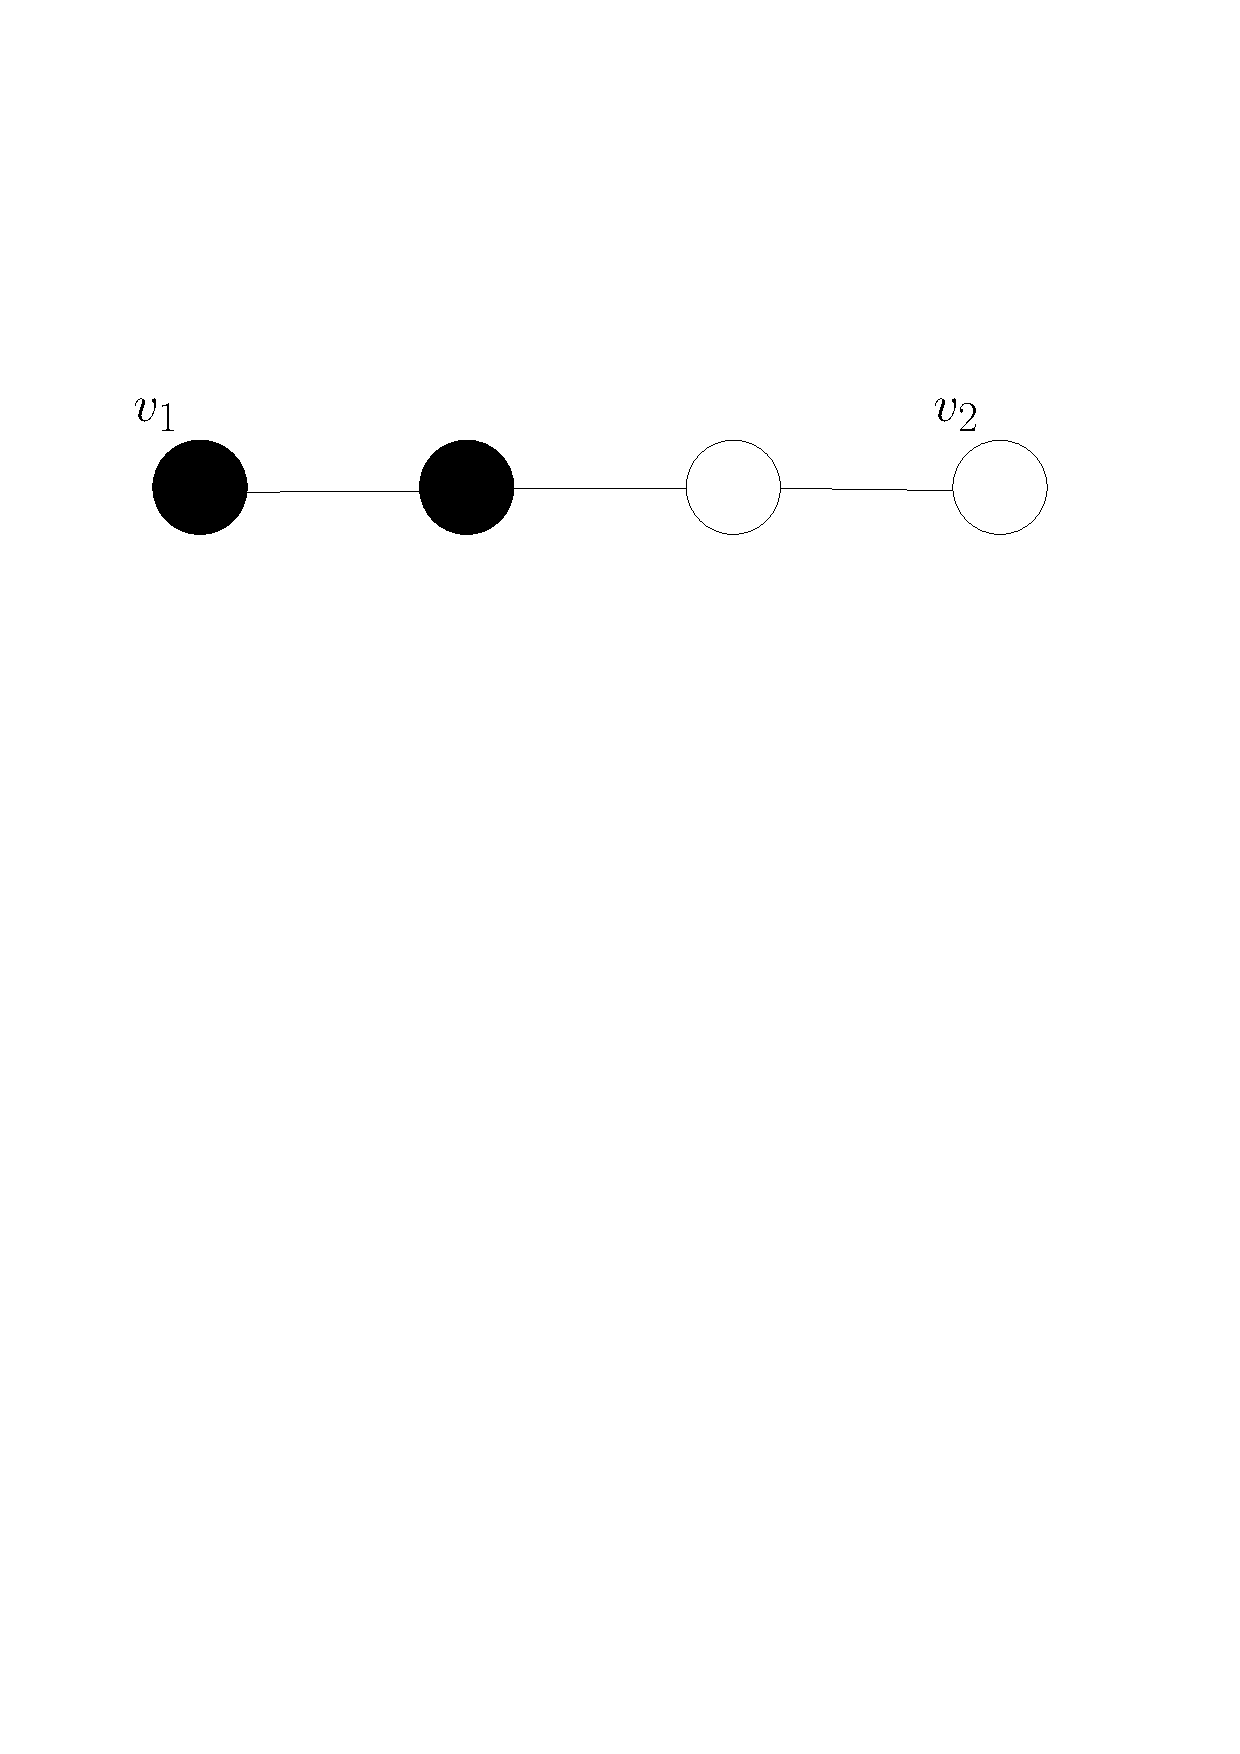
\includegraphics[scale = 0.8]{images/1/tabushare.pdf}
      \caption{ An example with two moves $m_1$ and $m_2$. The candidate  $m_1$ is ($v_1$, white). The $m_2$ is ($v_2$, black).}
      \label{Figure tabushare}
\end{figure}

3. When a move is taken earlier by one agent, it will be ignored by other agents. The differences in parameters make the colorings of agents more different and thus the shared tabu moves may not be meaningful to other agents. In some cases, the tabus from other agents disturb the choice of next moves.
\subsection{4th Approach: Statistic sharing}
\label{4th Approach: Statistic sharing}
After the analysis of the failures in the 3rd Approach with tabu sharing, we came up with the approach with statistic matrix sharing. The intention of this sharing is to use the statistic matrix to recognize the real traps and warn other agents when one agent is stuck in one loop.
The Tabucol search in agents follows the scheme below:\\
1. The agents use one common statistic matrix. The statistic matrix counts the times of moves chosen by one agent.\\
2. When two best candidates exist in one solution, the move with smaller statistic matrix value will be chosen.\\
3. When only one best candidate exists with a very large statistic value, the search will choose another candidate randomly.\\
This approach demonstrates a big improvement. (see Experiment 8)
\clearpage
\section{Evaluation}
The single-threaded experiments were run on computers that had four AMD(R) Opteron(R) processors 6168 (1.9 Ghz with 12 cores) and 256GB RAM. The computers ran the 64-bit version of Ubuntu 12.04. The multi-threaded experiments were run on fat nodes InstitutsClusterII (IC2) at Steinbuch Centre for Computing (SCC) of KIT. IC2 is a distributed memory parallel computer with 480 16-way so-called thin compute nodes and 5 32-way so-called fat compute nodes. The thin nodes are equipped with 16 cores, 64 GB main memory, whereas the fat nodes are equipped with 32 cores, 512 GB main memory \cite{ic2}.
\subsection{DIMACS standard format}


All the graphs used in experiments are in the DIMACS standard format                     \cite{johnson1996cliques}. This format is a widely used format to test and compare graph coloring algorithms. A DIMACS file contains the description of an instance using three types of lines\footnote{Only unweighted undirected simple graphs are tested in our experiments. For other descriptors and details of the DIMACS format, see \cite{dimacs}.}:\\
\\
1. Comment line: Comment lines give information about the graph for human readers, like the author of the file or related works. A comment line starts with a lower-case character $c$ and will be ignored by programs:\\
\centerline{\textbf{c} \emph{\# this is an example of the comment line \#}}\\
\\
2. Problem line: The problem line appears exactly once in each DIMACS format file. The problem line is signified by a lower-case character $p$. For a graph $G=(V,$ $E)$, the problem line in its DIMACS file is:\\
\centerline{\textbf{p} edge |V| |E|}\\
\\
3. Edge Descriptor: An edge $\{u, v\}$ in the graph is described in an edge Descriptor:\\
\centerline{\textbf{e} u v}\\


\begin{figure}[h!]
\begin{center}
  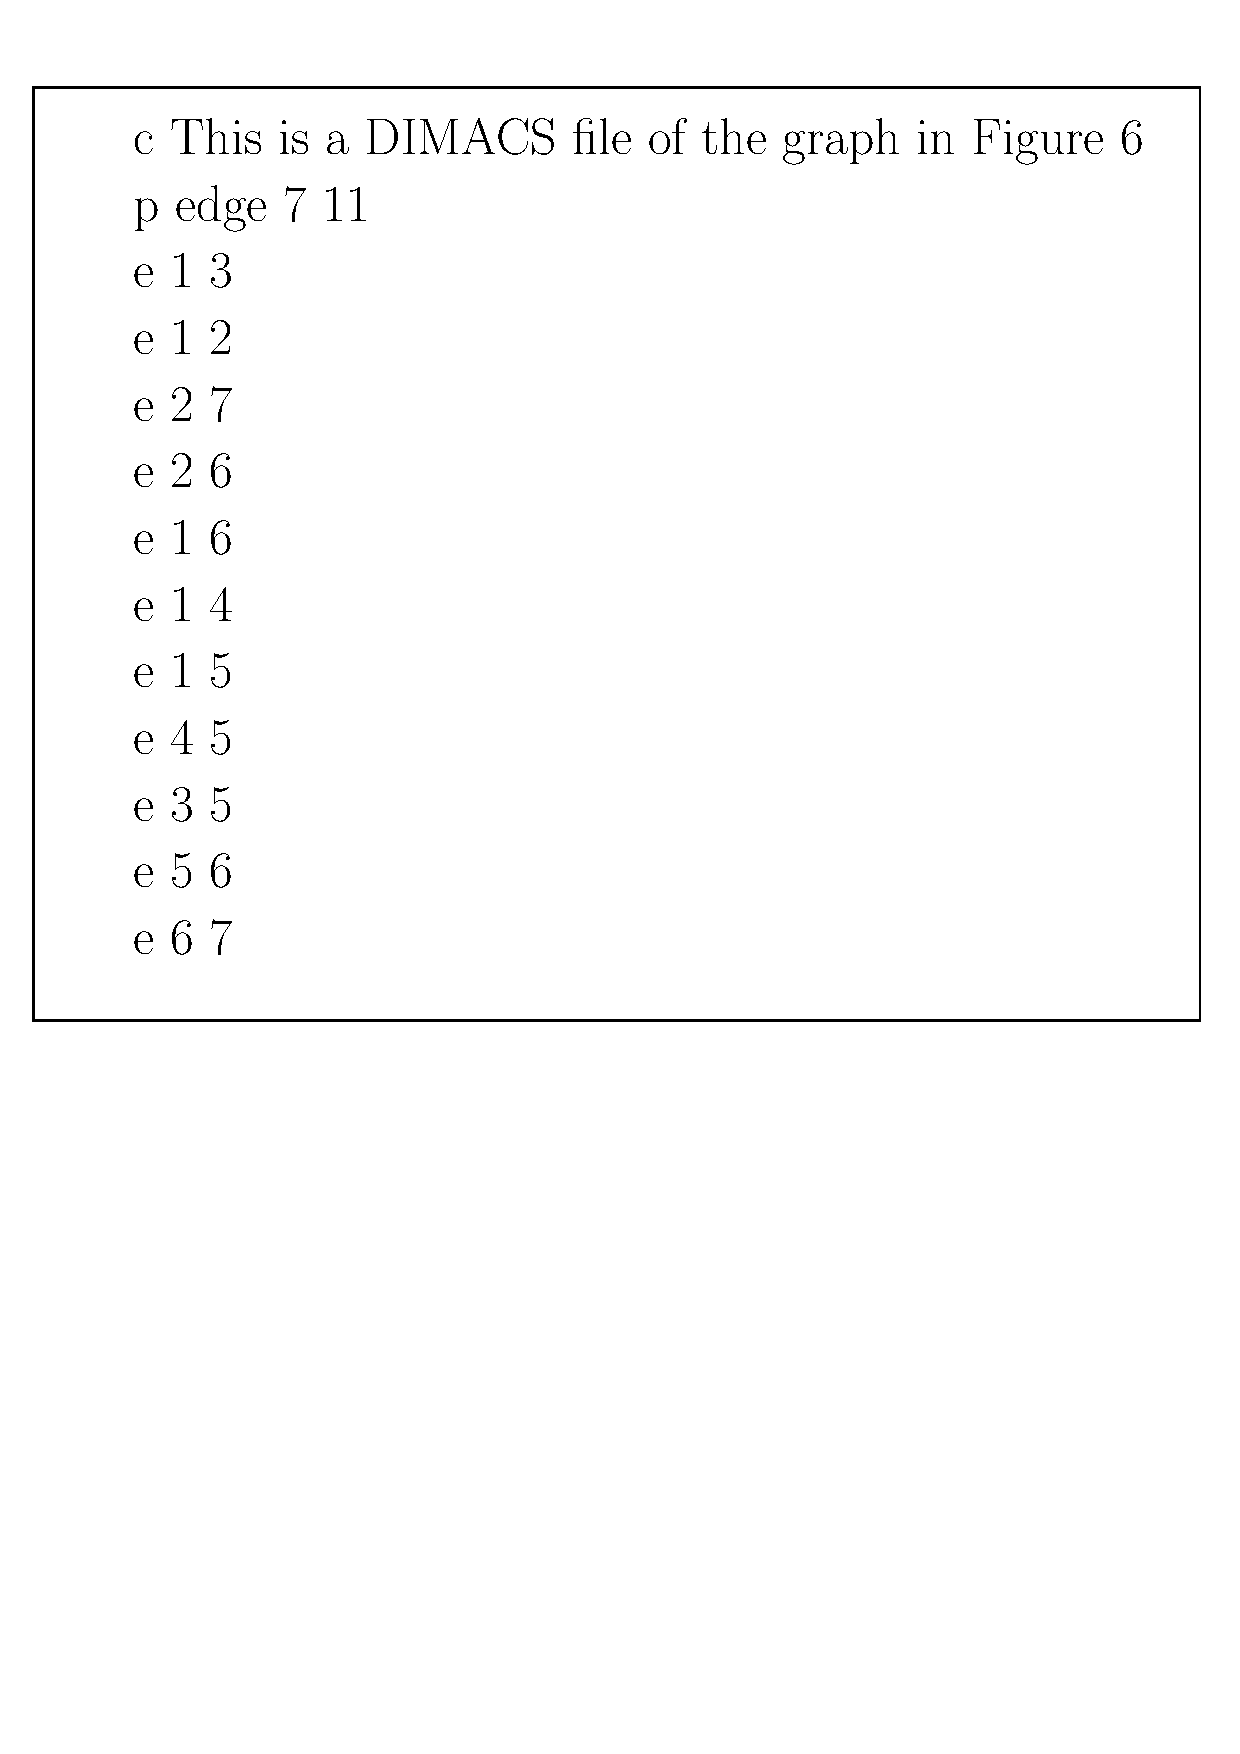
\includegraphics[scale = 0.5]{1/Dimacs.pdf}
      \caption{A DIMACS file example of the graph in Figure \ref{Figure 6}}
      \end{center}
\end{figure}


\subsection{Benchmarks}
\label{benchmark}
The graphs used in our experiments are from the DIMACS benchmark collection    \cite {graph1, graph2}. In the following experiments, 68 graphs are used. Some names of the graphs contain generation involved information:\\

 \textbf{dsjcX.Y and dsjrX.Y}: Graphs generated by Johnson et.al \cite{johnson1991optimization}. $X$ in the file name denotes the number of vertices. The probability that two nodes are incident is given by $Y.$\\
\textbf{flatX\_K}: Graphs generated by J Culberson. The graphs are generated by partitioning its vertices in $K$ nearly same sized sets and adding edges which connect vertices in different sets. So the chromatic number is theoretically smaller or equal to $K$.\\ 
 \textbf{le450\_K}: Graphs with 450 vertices and chromatic number $K$ \cite{leighton1979graph}.\\
 \textbf{c*}: Huge graphs with more than 4 million edges.\\
 \textbf{latin\_square\_10 and school*}: A latin square graph (and class scheduling graphs respectivelly) generated by Gary Lewandowski for the second Dimacs challenge.\\
 \textbf{r*.X}: Random graphs. The suffix ``c'' denotes the complement of a graph.\\
 \textbf{queenX\_Y}: Graphs translated from Stanford GraphBase with ID: gunion(board(X,Y,0,0,-1,0,0),board(X,Y,0,0,-2,0,0),0,0).\\
 \textbf{milesX}: Graphs translated from Stanford GraphBase with ID:miles(128,0,0,0,X,127,0).\\
 \textbf{jean}: Graphs translated from Stanford GraphBase with ID: book(jean,80,0,1,356,0,0,0).\\
 \textbf{fpsol2.i.*, inithx.i.*, mulsol.i.*, zeroin.i.*}: Graph generated from a register problem based on real code.\\
\textbf{brockX\_*}: Graphs with $X$ nodes generated by Mark Brockington and Joe Culberson. 
 
 
 In our experiments, the graphs are divided into 4 classes according to their size and complexity for the graph coloring problem \footnote{In the experiments, the performance of the algorithms after a time interval was compared.}. For huge graphs in the first class, the timeout is set to 20 minutes. For the second class, the timeout is 4 minutes. For the third class 2 minutes and for fourth class 1 minute.\\
 
\textbf{class 1} (4 graphs): c2000.5, r1000.5, dsjc1000.9, c4000.5.\\

\textbf{class 2} (3 graphs): dsjc1000.5, r1000.1c, latin\_square\_10.

\textbf{class 3} (53 graphs):\\ miles250, jean, queen8\_8, le450\_5a, le450\_5b, queen9\_9, le450\_5c, le450\_5b, queen8\_12, queen10\_10, queen11\_11, queen12\_12, queen13\_13, queen14\_14, queen15\_15, le450\_15b, miles500, queen16\_16, le450\_15c, le450\_25a, le450\_25b, le450\_15d, dsjc1000.1, school1,\\ school1\_nsh, zeroin.i.2, zeroin.i.3, fpsol2.i.3, fpsol2.i.2, inithx.i.2, inithx.i.3, miles750, mulsol.i.2, mulsol.i.3, mulsol.i.4, mulsol.i.5, miles1000, mulsol.i.1, zeroin.i.1, inithx.i.1, dsjc500.5, fpsol2.i.1, miles1500, brock400\_1, brock400\_2, brock400\_3, dsjr500.1c, flat1000\_60\_0,\\ flat1000\_50\_0, flat1000\_76\_0, brock800\_1, brock800\_2, brock800\_4, dsjr500.5.col.\\

\textbf{class 4} (7 graphs): dsjc500.1, le450\_25c, le450\_25d, dsjc250.5, flat300\_28\_0, r250.5, dsjc500.9. 
 \subsection{Used plots and tables}
Different plots and tables are used to illustrate the results of the following experiments.\\

\emph{\textbf{Comparison Table}}\\
See Table \ref{tab:com} for example.\\
A comparison table shows the different results of algorithms. The first column contains the names of graphs. The fields of a comparison table in the following columns corresponds to the coloring sizes found with an algorithm.

\emph{\textbf{Scatter Plot}}\\
See Figure \ref{Experiment 1 scatter plot} for an example.\\
A scatter plot compares the results of two algorithms. Similar to the comparison table, only the graphs with a difference in two algorithms are shown in the scatter plot.  The x-axis shows the color sizes for an algorithm, denoted by x-axis algorithm. The vertical axis to the left shows the color sizes for  y-axis algorithm. A graph with color size $u$ in x-axis algorithm and color size $v$ in y-axis algorithm corresponds to a mark $(u, v)$. The line $x = y$ divides the plot into two parts. The marks in the upper part $(x < y)$ correspond to graphs with better results for the x-axis algorithm. The opposite corresponds to better results for the y-axis algorithm. 
 In Figure \ref{Experiment 1 scatter plot}, the part above the diagonal line contains more marks than the lower part, which means x-axis algorithm is better than the y-axis algorithm.\\
 
\emph{\textbf{Cactus Plot}}\\
See Figure \ref{Experiment 1 cactus plot} for an example.\\
In a cactus plot, the problems are indexed in an ascending order of color size. The y-axis shows the result sizes of the graph. Each algorithm corresponds to a curve in different colors. The point $(u, v)$ on a curve means a $v$-coloring is found in the corresponding algorithm for the $u$th graph.\\
\emph{\textbf{Advantage Plot}}\\
See Figure \ref{Experiment 1 advantage plot} for an example.\\
An Advantage plot shows the advantage of algorithms to an comparison algorithm. The y-axis gives the ordered percentage difference. A relative difference  upper the line $x = 0$ corresponds to an advantage of the algorithm in the corresponding graph. The opposite is true for an advantage of the comparison algorithm.



 \subsection{Automatic parameter optimization}
The parameter combinations used in the experiments are generated with the help of the algorithm parameter optimization tool SMAC \cite{SMAC} (sequential model-based algorithm configuration). SMAC ran our algorithms on our instances (class 4 as training instances, class 1 as test instances.) using different parameter combinations and seeds. In this simulation process, the performance of different combinations was evaluated. With the help of SMAC, $32$ optimal parameter combinations were found. The $32$ parameter combinations used in our experiments are as follows:\\

\begin{center}
\captionof{table}{parameter combinations}
\label{table:parameter combinations}
  \begin{tabular}{| l | l l l l l l |p{2cm}|}
   \hline
Index&L& $\alpha$ &Initialization&Replace&Traverse& Statistic\\ \hline
1&9 &0.38 &Node-Index&true&Column&true\\
2&1 &0.77&Node-Index&true&Column&true\\
3&11 &0.90&Node-Index&true&Column&true \\
4&17 &0.59&Random&true&Column&true \\
5&18 &0.42&Node-Index&false&Column&false\\\hline
6&4 &0.92&Node-Index&true&Column&true \\
7&16 &0.76&Node-Index&false&Row&false\\
8&17 &0.47&Node-Index&false&Column&false\\
9&2 &0.60&Node-Index&true&Column&false\\
10&2 &0.54&Node-Index&false&Column&true\\\hline
11&5 &0.46&Random&true&Column&true\\
12&11 &0.63&Random&true &Column&true\\
13&7 &0.83&Node-Index&true&Column&true\\
14&8 &0.98&Node-Index&false &Row&true\\
15&18 &0.58&Node-Index&true&Column&false \\\hline
16&13 &0.90&Node-Index&false&Column&true \\
17&20 &0.56&Node-Index&true &Column&false\\
18&10&0.95&Node-Index&true &Column&true\\
19&15 &0.55&Node-Index&true&Row&true\\
20&17 &0.39&Node-Index&true&Column&true \\\hline
21&18 &0.52&Node-Index&false&Column&true\\
22&11 &0.32&Node-Index&true&Column&true \\
23&15 &0.62&Node-Index&false&Column&true \\
24&6 &0.94&Random&true&Column&true\\
25&9 &0.94&Node-Index&false&Column &false\\\hline
26&12 &0.96&Node-Index&true&Column&true\\
27&16 &0.58&Node-Index&false&Column&true\\
28&9 &0.45&Node-Index&false&Column&true\\
29&19 &0.95&Node-Index&true&Column&true \\
30&18 &0.31&Node-Index&true&Column &false\\\hline
31&6 &0.50&Node-Index&false&Column&false\\
32&15 &0.93&Node-Index&false&Column &false\\\hline


    \end{tabular}
\end{center}
For a single thread algorithm, we use the first parameter combination. In a multi-threaded algorithm, the $i$th thread uses the $i$th parameter combination. The parameter L and $\alpha$ determine the size of the tabu List with  $L+ f(n)\times \alpha$. For the initial solution generation, two choices exist: randomly generated initialization and node-index initialization (see section \ref{Step 1: Build an Initial Coloring}). The solution matrix is traversed row by row or column by column (see section \ref{subsec:traverse}). The combinations with ``statistic = true'' use the statistic matrix while searching and participating statistic sharing (see section \ref{4th Approach: Statistic sharing}).
\clearpage
\subsection{Experiments}
In experiment 1 to experiment 4, we compare strategies of the single-thread GCP-solver shown in section \ref{sec:Solving GCP by Tabucol}. The results are in table \ref{tab:com}. The original solver is an implementation of algorithm \ref{Original solver} with the data structures shown in section \ref{subsec:Data structures}. Experiment 1 compares this original Solver, which uses a randomly generated initial solution with a GCP-solver with the strategy ``Node-Index initialization'' (see section \ref{Step 1: Build an Initial Coloring}). Experiment 2 compares our original solver with the solver with the strategy ``replacement'' (see section \ref{subsec:Improvement through randomly generated solution}). Experiment 3 compares the original solver, which traverses the solution matrix row by row with a solver with the column traversal (see section \ref{subsec:traverse}). Experiment 4 proves the advantage of adding the data structure statistic matrix (see section \ref{subsec:statistic}). The results of these experiments are summarized in table \ref{tab:com}.\\
Experiments 5 to 8 are about the parallel GCP solver. The experiments perform with 1 core, 2 cores, 4 cores, 8 cores, 16 cores and 32 cores. The experiments use our single-thread GCP solver with Node-index initialization and the 3 advantageous strategies we found (see sections \ref{subsec:Improvement through randomly generated solution}, \ref{subsec:traverse},  \ref{subsec:statistic}) for comparisons. Experiment 5 compares this single-thread GCP solver with multi-threaded solver with different parameter combinations, denoted as the pure portfolio GCP-solver. Experiments 6 to 8 compare our pure portfolio GCP-solver with the parallel solver with cooperation. Experiment 6 tests the performance of the parallel solver with minimum color size sharing among agents. Experiment 7 shows the solver with shared tabu list, which turns out to be a failed attempt. In experiment 8, the parallel solver with shared statistic matrix is compared with the pure portfolio solver. \\
In experiment 9, we compare our parallel GCP-solver with all found advantageous coopeartion with three DSATUR-based algorithms (see section \ref{comparison}).
\clearpage
\subsubsection{Experiment 1: Random initialization vs Node-index initialization}
\label{sec:Experiment 1}
Experiment 1 compares two different strategies of initialization in our GCP-solver. Our suggestion is to use c: $v_i \rightarrow i$ as the initial solution. 
Another alternative is to build a coloring randomly. In table \ref{tab:com}, the column ``Original solver'' uses the random initialization. The column ``NodeIndex'' contains the results with the Node-index initialization. In 29 of the 68 graphs, there is a performance difference between two initializations. 24 graphs get a better result with our version. 5 graphs get a better result with a random initial solution.
\begin{figure}[h!]
\begin{center}
  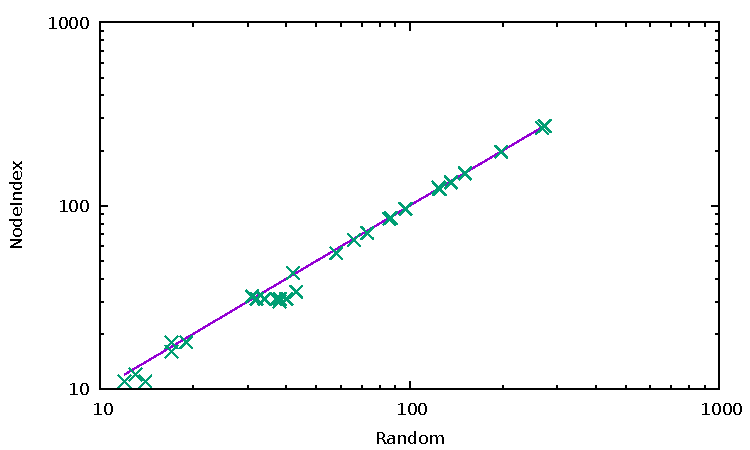
\includegraphics[scale = 1]{Experiments/E1/scalog.pdf}
  \end{center}
  \caption{Two suggestions have very similar performance since all points are close to the diagonal. The fact that most points are over the diagonal shows that our suggestion has marginal advantages over random initialization. Every graph in Table \ref{tab:com} with different results  is plotted as a green cross.}
  \label{Experiment 1 scatter plot}
  \end{figure}
  
 \begin{figure}[h!]
\centering
  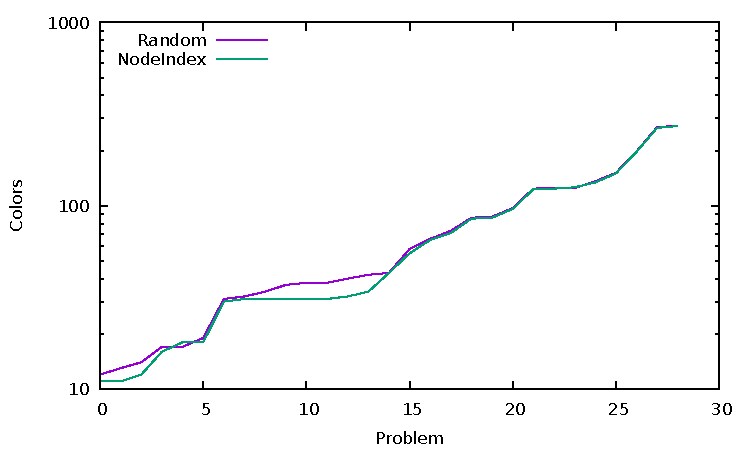
\includegraphics[scale = 1]{Experiments/E1/caclog.pdf}
    \caption{Our suggestion shows advantages especially for small graphs.}
      \label{Experiment 1 cactus plot}
  \end{figure}
\begin{figure}[h!]
\centering
  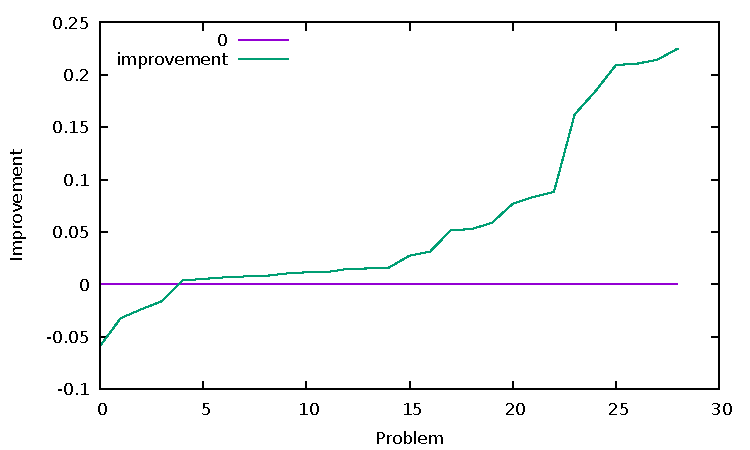
\includegraphics[scale = 1]{Experiments/E1/impro.pdf}
      \caption{advantage plot NodeIndex: Random}
      \label{Experiment 1 advantage plot}
\end{figure}

\subsubsection{Experiment 2: Original solver vs Solution replacement}
\label{sec:Experiment 2} 
The GCP-solver introduced in section \ref{sec:Solving GCP by Tabucol} runs within a time interval \emph{t}. In our suggestion, the current coloring will be replaced by a randomly generated coloring of the same size when a Tabucol search fails after $\lfloor t/2 \rfloor$. 

Comparing the original GCP-solver and our suggestion which replaces the current illegal solution after half of the time interval, our suggestion shows improvement in 36 graphs. The results are shown in Table \ref{tab:com} (column ``Replacement''). 

\begin{figure}[h!]
\centering
  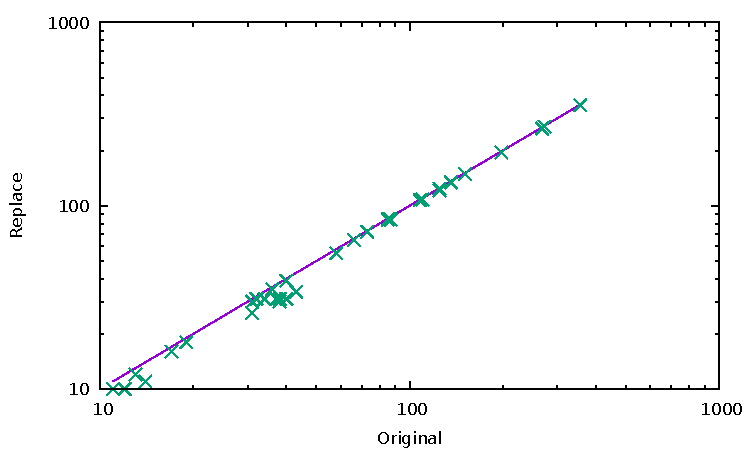
\includegraphics[scale = 1]{Experiments/E2/scalog.pdf}
  \caption{The points below the diagonal show an advantage of our suggestion.}
  \end{figure}
\begin{figure}[H]
\centering
  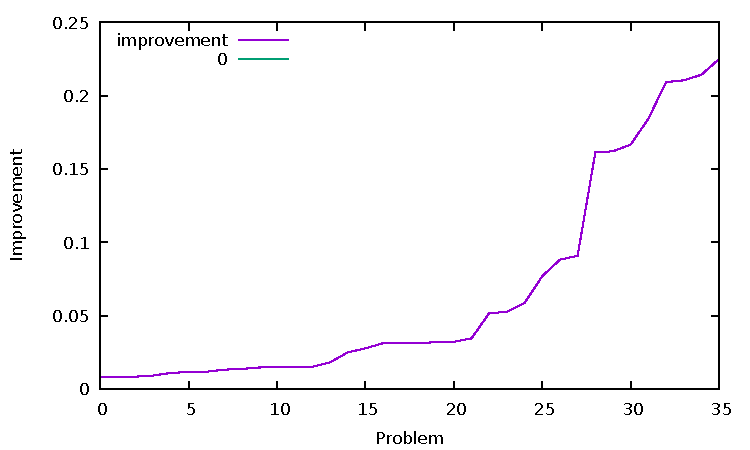
\includegraphics[scale = 1]{Experiments/E2/impro.pdf}
      \caption{The improvement of our suggestion is very small
       (most relative differences are under 0.1\%). However, this suggestion is adopted because of its universal improvement (more than 53\% graphs are improved with our suggestion).}
\end{figure}

\subsubsection{Experiment 3: RowTraverse vs ColumnTraverse}
\label{sec:Experiment 3}
In our Implementation, we use the conflict matrix to evaluate the one step moves. The suggestion \emph{RowTraverse} traverses the matrix row by row to find the best candidate. If more than one best candidates exist, it will always choose the first one for the next move. Our suggestion called \emph{ColumnTraverse} traverses the conflict matrix column by column and uses the first best candidate for the next move. In experiment 3, the \emph{ColumnTraverse} shows advantages in more than half of the graph instances (see table \ref{tab:com} column ``Ctraverse'').
\begin{figure}[h!]
\centering
  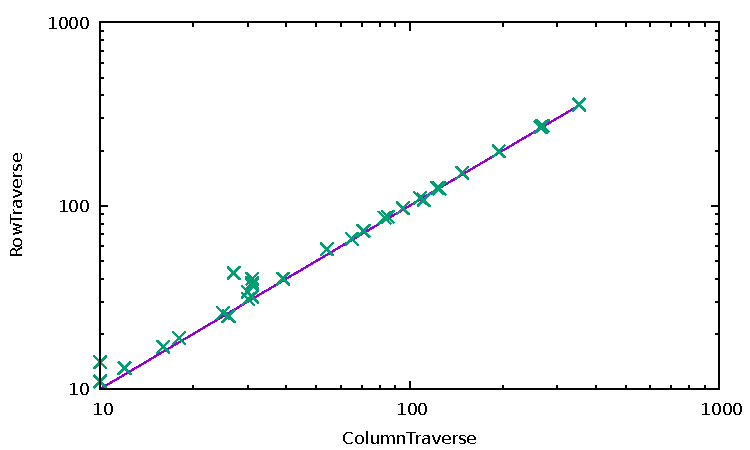
\includegraphics[scale = 1]{Experiments/E3/scalog.pdf}
      \caption{The scatter plot compares the \emph{RowTraverse} and \emph{ColumnTraverse}. The advantage of \emph{ColumnTraverse} concentrates on small graphs. For large graphs, two traverse directions get similar results.}
\end{figure}

\begin{figure}[h!]
\centering
  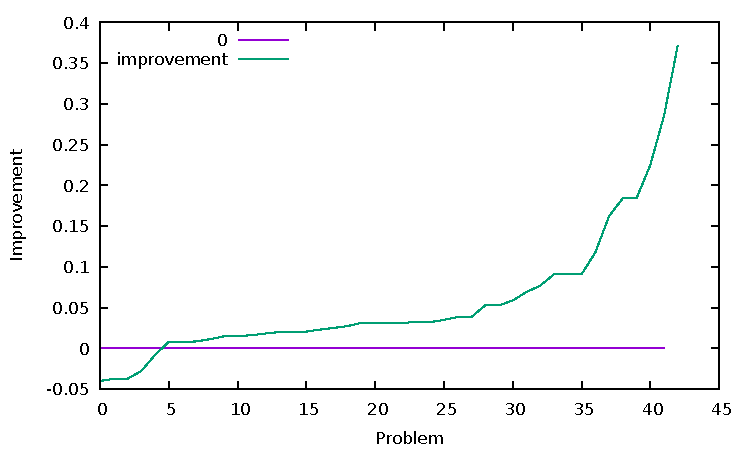
\includegraphics[scale = 1]{Experiments/E3/impro.pdf}
      \caption{ 43 graphs of our instances get small differences by \emph{RowTraverse}  and \emph{ColumnTraverse}. 38 graphs get better results with  \emph{ColumnTraverse} and 5 graphs benefit from \emph{RowTraverse}.}
\end{figure}

\subsubsection{Experiment 4: Original solver vs Statistic solver}
\label{sec:Experiment 4}
In our GCP-solver, we add an $n\times n$ statistic matrix to record the repeated steps in the past. The aim of adding this statistic matrix is to avoid long-term cycling of the local search in a neighborhood. When a cycling is longer than the length of the tabu list, the original GCP-solver will be stuck in the cycling, while the solver with statistic matrix can realize this and jump out of this cycling by choosing candidates which are not involved in this cycling.
In Experiment 4, the original GCP-solver is compared with a GCP-solver with statistic matrix $S$. The $S_{ij}$ corresponds to how many times [$v_i$, j] is chosen as the best move. When a move [$v_i$, j] is chosen for the next step in the search, $S_{ij}$ is increased by one. If two best candidates exist, the corresponding entities in the statistic matrix will be compared. The candidate which is less used before will be chosen as the next move. When the value of one entity in statistic matrix reaches a predefined upper bound (In our experiment, the upper bound is $n$), the suboptimal candidate will be used in the next move. The results of this experiment are in table \ref{tab:com} (see column ``Statistic'').



\begin{figure}[h!]
\centering
  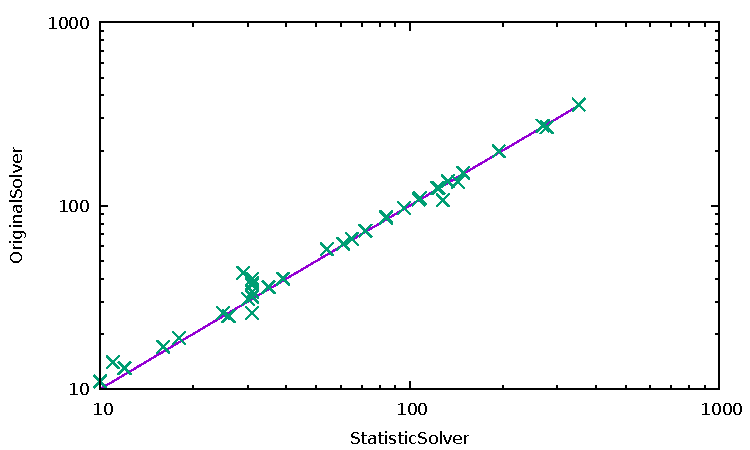
\includegraphics[scale = 1]{Experiments/E4/scalog.pdf}
  \caption{Scatter plot of 44 graphs in our benchmark with differences between the original GCP-solver (OriginalSolver) and the solver with statistic matrix (StatisticSolver)}
  \end{figure}
\begin{figure}[h!]
\centering
  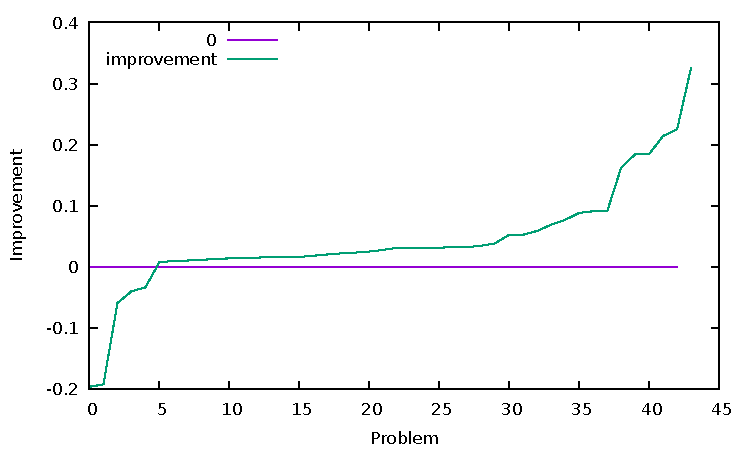
\includegraphics[scale = 1]{Experiments/E4/impro.pdf}
      \caption{39 graphs of 68 graph instances (57\% graphs) get a better result with help of a statistic matrix. 5 graphs (7\% graphs) get a better result without statistic matrix.}
\end{figure} 
\begin{landscape}
\begin{table}[]
\label{tab:com}
\caption{
The original GCP-solver uses a randomly generated initial solution. It traverses the solution matrix row by row. The original solver is implemented with the data structure shown in \ref{subsec:Data structures}, statistic matrix not included.}
\footnotesize
    \begin{tabular}[t]{|p{2.2cm}|p{1.4cm} p{1.4cm}p{1.2cm} p{1.2cm} p{1cm} p{1.2cm}|}
\hline
Graph&Original&Node-Index&Replace&Ctraverse&Statistic&Our solver\\ \hline
miles250&\textbf{8}&\textbf{8}&\textbf{8}&\textbf{8}&\textbf{8}&\textbf{8}\\ 
jean&\textbf{10}&\textbf{10}&\textbf{10}&\textbf{10}&\textbf{10}&\textbf{10}\\
queen8\_8&11&11&\textbf{10}&\textbf{10}&\textbf{10}&\textbf{10}\\
le450\_5a&11&11&11&\textbf{10}&\textbf{10}&\textbf{10}\\ 
le450\_5b&11&11&11&\textbf{10}&11&11\\ \hline
queen9\_9&12&11&\textbf{10}&12&12&11\\ 
le450\_5c&13&\textbf{12}&\textbf{12}&\textbf{12}&\textbf{12}&\textbf{12}\\ 
le450\_5d&14&11&11&\textbf{10}&11&12\\ 
queen8\_12&\textbf{13}&\textbf{13}&\textbf{13}&\textbf{13}&\textbf{13}&\textbf{13}\\
queen10\_10&\textbf{13}&\textbf{13}&\textbf{13}&\textbf{13}&\textbf{13}&\textbf{13}\\ \hline
queen11\_11&\textbf{14}&\textbf{14}&\textbf{14}&\textbf{14}&\textbf{14}&\textbf{14}\\
queen12\_12&\textbf{15}&\textbf{15}&\textbf{15}&\textbf{15}&\textbf{15}&\textbf{15}\\
queen13\_13&\textbf{16}&\textbf{16}&\textbf{16}&\textbf{16}&\textbf{16}&\textbf{16}\\ 
dsjc500.1&17&\textbf{16}&\textbf{16}&\textbf{16}&\textbf{16}&\textbf{16}\\
queen14\_14&\textbf{17}&18&\textbf{17}&\textbf{17}&\textbf{17}&\textbf{17}\\ \hline
queen15\_15&19&\textbf{18}&\textbf{18}&\textbf{18}&\textbf{18}&\textbf{18}\\ 
le450\_15b&19&19&19&\textbf{18}&\textbf{18}&\textbf{18}\\
miles500&\textbf{20}&\textbf{20}&\textbf{20}&\textbf{20}&\textbf{20}&\textbf{20}\\
queen16\_16&\textbf{20}&\textbf{20}&\textbf{20}&\textbf{20}&\textbf{20}&\textbf{20}\\ 
le450\_15c&26&26&26&\textbf{25}&\textbf{25}&\textbf{25}\\ \hline
le450\_25a&26&26&26&\textbf{25}&26&\textbf{25}\\
le450\_25b&\textbf{25}&\textbf{25}&\textbf{25}&26&26&\textbf{25}\\
le450\_15d&31&32&\textbf{26}&31&31&\textbf{26}\\ 
dsjc1000.1&\textbf{26}&\textbf{26}&\textbf{26}&\textbf{26}&31&\textbf{26}\\
school1&43&34&34&\textbf{27}&29&33\\ \hline
school1\_nsh&34&31&31&30&31&\textbf{29}\\ 
zeroin.i.2&31&31&\textbf{30}&\textbf{30}&\textbf{30}&\textbf{30}\\ 
zeroin.i.3&31&31&31&\textbf{30}&\textbf{30}&\textbf{30}\\ 
fpsol2.i.3&38&\textbf{30}&\textbf{30}&31&31&\textbf{30}\\
fpsol2.i.2&37&31&31&31&31&\textbf{30}\\ \hline
inithx.i.2&40&\textbf{31}&\textbf{31}&\textbf{31}&\textbf{31}&\textbf{31}\\ 
inithx.i.3&38&\textbf{31}&\textbf{31}&\textbf{31}&\textbf{31}&\textbf{31}\\
le450\_25c&32&32&\textbf{31}&\textbf{31}&\textbf{31}&\textbf{31}\\ 
le450\_25d&32&32&32&\textbf{31}&\textbf{31}&\textbf{31}\\\hline 
\end{tabular}
\begin{tabular}[t]{|p{2.2cm}|p{1.4cm} p{1.4cm}p{1.2cm} p{1.2cm} p{1cm} p{1.2cm}|}
\hline
Graph&Original&Node-Index&Replace&Ctraverse&Statistic&Our solver\\ \hline
miles750&32&32&\textbf{31}&\textbf{31}&\textbf{31}&\textbf{31}\\
mulsol.i.2&\textbf{31}&\textbf{31}&\textbf{31}&\textbf{31}&\textbf{31}&\textbf{31}\\
mulsol.i.3&32&\textbf{31}&\textbf{31}&\textbf{31}&\textbf{31}&\textbf{31}\\
mulsol.i.4&\textbf{31}&\textbf{31}&\textbf{31}&\textbf{31}&\textbf{31}&\textbf{31}\\
mulsol.i.5&\textbf{31}&\textbf{31}&\textbf{31}&\textbf{31}&\textbf{31}&\textbf{31}\\ \hline
dsjc250.5&36&36&\textbf{35}&36&\textbf{35}&\textbf{35}\\
flat300\_28\_0&40&40&\textbf{39}&\textbf{39}&\textbf{39}&\textbf{39}\\ 
miles1000&\textbf{42}&43&\textbf{42}&\textbf{42}&\textbf{42}&\textbf{42}\\ 
mulsol.i.1&\textbf{49}&\textbf{49}&\textbf{49}&\textbf{49}&\textbf{49}&\textbf{49}\\ 
zeroin.i.1&\textbf{49}&\textbf{49}&\textbf{49}&\textbf{49}&\textbf{49}&\textbf{49}\\  \hline
inithx.i.1&58&55&55&\textbf{54}&\textbf{54}&\textbf{54}\\
dsjc500.5&62&62&62&62&\textbf{61}&\textbf{61}\\
fpsol2.i.1&66&\textbf{65}&\textbf{65}&\textbf{65}&\textbf{65}&\textbf{65}\\ 
r250.5&73&\textbf{71}&72&\textbf{71}&72&\textbf{71}\\
miles1500&\textbf{73}&\textbf{73}&\textbf{73}&\textbf{73}&\textbf{73}&\textbf{73}\\ \hline
brock400\_1&86&85&85&\textbf{83}&84&84\\ 
brock400\_2&87&86&\textbf{84}&85&\textbf{84}&\textbf{84}\\ 
brock400\_3&85&85&\textbf{84}&85&85&\textbf{84}\\ 
dsjr500.1c&97&96&97&\textbf{95}&96&96\\
flat1000\_60\_0&108&108&107&111&107&\textbf{106}\\ \hline
flat1000\_50\_0&107&107&107&111&107&\textbf{106}\\ 
flat1000\_76\_0&\textbf{107}&\textbf{107}&\textbf{107}&111&128&\textbf{107}\\ 
dsjc1000.5&110&110&\textbf{108}&\textbf{108}&\textbf{108}&\textbf{108}\\ 
r1000.1c&125&123&\textbf{121}&123&123&123\\ 
brock800\_1&125&124&124&124&\textbf{123}&\textbf{123}\\ \hline 
brock800\_2&125&125&\textbf{124}&\textbf{124}&\textbf{124}&\textbf{124}\\
brock800\_4&\textbf{124}&126&\textbf{124}&125&\textbf{124}&\textbf{124}\\ 
latin\_square\_10&136&134&134&136&\textbf{133}&\textbf{133}\\
dsjr500.5&135&135&135&135&143&\textbf{134}\\ 
dsjc500.9&151&150&149&\textbf{148}&149&149\\\hline 
c2000.5&198&197&195&\textbf{194}&\textbf{194}&\textbf{194}\\ 
r1000.5&268&266&264&265&277&\textbf{263}\\ 
dsjc1000.9&273&272&270&\textbf{269}&\textbf{269}&\textbf{269}\\ 
c4000.5&356&356&353&353&\textbf{352}&\textbf{352}\\ \hline
\end{tabular}
\end{table}
\end{landscape}

\clearpage
\subsubsection{Experiment 5: Original solver vs Parallel solver with various parameter combinations}
Our parallel implementation uses OpenMP to support shared memory multiprocessing. Our pure portfolio approach takes advantage of flexible parameter combinations. The slave threads execute the GCP-solver with different parameter combinations in parallel. Then the result of each agent is written in a shared memory. The master thread compares the results and chooses the result with minimum size as the final result.

\begin{algorithm}[H]
\SetKwInOut{Input}{input}
\SetKwInOut{Output}{output}
\SetKwInOut{Parameter}{parameter}
 \Input{A Graph in DIMACS standard format, number of agents $t$}
 \Parameter{parameter combinations $\{p_1, p_2,..., p_t\}$}
 \Output{Solution $s$}
start $t$ agents;\;
Each agent runs GCP-solver with parameter combination $p_{index\_of \_t}$;\;
solutions $\{s_1, s_2,...,s_t\}$ found by agents are collected and compared;\;
Output the coloring of the minimum size from $\{s_1, s_2,..., s_t\}$;\;
 \caption{parallel GCP-solver with different parameter combinations}
 \end{algorithm}
In experiment 5, we compare our pure portfolio GCP-solver with a single-threaded GCP-solver. The parallel GCP-solver with $t$ threads use the first $t$ parameter combinations in table \ref{table:parameter combinations}.
\begin{figure}[h!]
\centering
  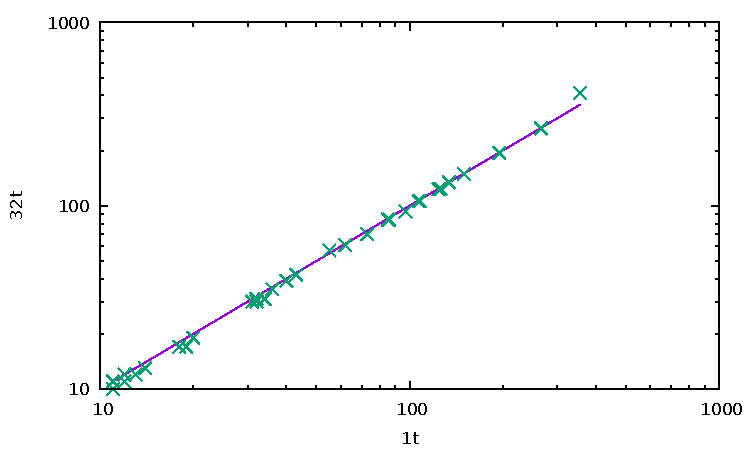
\includegraphics[scale = 1]{Experiments/E5/scalog.pdf}
      \caption{The scatter plot compares our single-threaded GCP-solver and the pure portfolio solver with 32 threads. Most points are under the diagonal. One outlier (the huge graph c4000.5) is on the right top, which seems to be caused by the time spent on swapping to hard disk when RAM is full.}
\end{figure} 
\begin{table}[H]
\begin{center}
    \begin{tabular}{| l |l| l | l|l|l|p{1cm}|}
\hline
&1t&2t&4t&8t&16t&32t\\ \hline
best& 0&8&9&23&29&34\\ \hline
unique&0&0&2&0&1&9\\ \hline
    \end{tabular}
\captionof{table}{For a pure portfolio approach, the numbers of times of getting the minimum size among all the solvers are recorded in the row ``best''. The row ``unique'' records the times of getting the unique minimum size. This table is based on the 40 graphs shown in table \ref{table:basic parallel GCP-solver}.}
\end{center}
\end{table}
\begin{table}[H]
\begin{center}

    \begin{tabular}{| l | l l l l l p{1cm}|}
\hline
Graph&1t&2t&4t&8t&16t&32t\\ \hline
queen8\_8&11&11&11&\textbf{10}&\textbf{10}&\textbf{10}  \\ 
le450\_5a&11&11&11&\textbf{10}&\textbf{10}&\textbf{10}  \\
le450\_5b&11&11&11&\textbf{10}&\textbf{10}&\textbf{10}  \\
queen9\_9&11&11&\textbf{10}&11&11&11  \\
le450\_5c&12&\textbf{11}&\textbf{11}&\textbf{11}&\textbf{11}&12  \\\hline 
le450\_5d&12&\textbf{11}&\textbf{11}&\textbf{11}&\textbf{11}&\textbf{11}  \\ 
queen8\_12&13&13&13&13&\textbf{12}&\textbf{12}  \\
queen10\_10&13&13&13&13&\textbf{12}&\textbf{12}  \\ 
queen11\_11&14&14&14&14&14&\textbf{13}  \\
queen14\_14&18&\textbf{17}&\textbf{17}&\textbf{17}&\textbf{17}&\textbf{17}  \\\hline 
le450\_15b&19&19&19&18&\textbf{17}&\textbf{17}  \\ 
queen16\_16&20&20&20&20&\textbf{19}&\textbf{19}  \\
le450\_15c&26&26&26&26&26&\textbf{25}  \\
school1&34&34&34&\textbf{31}&\textbf{31}&\textbf{31}  \\
school1\_nsh&31&31&31&31&31&\textbf{30}  \\ \hline
zeroin.i.2&31&31&31&\textbf{30}&\textbf{30}&\textbf{30}  \\
le450\_25c&32&32&31&31&31&\textbf{30}  \\ 
le450\_25d&32&32&32&\textbf{31}&\textbf{31}&\textbf{31}  \\ 
miles750&32&32&32&\textbf{31}&\textbf{31}&\textbf{31}  \\ 
dsjc250.5&36&36&36&\textbf{35}&\textbf{35}&\textbf{35}  \\ \hline
flat300\_28\_0&40&\textbf{39}&\textbf{39}&\textbf{39}&\textbf{39}&\textbf{39}  \\
miles1000&43&\textbf{42}&\textbf{42}&\textbf{42}&\textbf{42}&\textbf{42}  \\
inithx.i.1&55&\textbf{54}&55&\textbf{54}&\textbf{54}&57  \\ 
dsjc500.5&62&\textbf{61}&\textbf{61}&\textbf{61}&\textbf{61}&\textbf{61}  \\
r250.5&73&73&71&71&71&\textbf{70}  \\ \hline
brock400\_1&85&85&85&\textbf{84}&\textbf{84}&\textbf{84}  \\
brock400\_2&86&85&85&85&85&\textbf{84}  \\ 
brock400\_3&85&85&85&\textbf{84}&\textbf{84}&\textbf{84}  \\ 
dsjr500.1c&97&97&96&\textbf{93}&\textbf{93}&\textbf{93}  \\ 
flat1000\_60\_0&108&107&107&\textbf{106}&\textbf{106}&\textbf{106}  \\ \hline
flat1000\_50\_0&107&107&107&107&\textbf{106}&\textbf{106}  \\ 
r1000.1c&124&124&124&124&122&\textbf{123}  \\ 
brock800\_1&124&124&124&124&124&\textbf{123}  \\
brock800\_2&125&125&125&\textbf{124}&\textbf{124}&\textbf{124}  \\
brock800\_4&126&\textbf{124}&125&\textbf{124}&\textbf{124}&\textbf{124}  \\ \hline
latin\_square\_10&134&134&134&\textbf{132}&\textbf{132}&134  \\
dsjc500.9&150&150&150&150&150&\textbf{149}  \\
c2000.5&195&195&195&195&195&\textbf{194}  \\ 
r1000.5&266&266&\textbf{264}&\textbf{264}&\textbf{264}&\textbf{264}  \\ 
c4000.5&356&357&\textbf{355}&363&412&412  \\ \hline
    \end{tabular}
\label{table:basic parallel GCP-solver}
\captionof{table}{40 graphs get different results when GCP-solver uses different numbers of threads. The column $n$t ($n\in \{1,2,4,8,16,32\}$) is for the corresponding results of the pure portfolio GCP-solver with $n$ threads. The GCP-solver with one thread is identical to the original GCP-solver introduced in section \ref{sec:Solving GCP by Tabucol}. The graphs in the table are ordered with color size found in the original GCP-solver. }
\end{center}
\end{table}
\subsubsection{Experiment 6: GCP-solver with FRC}
\label{sec:Experiment 6}
In experiment 6 the approach forced color reducing (FRC) was tested.
There is a global variable $k_{min}$ shared by all agents. It represents the minimum size of the legal coloring found by the agents.
The GCP-solver$\_$FCR runs Tabucol iteratively on several agents with different parameter combinations. In the process, the minimum size is shared among the agents.
\vspace{40px} 
The pseudo code is as follows:

\begin{algorithm}[H]
\SetKwInOut{Input}{input}
\SetKwInOut{Output}{output}
\SetKwInOut{Parameter}{parameter}
 \Input{A Graph G in DIMACS standard format, number of agents $t$}
 \Parameter{parameter combinations $\{p_1, p_2,..., p_t\}$, $Timeout$}
 \Output{Solution $s$}
$k_{min}$ = n;\;
 start t agents;\;
//in $t$ Agents\;
$c = initialColoring(G,k)$;\;
$k = n-1$;\;
\While{(Timeout does not occur) }{
$Tabucol(c, k)$; //search a $k$-coloring based on $c$ and set the new coloring as $c$\;
\If{$(k < k_{min}\land Tabucol(c, k)$ succeed$)$}{
	$k_{min}$ = $k$;\;
	}
	$k= k-1$;\;
	$c = reduceOneColor(c, k)$ //reduce the least used color in the current coloring \;
}
 \caption{A parallel GCP-solver with forced color reducing}
 \end{algorithm} 
 \vspace{20px}
The results of our experiment are shown in table \ref{table:GCP-solverFCR}. 49 graphs get different results when GCP-solver\_FCR uses different numbers of threads. Generally, the result is improved with the increase in the number of threads. For the graph c400.5, the results with 16 threads and 32 threads are unusual. A possible cause is that the swapping to hard disk in this huge graph takes a lot of time.\\

\begin{table}[h!]
    \begin{tabular}{| l |l| l | l|l|l|p{1cm}|}
\hline
&1t&2t&4t&8t&16t&32t\\ \hline
best& 2&8&18&24&32&45\\ \hline
unique&0&0&1&1&2&14\\ \hline
    \end{tabular}
\captionof{table}{As the number of threads increases, the numbers of times of getting the minimum size among all the solvers are increased.  The table left is based on the 49 graphs shown in table \ref{table:GCP-solverFCR}. }
\end{table}
\clearpage
\begin{table}
\begin{center}
    \begin{tabular}{| l | l | l|l|l|l|p{1cm}|}
\hline
Graph&1t&2t&4t&8t&16t&32t\\ \hline
queen8\_8&11&\textbf{10}&\textbf{10}&\textbf{10}&\textbf{10}&\textbf{10}\\ 
le450\_5b&11&\textbf{10}&11&\textbf{10}&\textbf{10}&\textbf{10}\\
queen9\_9&\textbf{11}&12&\textbf{11}&\textbf{11}&\textbf{11}&\textbf{11}\\
le450\_5c&12&12&12&11&11&\textbf{10}\\
le450\_5d&12&12&12&11&11&\textbf{10}\\ \hline
queen8\_12&13&13&13&13&\textbf{12}&\textbf{12}\\
queen10\_10&13&13&13&13&\textbf{12}&\textbf{12}\\ 
queen11\_11&14&14&14&14&14&\textbf{13}\\
queen12\_12&15&15&15&15&15&\textbf{14}\\
dsjc500.1&16&16&16&16&\textbf{15}&\textbf{15}\\ \hline
queen14\_14&18&18&\textbf{17}&\textbf{17}&\textbf{17}&\textbf{17}\\
queen16\_16&20&20&20&\textbf{19}&\textbf{19}&\textbf{19}\\
le450\_15c&26&26&26&\textbf{25}&\textbf{25}&\textbf{25}\\ 
le450\_25a&26&\textbf{25}&\textbf{25}&\textbf{25}&\textbf{25}&\textbf{25}\\
le450\_25b&\textbf{25}&26&\textbf{25}&\textbf{25}&\textbf{25}&\textbf{25}\\ \hline
le450\_15d&26&26&26&\textbf{25}&\textbf{25}&\textbf{25}\\ 
dsjc1000.1&26&26&26&26&\textbf{25}&\textbf{25}\\
school1&34&36&33&34&33&\textbf{31}\\ 
school1\_nsh&31&32&32&31&\textbf{29}&30\\ 
zeroin.i.2&31&31&\textbf{30}&\textbf{30}&\textbf{30}&\textbf{30}\\ \hline
zeroin.i.3&31&31&\textbf{30}&\textbf{30}&\textbf{30}&\textbf{30}\\ 
fpsol2.i.2&31&\textbf{30}&\textbf{30}&\textbf{30}&\textbf{30}&\textbf{30}\\ 
le450\_25c&31&32&31&31&31&\textbf{30}\\
le450\_25d&31&31&31&\textbf{30}&31&31\\ 
miles750&32&32&32&\textbf{31}&\textbf{31}&\textbf{31}\\ \hline
dsjc250.5&36&\textbf{35}&\textbf{35}&\textbf{35}&\textbf{35}&\textbf{35}\\ 
flat300\_28\_0&39&39&40&39&39&\textbf{38}\\
miles1000&43&43&\textbf{42}&\textbf{42}&\textbf{42}&\textbf{42}\\ 
dsjc500.5&62&62&62&\textbf{61}&\textbf{61}&\textbf{61}\\ 
r250.5&73&73&\textbf{71}&\textbf{71}&\textbf{71}&\textbf{71}\\ \hline
brock400\_1&85&85&85&84&84&\textbf{83}\\
brock400\_2&85&85&85&85&\textbf{84}&\textbf{84}\\ 
brock400\_3&86&86&85&\textbf{84}&\textbf{84}&\textbf{84}\\ 
dsjr500.1c&95&\textbf{94}&\textbf{94}&96&95&\textbf{94}\\ 
flat1000\_60\_0&107&107&107&107&107&\textbf{106}\\ \hline
flat1000\_50\_0&107&\textbf{106}&\textbf{106}&\textbf{106}&\textbf{106}&\textbf{106}\\ 
flat1000\_76\_0&109&108&\textbf{107}&\textbf{107}&\textbf{107}&\textbf{107}\\ 
dsjc1000.5&109&110&109&108&109&\textbf{107}\\ 
r1000.1c&126&126&125&123&120&\textbf{119}\\ 
brock800\_1&125&124&124&\textbf{123}&\textbf{123}&\textbf{123}\\ \hline
brock800\_2&125&\textbf{124}&\textbf{124}&\textbf{124}&\textbf{124}&\textbf{124}\\ 
brock800\_4&126&124&124&124&\textbf{123}&\textbf{123}\\ 
latin\_square\_10&136&134&\textbf{132}&133&\textbf{132}&\textbf{132}\\ 
dsjr500.5&136&136&135&135&135&\textbf{134}\\ 
dsjc500.9&152&150&\textbf{149}&\textbf{149}&\textbf{149}&\textbf{149}\\ \hline
c2000.5&195&196&195&195&195&\textbf{194}\\ 
r1000.5&268&267&266&264&\textbf{263}&264\\
dsjc1000.9&271&271&270&270&270&\textbf{268}\\ 
c4000.5&356&362&\textbf{354}&357&386&406\\ \hline
    \end{tabular}
\label{table:GCP-solverFCR}
\captionof{table}{GCP-solver\_FCR}
\end{center}
\end{table}
\clearpage
\begin{figure}[h]
  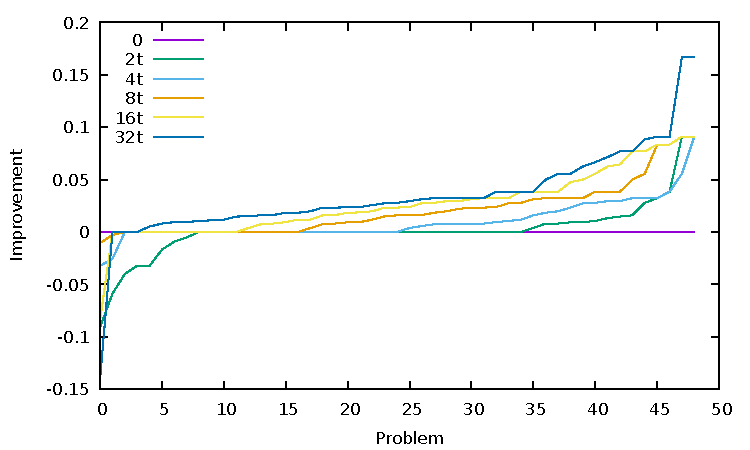
\includegraphics[scale = 1]{Experiments/E6/imp/impro.pdf}
\caption{This advantage plot presents the improvement of GCP-solver through sharing the  global minimum color size among all the agents. The result with 32 threads shows  big and stable improvement.}
\end{figure}
\subsubsection{Experiment 7: GCP-solver with tabu share}
\label{sec:Experiment 7}
Experiment 7 tests the approach of tabu sharing (see \ref{subsec: tabu sharing}). All the agents run the GCP-solver independently and the final result is the minimum size among the agents. The only difference of this approach from the pure portfolio GCP-solver is that all agents share one tabu list, which is built with the parameter combination of the original GCP-solver ($L$ = 9 and $\alpha$ = 0.38). We compare the results of tabu shared GCP-solver with different numbers of threads (see Table \ref{tab:tabu sharing}).
\begin{table}[h!]
\begin{center}
    \begin{tabular}{| l |l| l | l|l|l|p{1cm}|}
\hline
&1t&2t&4t&8t&16t&32t\\ \hline
best& 52&32&18&11&7&5\\ \hline
unique&25&4&0&0&0&0\\ \hline
    \end{tabular}
\captionof{table}{GCP-solver with tabu sharing is a suggestion with bad performance. The more threads share the tabu list, the worse the performance of the search is. The statistical data here are based on table \ref{tab:tabu sharing}.}
\end{center}
\end{table}
\begin{figure}[h!]
\centering
  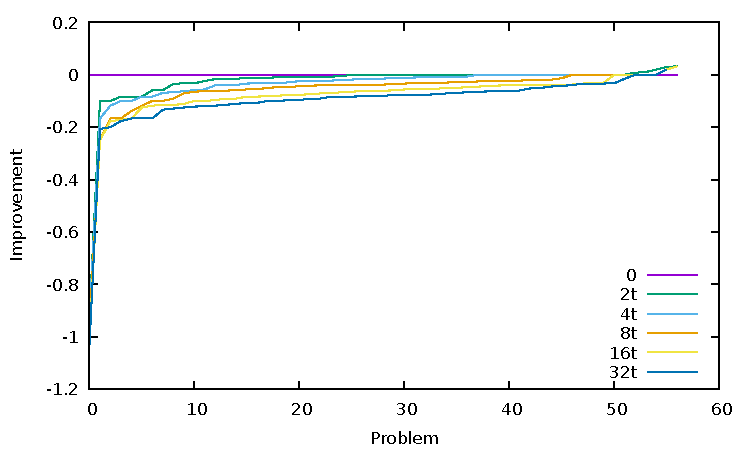
\includegraphics[scale = 1]{Experiments/E7/imp/impro.pdf}
      \caption{Advantage plot }
\end{figure} 
\begin{figure}[h!]
\centering
  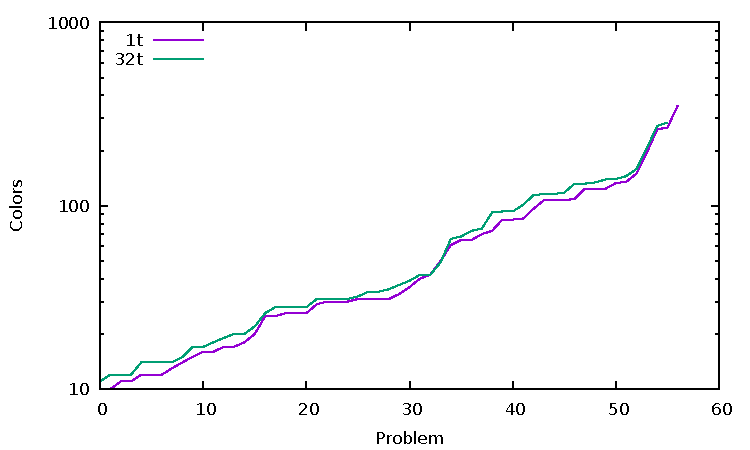
\includegraphics[scale = 1]{Experiments/E7/caclog.pdf}
      \caption{The performance of 32-thread tabu sharing GCP-solver is always worse than the performance of single-threaded GCP-solver}
\end{figure} 
\begin{table}[h!]
\caption{GCP-solver with tabu sharing. For c400.5, the performance with 32 thread is poor because of much memory swapping.}
\label{tab:tabu sharing}
\footnotesize
\begin{tabular}{|p{3cm} |p{1cm} p{1cm} p{1cm} p{1cm} p{1cm} p{1cm}|}
\hline
Graph&1t&2t&4t&8t&16t&32t\\ \hline
queen8\_8&\textbf{10}&11&11&11&11&12\\
le450\_5a&\textbf{11}&\textbf{11}&\textbf{11}&\textbf{11}&12&12\\
le450\_5b&\textbf{10}&11&11&11&11&11\\
queen9\_9&\textbf{11}&\textbf{11}&\textbf{11}&12&12&12\\ 
le450\_5c&\textbf{12}&13&13&15&15&14\\ \hline
le450\_5d&\textbf{12}&13&14&14&14&14\\ 
queen8\_12&\textbf{12}&13&13&14&13&14\\
queen10\_10&\textbf{13}&\textbf{13}&\textbf{13}&\textbf{13}&14&14\\ 
queen11\_11&\textbf{14}&\textbf{14}&\textbf{14}&15&15&15\\ 
queen12\_12&\textbf{15}&\textbf{15}&16&\textbf{15}&16&17\\ \hline
queen13\_13&\textbf{16}&\textbf{16}&17&17&17&18\\ 
dsjc500.1&\textbf{16}&\textbf{16}&\textbf{16}&17&18&17\\ 
queen14\_14&\textbf{17}&18&18&18&19&19\\ 
queen15\_15&\textbf{18}&\textbf{18}&19&19&20&20\\ 
le450\_15b&\textbf{17}&18&19&19&20&20\\ \hline
queen16\_16&\textbf{20}&\textbf{20}&\textbf{20}&\textbf{20}&21&22\\ 
le450\_15c&\textbf{26}&\textbf{26}&\textbf{26}&27&28&28\\ 
le450\_25a&\textbf{25}&\textbf{25}&26&26&27&28\\
le450\_25b&\textbf{25}&\textbf{25}&\textbf{25}&26&26&26\\ 
le450\_15d&\textbf{26}&\textbf{26}&27&27&29&28\\ \hline
dsjc1000.1&\textbf{26}&\textbf{26}&27&27&29&28\\
school1&33&\textbf{32}&33&35&35&37\\ 
school1\_nsh&\textbf{29}&30&31&33&34&35\\ 
zeroin.i.2&\textbf{30}&\textbf{30}&\textbf{30}&\textbf{30}&\textbf{30}&31\\
zeroin.i.3&\textbf{30}&\textbf{30}&\textbf{30}&\textbf{30}&31&31\\ \hline
fpsol2.i.3&31&\textbf{30}&\textbf{30}&\textbf{30}&\textbf{30}&31\\ 
fpsol2.i.2&\textbf{30}&\textbf{30}&31&31&\textbf{30}&31\\
le450\_25c&\textbf{31}&32&32&32&33&34\\ 
le450\_25d&\textbf{31}&32&32&33&34&34\\ 
miles750&\textbf{31}&\textbf{31}&32&\textbf{31}&32&32\\ \hline
dsjc250.5&\textbf{36}&\textbf{36}&\textbf{36}&38&38&39\\ 
flat300\_28\_0&\textbf{40}&\textbf{40}&\textbf{40}&41&42&42\\ 
miles1000&\textbf{42}&\textbf{42}&\textbf{42}&43&\textbf{42}&\textbf{42}\\
zeroin.i.1&50&\textbf{49}&\textbf{49}&\textbf{49}&\textbf{49}&\textbf{49}\\ 
dsjc500.5&\textbf{61}&62&\textbf{61}&64&66&68\\ \hline
fpsol2.i.1&\textbf{65}&\textbf{65}&\textbf{65}&\textbf{65}&\textbf{65}&66\\ 
r250.5&\textbf{70}&\textbf{70}&72&73&75&75\\ 
miles1500&\textbf{73}&\textbf{73}&\textbf{73}&\textbf{73}&\textbf{73}&\textbf{73}\\ 
brock400\_1&\textbf{84}&85&86&88&91&93\\ 
brock400\_2&\textbf{85}&86&86&88&89&92\\ \hline
brock400\_3&\textbf{84}&86&86&88&89&93\\ 
dsjr500.1c&96&\textbf{95}&96&100&102&101\\ 
flat1000\_60\_0&\textbf{107}&\textbf{107}&109&111&113&116\\
flat1000\_50\_0&\textbf{107}&\textbf{107}&108&109&111&116\\
flat1000\_76\_0&\textbf{107}&108&108&110&113&114\\ \hline
dsjc1000.5&\textbf{109}&110&111&112&114&118\\ 
r1000.1c&124&\textbf{123}&127&129&129&140\\ 
brock800\_1&\textbf{124}&125&126&127&129&132\\ 
brock800\_2&\textbf{124}&125&125&128&129&134\\ 
brock800\_4&\textbf{124}&125&125&127&130&132\\ \hline
latin\_square\_10&\textbf{135}&136&137&138&145&145\\ 
dsjr500.5&\textbf{133}&135&136&137&138&139\\
dsjc500.9&\textbf{150}&\textbf{150}&151&152&156&159\\ 
c2000.5&\textbf{195}&196&197&199&203&207\\ 
r1000.5&\textbf{261}&264&265&266&269&272\\ \hline
dsjc1000.9&\textbf{267}&271&270&275&278&284\\
c4000.5&\textbf{353}&356&356&362&372&545\\ \hline
\end{tabular}
\end{table}
\clearpage

\subsubsection{Experiment 8: GCP-solver with statistic Matrix sharing}
\label{sec:Experiment 8}
The statistic matrix is an important data structure in our implementation of GCP-solver to avoid long-term cycling in the local search. In experiment 4 \ref{sec:Experiment 4}, we found that with help of statistic matrix, the performance of our search in $55\%$ graphs is improved (see table \ref{tab:statistic matrix sharing}).
\begin{figure}[H]
  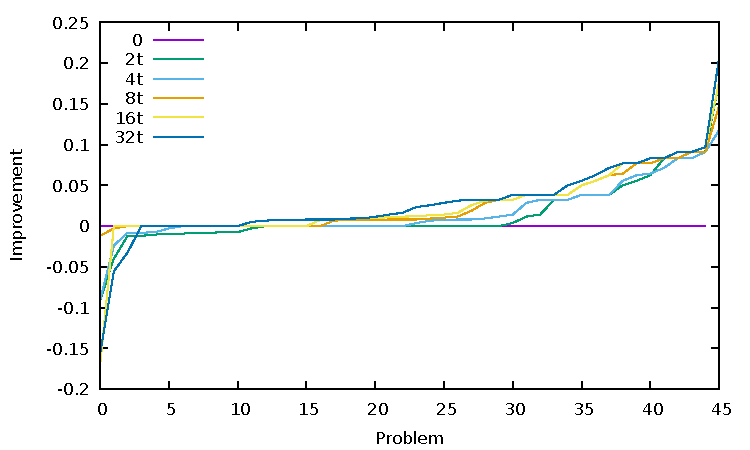
\includegraphics[scale = 1]{Experiments/E8/imp/impro.pdf}
  \caption{The improvement of GCP-solver through statistic matrix sharing is big. The improvement is however not stable.}
\end{figure}
\begin{table}[h!]
    \begin{tabular}{| l |l| l | l|l|l|p{1cm}|}
\hline
&1t&2t&4t&8t&16t&32t\\ \hline
best& 7&14&22&27&32&36\\ \hline
unique&1&0&0&2&4&6\\ \hline
    \end{tabular}
\captionof{table}{With more threads, the performance of our GCP-solver is improved through statistic matrix sharing. With 8 threads, more than half of the graphs have reached their minimum color size in local search.}
\end{table}

\begin{table}[h!]
\caption{46 of our 68 benchmark graphs have a different performance with GCP-solver using statistic matrix sharing. The GCP-solver with one thread is identical to the GCP-solver using a statistic matrix. Through experiment 4, we know the statistic solver itself brought an improvement to original GCP-solver.}
\label{tab:statistic matrix sharing}
\small
\begin{tabular}{|p{3cm}| p{1cm} p{1cm} p{1cm} p{1cm} p{1cm} p{1cm}|}
\hline
graph&1t&2t&4t&8t&16t&32t\\ \hline
queen8\_8&11&\textbf{10}&\textbf{10}&\textbf{10}&\textbf{10}&\textbf{10}\\
le450\_5b&11&\textbf{10}&11&\textbf{10}&\textbf{10}&\textbf{10}\\ 
queen9\_9&\textbf{11}&12&12&\textbf{11}&\textbf{11}&\textbf{11}\\
le450\_5c&12&\textbf{11}&\textbf{11}&\textbf{11}&\textbf{11}&\textbf{11}\\ 
le450\_5d&12&\textbf{11}&\textbf{11}&\textbf{11}&\textbf{11}&\textbf{11}\\ \hline
queen8\_12&13&13&13&\textbf{12}&\textbf{12}&\textbf{12}\\ 
queen10\_10&13&13&13&\textbf{12}&\textbf{12}&\textbf{12}\\ 
queen11\_11&14&14&\textbf{13}&14&14&\textbf{13}\\ 
dsjc500.1&16&\textbf{15}&\textbf{15}&\textbf{15}&\textbf{15}&\textbf{15}\\ 
queen14\_14&18&\textbf{17}&\textbf{17}&\textbf{17}&\textbf{17}&\textbf{17}\\ \hline
queen16\_16&20&\textbf{19}&20&\textbf{19}&\textbf{19}&\textbf{19}\\ 
le450\_15c&\textbf{25}&26&\textbf{25}&\textbf{25}&\textbf{25}&\textbf{25}\\
le450\_25a&26&\textbf{25}&\textbf{25}&\textbf{25}&\textbf{25}&\textbf{25}\\ 
le450\_25b&26&\textbf{25}&\textbf{25}&\textbf{25}&\textbf{25}&\textbf{25}\\
le450\_15d&26&\textbf{25}&26&\textbf{25}&\textbf{25}&\textbf{25}\\ \hline
dsjc1000.1&26&26&\textbf{25}&\textbf{25}&\textbf{25}&\textbf{25}\\
school1&34&28&30&29&28&\textbf{27}\\ 
school1\_nsh&31&30&29&29&\textbf{28}&\textbf{28}\\ 
zeroin.i.2&31&\textbf{30}&\textbf{30}&\textbf{30}&\textbf{30}&\textbf{30}\\ 
fpsol2.i.3&31&31&\textbf{30}&\textbf{30}&\textbf{30}&\textbf{30}\\ \hline
le450\_25c&31&31&\textbf{30}&31&31&\textbf{30}\\
miles750&\textbf{31}&\textbf{31}&\textbf{31}&\textbf{31}&\textbf{31}&32\\ 
dsjc250.5&35&35&\textbf{34}&\textbf{34}&35&\textbf{34}\\ 
flat300\_28\_0&39&39&39&39&\textbf{38}&\textbf{38}\\ 
inithx.i.1&\textbf{54}&\textbf{54}&\textbf{54}&\textbf{54}&\textbf{54}&57\\ \hline
dsjc500.5&61&61&61&61&61&\textbf{60}\\
r250.5&71&\textbf{70}&\textbf{70}&71&\textbf{70}&\textbf{70}\\
brock400\_1&84&85&86&85&\textbf{83}&84\\ 
brock400\_2&\textbf{84}&85&\textbf{84}&\textbf{84}&\textbf{84}&\textbf{84}\\ 
brock400\_3&85&84&84&84&84&\textbf{83}\\ \hline
dsjr500.1c&96&97&96&95&\textbf{93}&\textbf{93}\\
flat1000\_60\_0&\textbf{106}&107&\textbf{106}&\textbf{106}&\textbf{106}&\textbf{106}\\ 
flat1000\_50\_0&106&106&106&\textbf{104}&105&106\\ 
flat1000\_76\_0&107&107&\textbf{106}&107&\textbf{106}&\textbf{106}\\ 
dsjc1000.5&108&109&108&\textbf{107}&\textbf{107}&\textbf{107}\\ \hline
r1000.1c&123&123&122&122&\textbf{121}&122\\
brock800\_1&123&124&124&\textbf{122}&123&123\\ 
brock800\_2&124&125&125&\textbf{123}&124&\textbf{123}\\ 
brock800\_4&124&124&\textbf{123}&124&\textbf{123}&\textbf{123}\\
latin\_square\_10&133&134&\textbf{132}&\textbf{132}&133&133\\ \hline
dsjr500.5&134&135&135&134&134&\textbf{133}\\
dsjc500.9&149&149&148&148&\textbf{147}&148\\ 
c2000.5&194&194&194&194&194&\textbf{193}\\
r1000.5&263&263&263&261&261&\textbf{260}\\ 
dsjc1000.9&269&268&268&267&\textbf{266}&267\\
c4000.5&\textbf{352}&353&353&353&412&407\\ \hline
\end{tabular}
\end{table}


\subsubsection{Experiment 9: Comparison of our GCP-solver with other algorithms}
\label{sec:Experiment 9} 
In experiment 9, we compare our parallel GCP-solver with forced color reducing and statistic sharing with three other DSATUR-based algorithms: DSATUR algorithm, PASS algorithm, and TRICK algorithm (see table \ref{Dsatur}). The source code of DSATUR and PASS is supplied by Fabio Furini \cite{Dalgorithm}. The source code of the algorithm TRICK is provided by Michael Trick \cite{Trickalgorithm} (see details in \ref{comparison}). The benchmark graphs are tested with the same timeout as in our GCP solver algorithm (see \ref{benchmark}).
\begin{table}[!htbp]
\caption{comparison with DSATUR, PASS, and TRICK. The column $n$t is for $n$-thread GCP-solver with forced color reducing and statistic sharing. ``-'' means no result at the timeout. 50 of 68 (73\%) benchmark graphs get best results with our solver. 20 of 68 (29\%) benchmark graphs get unique best results with our solver.}
\label{Dsatur}
\scriptsize

\begin{tabular}{|p{2.5cm} |p{1cm} p{1cm} p{1cm} p{1cm} p{1cm} p{1cm} p{1.8cm} p{1cm} p{1cm}|}
\hline




Graph&1t&2t&4t&8t&16t&32t&DSATUR&PASS&TRICK\\ \hline
miles250&\textbf{8}&\textbf{8}&\textbf{8}&\textbf{8}&\textbf{8}&\textbf{8}&\textbf{8}&\textbf{8}&\textbf{8}\\ 
jean&\textbf{10}&\textbf{10}&\textbf{10}&\textbf{10}&\textbf{10}&\textbf{10}&\textbf{10}&\textbf{10}&\textbf{10}\\
queen8\_8&11&10&10&10&10&10&\textbf{9}&\textbf{9}&\textbf{9}\\
le450\_5a&10&10&10&10&10&10&\textbf{8}&9&9\\ 
le450\_5b&11&10&11&10&10&10&\textbf{9}&\textbf{9}&\textbf{9}\\ \hline
queen9\_9&11&12&11&11&11&11&\textbf{10}&\textbf{10}&\textbf{10}\\ 
le450\_5c&12&11&11&11&11&10&9&\textbf{5}&\textbf{5}\\ 
le450\_5d&12&11&11&11&11&10&10&9&\textbf{8}\\ 
queen8\_12&13&13&13&\textbf{12}&\textbf{12}&\textbf{12}&\textbf{12}&\textbf{12}&\textbf{12}\\ 
queen10\_10&13&13&13&\textbf{12}&\textbf{12}&\textbf{12}&\textbf{12}&\textbf{12}&\textbf{12}\\ \hline
queen11\_11&14&14&\textbf{13}&14&14&\textbf{13}&\textbf{13}&\textbf{13}&\textbf{13}\\
queen12\_12&15&15&15&15&15&\textbf{14}&15&15&15\\ 
queen13\_13&\textbf{16}&\textbf{16}&\textbf{16}&\textbf{16}&\textbf{16}&\textbf{16}&\textbf{16}&\textbf{16}&\textbf{16}\\ 
dsjc500.1&16&\textbf{15}&\textbf{15}&\textbf{15}&\textbf{15}&\textbf{15}&\textbf{15}&\textbf{15}&\textbf{15}\\ 
queen14\_14&18&\textbf{17}&\textbf{17}&\textbf{17}&\textbf{17}&\textbf{17}&18&\textbf{17}&\textbf{17}\\ \hline
queen15\_15&\textbf{18}&\textbf{18}&\textbf{18}&\textbf{18}&\textbf{18}&\textbf{18}&19&20&\textbf{18}\\ 
le450\_15b&18&18&18&18&18&18&\textbf{16}&\textbf{16}&\textbf{16}\\ 
miles500&\textbf{20}&\textbf{20}&\textbf{20}&\textbf{20}&\textbf{20}&\textbf{20}&\textbf{20}&\textbf{20}&\textbf{20}\\ 
queen16\_16&20&\textbf{19}&20&\textbf{19}&\textbf{19}&\textbf{19}&20&\textbf{19}&\textbf{19}\\ 
le450\_15c&25&26&25&25&25&25&\textbf{23}&\textbf{23}&\textbf{23}\\ \hline
le450\_25a&26&\textbf{25}&\textbf{25}&\textbf{25}&\textbf{25}&\textbf{25}&\textbf{25}&\textbf{25}&\textbf{25}\\
le450\_25b&\textbf{25}&\textbf{25}&\textbf{25}&\textbf{25}&\textbf{25}&\textbf{25}&\textbf{25}&\textbf{25}&\textbf{25}\\ 
le450\_15d&26&25&26&25&25&25&\textbf{23}&\textbf{23}&\textbf{23}\\ 
dsjc1000.1&26&26&\textbf{25}&\textbf{25}&\textbf{25}&\textbf{25}&26&26&-\\ 
school1&34&28&30&29&28&27&\textbf{14}&\textbf{14}&\textbf{14}\\ \hline
school1\_nsh&31&30&29&29&28&28&24&\textbf{14}&\textbf{14}\\
zeroin.i.2&31&\textbf{30}&\textbf{30}&\textbf{30}&\textbf{30}&\textbf{30}&\textbf{30}&\textbf{30}&\textbf{30}\\
zeroin.i.3&\textbf{30}&\textbf{30}&\textbf{30}&\textbf{30}&\textbf{30}&\textbf{30}&\textbf{30}&\textbf{30}&\textbf{30}\\ 
fpsol2.i.3&\textbf{30}&\textbf{30}&\textbf{30}&\textbf{30}&\textbf{30}&\textbf{30}&\textbf{30}&\textbf{30}&\textbf{30}\\ 
fpsol2.i.2&\textbf{30}&\textbf{30}&\textbf{30}&\textbf{30}&\textbf{30}&\textbf{30}&\textbf{30}&\textbf{30}&\textbf{30}\\  \hline
inithx.i.2&\textbf{31}&\textbf{31}&\textbf{31}&\textbf{31}&\textbf{31}&\textbf{31}&\textbf{31}&\textbf{31}&-\\ 
inithx.i.3&\textbf{31}&\textbf{31}&\textbf{31}&\textbf{31}&\textbf{31}&\textbf{31}&\textbf{31}&\textbf{31}&-\\ 
le450\_25c&31&31&30&31&31&30&\textbf{27}&28&28\\
le450\_25d&31&31&31&30&31&31&\textbf{27}&\textbf{27}&\textbf{27}\\
miles750&\textbf{31}&\textbf{31}&\textbf{31}&\textbf{31}&\textbf{31}&\textbf{31}&\textbf{31}&\textbf{31}&\textbf{31}\\\hline
mulsol.i.2&\textbf{31}&\textbf{31}&\textbf{31}&\textbf{31}&\textbf{31}&\textbf{31}&\textbf{31}&\textbf{31}&\textbf{31}\\ 
mulsol.i.3&\textbf{31}&\textbf{31}&\textbf{31}&\textbf{31}&\textbf{31}&\textbf{31}&\textbf{31}&\textbf{31}&\textbf{31}\\
mulsol.i.4&\textbf{31}&\textbf{31}&\textbf{31}&\textbf{31}&\textbf{31}&\textbf{31}&\textbf{31}&\textbf{31}&\textbf{31}\\ 
mulsol.i.5&\textbf{31}&\textbf{31}&\textbf{31}&\textbf{31}&\textbf{31}&\textbf{31}&\textbf{31}&\textbf{31}&\textbf{31}\\ 
dsjc250.5&35&35&\textbf{34}&\textbf{34}&35&\textbf{34}&-&-&35\\ \hline
flat300\_28\_0&39&39&39&39&\textbf{38}&\textbf{38}&41&40&39\\ 
miles1000&\textbf{42}&\textbf{42}&\textbf{42}&\textbf{42}&\textbf{42}&\textbf{42}&\textbf{42}&\textbf{42}&\textbf{42}\\
mulsol.i.1&\textbf{49}&\textbf{49}&\textbf{49}&\textbf{49}&\textbf{49}&\textbf{49}&\textbf{49}&\textbf{49}&\textbf{49}\\ 
zeroin.i.1&\textbf{49}&\textbf{49}&\textbf{49}&\textbf{49}&\textbf{49}&\textbf{49}&\textbf{49}&\textbf{49}&\textbf{49}\\
inithx.i.1&\textbf{54}&\textbf{54}&\textbf{54}&\textbf{54}&\textbf{54}&\textbf{54}&\textbf{54}&\textbf{54}&-\\ \hline
dsjc500.5&61&61&61&61&61&\textbf{60}&63&64&63\\
fpsol2.i.1&\textbf{65}&\textbf{65}&\textbf{65}&\textbf{65}&\textbf{65}&\textbf{65}&\textbf{65}&\textbf{65}&\textbf{65}\\ 
r250.5&71&70&70&71&70&70&\textbf{66}&67&-\\ 
miles1500&\textbf{73}&\textbf{73}&\textbf{73}&\textbf{73}&\textbf{73}&\textbf{73}&\textbf{73}&\textbf{73}&\textbf{73}\\
brock400\_1&84&85&85&84&\textbf{83}&\textbf{83}&90&90&89\\ \hline
brock400\_2&\textbf{84}&85&\textbf{84}&\textbf{84}&\textbf{84}&\textbf{84}&90&91&91\\ 
brock400\_3&85&84&84&84&84&\textbf{83}&90&89&90\\ 
dsjr500.1c&95&94&94&95&93&93&-&-&\textbf{88}\\ 
flat1000\_60\_0&\textbf{106}&107&\textbf{106}&\textbf{106}&\textbf{106}&\textbf{106}&111&113&-\\ 
flat1000\_50\_0&106&106&106&\textbf{104}&105&106&114&112&-\\ \hline
flat1000\_76\_0&107&107&\textbf{106}&107&\textbf{106}&\textbf{106}&114&111&-\\ 
dsjc1000.5&108&109&108&\textbf{107}&\textbf{107}&\textbf{107}&116&114&-\\ 
r1000.1c&123&123&122&122&120&\textbf{119}&-&-&\\
brock800\_1&123&124&124&\textbf{122}&123&123&133&132&-\\ brock800\_2&124&124&124&123&124&\textbf{123}&132&131&-\\ \hline
brock800\_4&124&124&\textbf{123}&124&\textbf{123}&\textbf{123}&&131&-\\ 
latin\_square\_10&133&134&132&132&132&132&\textbf{130}&140&-\\ 
dsjr500.5&134&135&135&134&134&133&131&134&\textbf{130}\\ 
dsjc500.9&149&149&148&148&\textbf{147}&148&-&-&160\\ 
c2000.5&194&194&194&194&194&\textbf{193}&208&204&-\\ \hline
r1000.5&263&263&263&261&261&260&250&\textbf{245}&-\\ 
dsjc1000.9&269&268&268&267&\textbf{266}&267&297&300&-\\ 
c4000.5&\textbf{352}&353&353&353&386&\textbf{352}&377&376&-\\ \hline

\end{tabular}
\end{table}
\clearpage
\section{Conclusion}
The scheme of finding a legal $k$-coloring of a graph and then reducing the size in search iteratively to find the minimum color size, is universally applicable to GCP algorithms. Our paper presents a parallel cooperative algorithm to solve GCP with this scheme. The local search used in our algorithm is a tabu search called Tabucol.\\

In section \ref{sec:Solving GCP by Tabucol}, we discuss the three steps of this scheme: solution initialization, k-GCP solution and color reduction. To each step, we  give a suggestion in implementation to improve the performance of our algorithm. In \ref{subsec:Improvement through randomly generated solution}, we compare the GCP-solver with a randomly generated initial solution and the version with an $n$-coloring which takes node indices as the initial color indices. The interesting fact is that the node-index initialization is advantageous in the result and also in execution time because of its simplicity. For the $k$-GCP solution, we discuss the way of choosing the next move if several critical moves exist with the maximal improvement. For the color reduction, we always reduce the least used color in the current solution. Apart from discussing the process of the GCP-solver, we introduce the data structures in our implementation. We add a matrix data structure called statistic matrix in our implementation, which supports the recognition of long-term cycling in tabu search and therefore improves the performance of our GCP-solver.\\

Most graphs get better results with the suggestions in our single-threaded GCP-solver. However, some graphs get better results with the original GCP-solver. With this observation, we make our GCP-solver parallel with different parameter combinations in agents. In this way, the agents run the search with some different settings and then take advantage of the reasonable combinations of the suggestions.\\

In section \ref{sec:Our parallel Algorithm}, we discussed the exchange of information among the agents in a parallel search. The first approach is minimum size exchange, in which the agents exchange the found color size. The approach, whose initial purpose is to save search time, was found experimentally to bring also an improvement on results.\\
Then we shared the information of the local search cycling among the agents. We tested the exchange of statistic matrix in the search process since tabu list sharing turned out to be a failed attempt. We found the statistic matrix sharing brings further improvement.\\

With experiments, the hypothesis was evaluated that certain information exchange among agents can improve the performance of the parallel search. 
\subsection{Further work}
While this thesis has demonstrated the potential of cooperation of parallel searches for the GCP, many opportunities of other investigation directions remain. This section presents some of these directions.\\

\emph{\textbf{Using different  search strategies}}\\
In our algorithm, we use the k-GCP algorithm Tabucol as the subroutine. In further research, the agents can use a different search strategy. It is to investigate, whether our introduced cooperation is only beneficial for our tabu local search or generally applicable.\\

\emph{\textbf{Using different cooperation strategies}}\\
In this thesis, the cooperation is limited to information exchange. Some other directions like generic population-based metaheuristic are definitely worth further research.\\

\emph{\textbf{Using different algorithms in agents}}\\
In our GCP-solver, all the agents run the same GCP algorithms. An interesting topic is the cooperation of agents, which run different GCP algorithms.
\clearpage
\section{Bibliography}
\bibliographystyle{ieeetr}
\bibliography{references}
\end{document}
